\documentclass[12pt,a4paper]{article}
\usepackage[utf8]{inputenc}
\usepackage[T1]{fontenc}
\usepackage[ngerman]{babel}
\usepackage{geometry}
\geometry{a4paper, margin=2.5cm}
\usepackage{setspace}
\usepackage{amsmath, amssymb, amsthm}
\usepackage{mathtools}
\usepackage{pgfplots}
\pgfplotsset{compat=1.18}
\usepackage{tikz}
\usetikzlibrary{shapes.geometric, arrows.meta, positioning, fit, backgrounds}
\usepackage{booktabs}
\usepackage{array}
\usepackage{multirow}
\usepackage{microtype}
\usepackage{graphicx}
\usepackage{caption}
\usepackage{rotating}
\usepackage{subcaption}
\usepackage{float}
\usepackage{hyperref}
\hypersetup{
	colorlinks=true,
	linkcolor=blue!60!black,
	citecolor=green!50!black,
	urlcolor=blue,
	pdftitle={KI-gesteuertes Power Management fuer Lithium-Ionen-Akkumulatoren},
	pdfauthor={Stephan Epp},
}
\usepackage{algorithm2e}
\usepackage{listings}
\usepackage{xcolor}
\usepackage{enumitem}
\usepackage{fancyhdr}
\usepackage{titlesec}
\usepackage{abstract}
\usepackage{tocloft}
\usepackage{enumitem}
\setlist[itemize,1]{label=--}

% --- Theoreme ---
\newtheorem{theorem}{Theorem}[section]
\newtheorem{lemma}[theorem]{Lemma}
\newtheorem{corollary}[theorem]{Korollar}
\newtheorem{proposition}[theorem]{Proposition}
\newtheorem{definition}{Definition}[section]
\newtheorem{remark}{Bemerkung}[section]

% --- Farben ---
\definecolor{mainblue}{RGB}{0,70,140}
\definecolor{accentred}{RGB}{180,30,30}
\definecolor{codegreen}{rgb}{0,0.6,0}
\definecolor{codegray}{rgb}{0.5,0.5,0.5}
\definecolor{backcolour}{rgb}{0.97,0.97,0.97}

\lstdefinestyle{pythonstyle}{
	backgroundcolor=\color{backcolour},
	commentstyle=\color{codegreen},
	keywordstyle=\color{mainblue},
	numberstyle=\tiny\color{codegray},
	stringstyle=\color{accentred},
	basicstyle=\ttfamily\footnotesize,
	breaklines=true,
	numbers=left,
	frame=single,
	language=Python
}

% ============================================================
\begin{document}
	% ============================================================
	
	% --- Titelseite ---
	\begin{titlepage}
		\centering
		\vspace*{1.5cm}
		\vspace{0.5cm}
		{\Huge\bfseries
			KI-Power-Management-Modul für Lithium-Ionen-Akkumulatoren
			\par}
		{\large\itshape
			Formaler Nachweis der Ãœberlegenheit eines lernenden,\\
			verhaltensadaptiven Power-Management-Systems
			\par}
		\vspace{1.5cm}
		{\large
			\begin{tabular}{rl}
				\textbf{Autor:}      & Stephan Epp \\[4pt]
				\textbf{Datum:}      & 7. März 2026 \\[4pt]
			\end{tabular}
		}
	\end{titlepage}
	
	% --- Abstract ---
	\begin{abstract}
		\noindent
		Lithium-Ionen-Akkumulatoren (LIB) sind die dominierende Energiespeichertechnologie
		in mobilen Geräten, Elektrofahrzeugen und stationären Speichersystemen.
		Ihre Lebensdauer wird maßgeblich durch zwei physikalische Hauptmechanismen
		begrenzt: (1) temperaturinduziertes Kapazitätsdriften und (2) elektrochemische
		Degradation durch unkontrollierte Zellspannungen. Konventionelle Power-Management-Systeme
		(PMS) adressieren diese Mechanismen reaktiv anhand statischer Schwellwerte.
		
		Diese Arbeit präsentiert ein formal nachgewiesenes, KI-getriebenes Power-Manage\-ment-Modul
		(AI-PMM), das Nutzungsverhalten und Umgebungsparameter kontinuierlich erlernt
		und prädiktiv in Regelstrategien umsetzt. Mithilfe eines Reinforcement-Learning-Agenten
		sowie adaptiver Regler werden Temperatur und Zellspannung dynamisch optimiert.
		
		Es wird mathematisch hergeleitet, dass das AI-PMM gegenüber einem statischen
		Referenz-PMS die Gesamtlebensdauer um den Faktor $\Phi \geq 1{,}47$ steigert.
		Formale Stabilitätsanalysen (Lyapunov) und Degradationsmodelle (Arrhenius,
		SEI-Wachstum) belegen die theoretische Fundierung. Simulationsergebnisse mit
		synthetischen Lastprofilen bestätigen die analytischen Resultate.
	\end{abstract}
	
	\vspace{1cm}
	\noindent\textbf{Schlüsselwörter:} Lithium-Ionen-Akkumulator, Power Management,
	Künstliche Intelligenz, Reinforcement Learning, Lebensdauermaximierung,
	Temperaturregelung, Spannungsregelung, SEI-Schicht, Arrhenius-Modell, Lyapunov-Stabilität.
	
	\newpage
	\tableofcontents
	\newpage
	
	% ============================================================
	\section{Einleitung}
	% ============================================================
	
	\subsection{Motivation und Problemstellung}
	
	Lithium-Ionen-Akkumulatoren haben sich seit ihrer kommerziellen Einführung Anfang
	der 1990er Jahre als Schlüsseltechnologie für mobile Energiespeicherung etabliert.
	Mit einer gravimetrischen Energiedichte von typischerweise
	$150\text{--}300\,\mathrm{Wh\,kg^{-1}}$ und einer volumetrischen Energiedichte
	von $250\text{--}700\,\mathrm{Wh\,L^{-1}}$ übertreffen sie konkurrierende
	Technologien wie Nickel-Metallhydrid- oder Blei-Säure-Akkumulatoren deutlich
	\cite{Tarascon2001}.
	
	Gleichwohl unterliegen LIB einem unvermeidlichen Alterungsprozess, der durch
	zwei dominierende Mechanismen gesteuert wird:
	
	\begin{enumerate}[leftmargin=*, label=(\arabic*)]
		\item \textbf{Thermisch induzierte Alterung:} Erhöhte Temperaturen beschleunigen
		die Bildung der Solid-Electrolyte-Interphase (SEI) an der Anodenoberfläche,
		fördern Lithium-Plating, und führen zu mechanischen Spannungen durch
		anisotropes Gitterausdehnen. Das resultierende Kapazitätsdriften ist
		in erster Näherung arrheniusförmig \cite{Wang2011}.
		
		\item \textbf{Elektrochemisch induzierte Alterung:} Ãœber- und Unterspannungen
		jenseits des zulässigen Betriebsbereichs initiieren irreversible Phasenumwandlungen
		in Kathoden- und Anodenmaterialien, Elektrolytoxidation sowie Lithium-Dendritenbildung
		\cite{Aurbach2002}.
	\end{enumerate}
	
	Konventionelle Power-Management-Systeme begegnen diesen Mechanismen durch statische
	Grenzwerte (z.\,B.\ $2{,}5\,\mathrm{V} \leq V_\mathrm{cell} \leq 4{,}2\,\mathrm{V}$,
	$-20\,^\circ\mathrm{C} \leq T \leq 45\,^\circ\mathrm{C}$). Diese Grenzwerte sind
	jedoch konservativ und ignorieren den kontextabhängigen Betriebszustand sowie
	das individuelle Nutzerverhalten. Ein lernendes System kann diese Grenzen
	adaptiv und prädiktiv nutzen, um die Gesamtlebensdauer zu maximieren.
	
	\subsection{Zielsetzung und Beitrag}
	
	Diese Arbeit leistet folgende wissenschaftliche Beiträge:
	
	\begin{itemize}[leftmargin=*]
		\item Formale Modellierung der temperatur- und spannungsbedingten Degradation
		von LIB durch etablierte elektrochemische und thermodynamische Modelle.
		\item Entwurf eines KI-gesteuerten Power-Management-Moduls (AI-PMM) basierend
		auf Deep Reinforcement Learning (DRL) mit expliziter Modellierung von Nutzungsverhalten
		und Umgebungsparametern.
		\item Mathematischer Nachweis der Lebensdauerüberlegenheit des AI-PMM gegenüber
		einem statischen Referenzsystem mittels Degradationsintegral und Lyapunov-Analyse.
		\item Simulation und Validierung an realistischen Lastprofilen.
	\end{itemize}
	
	% ============================================================
	\section{Grundlagen der LIB-Degradation}
	\label{sec:grundlagen}
	% ============================================================
	
	\subsection{Elektrochemische Grundprinzipien}
	
	Eine Lithium-Ionen-Zelle besteht aus Anode (üblicherweise Graphit $\mathrm{LiC_6}$),
	Kathode (z.\,B.\ $\mathrm{LiCoO_2}$, $\mathrm{LiFePO_4}$, NMC), Elektrolyt
	und Separator. Die Gleichgewichtsspannung einer NMC/Graphit-Zelle berechnet sich
	zu:
	
	\begin{equation}
		E_\mathrm{cell} = E^\circ_\mathrm{Kathode} - E^\circ_\mathrm{Anode}
		+ \frac{RT}{nF}\ln\frac{a_\mathrm{Ox}}{a_\mathrm{Red}}
		\label{eq:nernst}
	\end{equation}
	
	wobei $R = 8{,}314\,\mathrm{J\,mol^{-1}\,K^{-1}}$ die universelle Gaskonstante,
	$T$ die absolute Temperatur, $n$ die Anzahl übertragener Elektronen, $F =
	96485\,\mathrm{C\,mol^{-1}}$ die Faraday-Konstante und $a_i$ die Aktivitäten
	der Reaktanden sind.
	
	\subsection{Thermische Degradationsmechanismen}
	\label{subsec:therm_deg}
	
	\subsubsection{SEI-Wachstum}
	
	Die Solid-Electrolyte-Interphase (SEI) bildet sich irreversibel an der
	Grenzfläche Anode/Elektrolyt durch Elektrolytreduktion. Die SEI-Dicke
	$\delta_\mathrm{SEI}(t)$ wächst nach einem wurzelförmigen Gesetz:
	
	\begin{equation}
		\frac{d\delta_\mathrm{SEI}}{dt} = \frac{k_\mathrm{SEI}}{2\delta_\mathrm{SEI}}
		\exp\!\left(-\frac{E_{a,\mathrm{SEI}}}{RT}\right)
		\label{eq:sei_growth}
	\end{equation}
	
	Daraus folgt durch Integration:
	
	\begin{equation}
		\delta_\mathrm{SEI}(t) = \sqrt{2 k_\mathrm{SEI} t \exp\!\left(-\frac{E_{a,\mathrm{SEI}}}{RT}\right)}
		\propto \sqrt{t}
		\label{eq:sei_sqrt}
	\end{equation}
	
	Der kapazitative Verlust $\Delta Q_\mathrm{SEI}$ ist proportional zur SEI-Dicke
	(da Lithium irreversibel in der SEI gebunden wird):
	
	\begin{equation}
		\Delta Q_\mathrm{SEI}(t) = \alpha_\mathrm{SEI} \cdot \delta_\mathrm{SEI}(t)
		\label{eq:cap_loss_sei}
	\end{equation}
	
	\subsubsection{Arrhenius-Beschleunigung}
	
	Die Temperaturabhängigkeit aller relevanten Degradationsraten folgt dem
	Arrhenius-Gesetz:
	
	\begin{equation}
		k(T) = A \exp\!\left(-\frac{E_a}{RT}\right)
		\label{eq:arrhenius}
	\end{equation}
	
	Die relative Beschleunigung der Degradationsrate bei Temperaturerhöhung von
	$T_0$ auf $T$ beträgt:
	
	\begin{equation}
		\frac{k(T)}{k(T_0)} = \exp\!\left[\frac{E_a}{R}\left(\frac{1}{T_0}-\frac{1}{T}\right)\right]
		\label{eq:arrhenius_ratio}
	\end{equation}
	
	Für $E_a = 50\,\mathrm{kJ\,mol^{-1}}$ (typisch für SEI-Wachstum \cite{Wang2011}),
	$T_0 = 298\,\mathrm{K}$ und $T = 318\,\mathrm{K}$ ($+20\,\mathrm{K}$) ergibt sich:
	
	\begin{equation}
		\frac{k(318)}{k(298)} = \exp\!\left[\frac{50000}{8{,}314}\cdot
		\left(\frac{1}{298}-\frac{1}{318}\right)\right] \approx 2{,}77
	\end{equation}
	
	\textbf{Schlussfolgerung:} Eine Temperaturerhöhung um $20\,\mathrm{K}$ nahezu
	verdreifacht die SEI-Wachstumsrate und damit die Kapazitätsverlustrate.
	
	\subsubsection{Kapazitätsdriften -- formale Definition}
	
	\begin{definition}[Kapazitätsdriften]
		Das Kapazitätsdriften $\mathcal{D}(t)$ einer LIB-Zelle ist definiert als
		die normierte zeitliche Abnahme der nutzbaren Kapazität:
		\begin{equation}
			\mathcal{D}(t) \coloneqq 1 - \frac{Q(t)}{Q_0}
		\end{equation}
		wobei $Q_0$ die Nominalkapazität und $Q(t)$ die aktuelle Kapazität bezeichnet.
		\textit{End-of-Life} (EoL) wird üblicherweise bei $\mathcal{D}(t_\mathrm{EoL}) = 0{,}20$
		(80\,\% der Nominalkapazität) definiert.
	\end{definition}
	
	\subsection{Spannungsbedingte Degradationsmechanismen}
	\label{subsec:volt_deg}
	
	\subsubsection{Ãœberspannungsdegradation}
	
	Bei Ãœberschreiten der oberen Grenzspannung $V_\mathrm{max}$ (typisch
	$4{,}2\,\mathrm{V}$ für NMC) treten auf:
	
	\begin{itemize}
		\item Elektrolytoxidation: $\mathrm{EC} \rightarrow \text{Oxidationsprodukte}$ bei
		$V > 4{,}3\,\mathrm{V}$
		\item Strukturelle Phasenumwandlungen der Kathode (z.\,B.\ layered $\to$ spinel $\to$ rock salt)
		\item Sauerstofffreisetzung bei extremer Ãœberladung (Sicherheitsrisiko)
	\end{itemize}
	
	Die Degradationsrate durch Ãœberspannung wird modelliert als:
	
	\begin{equation}
		r_\mathrm{OV}(V) = \begin{cases}
			0 & V \leq V_\mathrm{max} \\
			k_\mathrm{OV} \exp\!\left(\beta_\mathrm{OV}(V - V_\mathrm{max})\right) - k_\mathrm{OV}
			& V > V_\mathrm{max}
		\end{cases}
		\label{eq:overvoltage_rate}
	\end{equation}
	
	\subsubsection{Unterspannungsdegradation und Lithium-Plating}
	
	Bei tiefer Entladung ($V < V_\mathrm{min}$, typisch $2{,}5\,\mathrm{V}$) und
	bei Schnellladung bei niedrigen Temperaturen besteht die Gefahr des Lithium-Platings:
	metallisches Lithium scheidet sich statt in die Graphitstruktur intercaliert zu werden
	an der Anodenoberfläche ab. Dies führt zu:
	
	\begin{itemize}
		\item Irreversiblem Lithiumverlust (``dead Lithium'')
		\item Dendritenwachstum (Kurzschlusskurzschlussgefahr)
		\item Beschleunigter SEI-Reformation
	\end{itemize}
	
	Der kritische Stromdichte-Schwellwert für Lithium-Plating ist:
	
	\begin{equation}
		j_\mathrm{plating}(T) = j_0 \exp\!\left(\frac{-E_{a,\mathrm{plating}}}{RT}\right) \cdot
		\frac{F}{RT}\left(V_\mathrm{Li^+/Li} - \phi_\mathrm{anode}\right)
		\label{eq:li_plating}
	\end{equation}
	
	\subsubsection{Spannungsfenster-Optimierung}
	
	Das effektive Nutzungsfenster $[V_\mathrm{min}^*, V_\mathrm{max}^*]$ minimiert
	die Gesamtdegradationsrate. Das Optimierungsproblem lautet:
	
	\begin{equation}
		[V_\mathrm{min}^*, V_\mathrm{max}^*] = \arg\min_{V_l, V_u}
		\int_0^{t_\mathrm{op}} \left[r_\mathrm{OV}(V(t)) + r_\mathrm{UV}(V(t))\right] dt
		\label{eq:voltage_window_opt}
	\end{equation}
	
	unter der Nebenbedingung, dass die nutzbare Energiemenge für den Betrieb
	ausreicht:
	
	\begin{equation}
		\int_{V_l}^{V_u} C(V)\, dV \geq E_\mathrm{req}
	\end{equation}
	
	% ============================================================
	\section{Formales Degradationsmodell}
	\label{sec:degradationsmodell}
	% ============================================================
	
	\subsection{Zustandsraumdarstellung}
	
	Der Zustand einer LIB-Zelle wird durch den Zustandsvektor
	
	\begin{equation}
		\mathbf{x}(t) = \bigl[Q(t),\; T(t),\; V(t),\; \delta_\mathrm{SEI}(t),\; R_\mathrm{int}(t)\bigr]^\top
		\label{eq:state_vector}
	\end{equation}
	
	beschrieben, wobei $R_\mathrm{int}$ den Innenwiderstand bezeichnet. Die
	Systemdynamik ergibt sich zu:
	
	\begin{equation}
		\dot{\mathbf{x}}(t) = \mathbf{f}\bigl(\mathbf{x}(t), \mathbf{u}(t), \boldsymbol{\theta}(t)\bigr)
		\label{eq:state_space}
	\end{equation}
	
	mit dem Steuervektor $\mathbf{u}(t) = [I(t),\; T_\mathrm{set}(t)]^\top$
	(Ladestrom und Solltemperatur) und Umgebungsparametern $\boldsymbol{\theta}(t)$.
	
	\subsection{Gesamtdegradationsrate}
	
	Die Gesamtdegradationsrate setzt sich additiv aus kalendarischen und zyklischen
	Beiträgen zusammen:
	
	\begin{equation}
		\dot{\mathcal{D}}(t) = \underbrace{\gamma_T \cdot k_\mathrm{SEI}(T(t))}_{\text{thermisch}}
		+ \underbrace{\gamma_V \cdot r_\mathrm{volt}(V(t))}_{\text{spannungsbedingt}}
		+ \underbrace{\gamma_C \cdot r_\mathrm{cycle}(I(t), T(t))}_{\text{zyklisch}}
		\label{eq:total_degradation}
	\end{equation}
	
	mit Gewichtungskoeffizienten $\gamma_T, \gamma_V, \gamma_C > 0$, die materialspezifisch
	sind.
	
	\subsection{Kumuliertes Degradationsintegral}
	
	\begin{definition}[Kumuliertes Degradationsintegral]
		Die Gesamtalterung bis zum Zeitpunkt $t$ ist:
		\begin{equation}
			\Psi(t) = \int_0^t \dot{\mathcal{D}}(\tau)\, d\tau
			\label{eq:deg_integral}
		\end{equation}
		EoL tritt ein, wenn $\Psi(t_\mathrm{EoL}) = \mathcal{D}_\mathrm{EoL} = 0{,}20$.
	\end{definition}
	
	Die Lebensdauer $L$ ist damit:
	
	\begin{equation}
		L = t_\mathrm{EoL} = \Psi^{-1}(\mathcal{D}_\mathrm{EoL})
		= \left(\int_0^{L} \dot{\mathcal{D}}(\tau)\, d\tau\right)^{-1} \mathcal{D}_\mathrm{EoL}
		\label{eq:lifetime}
	\end{equation}
	
	\subsection{Thermisches Netzwerkmodell}
	
	Die Zelltemperatur wird durch ein vereinfachtes Wärmenetzwerk modelliert:
	
	\begin{equation}
		m_\mathrm{cell} c_p \dot{T}(t) = \dot{Q}_\mathrm{gen}(t) - \frac{T(t) - T_\mathrm{amb}(t)}{R_\mathrm{th}}
		\label{eq:thermal_model}
	\end{equation}
	
	mit Wärmeerzeugungsrate:
	
	\begin{equation}
		\dot{Q}_\mathrm{gen}(t) = I(t)^2 R_\mathrm{int}(t) +
		I(t)\cdot T(t)\frac{\partial E_\mathrm{cell}}{\partial T}
		\label{eq:heat_gen}
	\end{equation}
	
	Der erste Term entspricht der Joule'schen Verlustleistung, der zweite Term
	der reversiblen Wärme (entropischer Beitrag).
	
	% ============================================================
	\section{KI-gesteuertes Power-Management-Modul (AI-PMM)}
	\label{sec:ai_pmm}
	% ============================================================
	
	\subsection{Systemarchitektur}
	
	Das AI-PMM integriert drei Hauptkomponenten:
	
	\begin{enumerate}[leftmargin=*, label=(\Roman*)]
		\item \textbf{Sensorschicht:} Erfassung von $T, V, I, T_\mathrm{amb}$
		mit Abtastrate $f_s = 10\,\mathrm{Hz}$.
		\item \textbf{Kognitiver Kern:} Deep-RL-Agent mit Nutzerverhaltensmodell.
		\item \textbf{Aktionsschicht:} Temperaturregler (PID + Feedforward) und
		Spannungsregler (Model Predictive Control).
	\end{enumerate}
	
	\begin{sidewaysfigure}
		\centering
		\begin{tikzpicture}[
			node distance=1.2cm and 1.8cm,
			every node/.style={font=\small},
			box/.style={rectangle, draw, rounded corners=3pt, minimum height=1.0cm,
				minimum width=3.0cm, align=center, fill=blue!8},
			ai/.style={rectangle, draw, rounded corners=3pt, minimum height=1.8cm,
				minimum width=4.5cm, align=center, fill=orange!15, thick},
			sensor/.style={rectangle, draw, rounded corners=3pt, minimum height=0.9cm,
				minimum width=2.5cm, align=center, fill=green!12},
			act/.style={rectangle, draw, rounded corners=3pt, minimum height=0.9cm,
				minimum width=2.5cm, align=center, fill=red!12},
			arr/.style={->, >=Latex, thick}
			]
			
			\node[sensor] (sens) {Sensorschicht\\$T, V, I, T_\mathrm{amb}$};
			\node[box, right=of sens] (feat) {Feature\\Extraktion};
			\node[ai, right=of feat] (rl) {Deep-RL-Agent\\(DQN/PPO)\\+ Verhaltensmodell};
			\node[box, right=of rl] (ctrl) {Temperatur-\\regler (PID)\\Spannungs-\\regler (MPC)};
			\node[act, right=of ctrl] (bat) {LIB-Zelle\\(Aktuatoren)};
			
			\node[box, below=1.5cm of rl] (mem) {Erfahrungs-\\speicher\\(Replay Buffer)};
			
			\draw[arr] (sens) -- (feat);
			\draw[arr] (feat) -- (rl);
			\draw[arr] (rl) -- (ctrl);
			\draw[arr] (ctrl) -- (bat);
			\draw[arr] (bat.south) -- ++(0,-0.9) -| (sens.south);
			\draw[arr] (rl) -- (mem);
			\draw[arr] (mem.east) -- ++(0.5,0) |- (rl.south);
			
		\end{tikzpicture}
		\caption{Systemarchitektur des AI-PMM. Der Regelkreis umfasst Sensorik,
			kognitiven Kern und Aktionsschicht mit Rückkopplung über Erfahrungsspeicher.}
		\label{fig:architecture}
	\end{sidewaysfigure}
	
	\subsection{Markov-Entscheidungsprozess (MDP)}
	
	Das Steuerungsproblem wird als MDP $\mathcal{M} = (\mathcal{S}, \mathcal{A}, \mathcal{P}, \mathcal{R}, \gamma_\mathrm{RL})$
	formalisiert:
	
	\begin{itemize}[leftmargin=*]
		\item \textbf{Zustandsraum} $\mathcal{S}$: $\mathbf{s}(t) = [\text{SoC}(t), T(t), V(t), I(t),
		T_\mathrm{amb}(t), \hat{\mathbf{b}}(t), \hat{\boldsymbol{\psi}}(t)]$,
		wobei $\hat{\mathbf{b}}(t)$ das gelernte Nutzerverhaltensvektor und
		$\hat{\boldsymbol{\psi}}(t)$ der prognostizierte Degradationszustand.
		
		\item \textbf{Aktionsraum} $\mathcal{A}$: Diskretisiert in
		$N_T = 20$ Temperatursollwerte $\times$ $N_V = 20$ Spannungssollwerte
		$\Rightarrow |\mathcal{A}| = 400$.
		
		\item \textbf{Belohnungsfunktion} $\mathcal{R}$: Gewichtet Degradation
		gegen Nutzbarkeit:
		\begin{equation}
			r(t) = -\lambda_1 \dot{\mathcal{D}}(t) + \lambda_2 \eta_\mathrm{use}(t)
			- \lambda_3 \|\mathbf{a}(t) - \mathbf{a}(t-1)\|^2
			\label{eq:reward}
		\end{equation}
		mit Hyperparametern $\lambda_1, \lambda_2, \lambda_3 > 0$.
		
		\item \textbf{Diskontierungsfaktor} $\gamma_\mathrm{RL} = 0{,}99$ (langfristige Optimierung).
	\end{itemize}
	
	\subsection{Nutzerverhaltensmodell}
	
	Das AI-PMM erlernt ein probabilistisches Modell des Nutzerverhaltens:
	
	\begin{equation}
		p\bigl(\mathbf{u}_{t+k} \mid \mathbf{s}_{1:t}, \mathbf{c}_{1:t}\bigr)
		\approx \mathcal{N}\bigl(\boldsymbol{\mu}_\theta(t), \boldsymbol{\Sigma}_\theta(t)\bigr)
		\label{eq:user_model}
	\end{equation}
	
	wobei $\mathbf{c}(t)$ Kontextinformationen (Tageszeit, Wochentag, Standort,
	Aktivitätsmuster) enthält. Dieses Modell wird durch ein rekurrentes neuronales
	Netz (LSTM) mit $H = 128$ versteckten Einheiten approximiert:
	
	\begin{equation}
		\hat{\mathbf{u}}_{t+1:t+K} = \mathrm{LSTM}_\theta\bigl(\mathbf{s}_{t-\tau:t},
		\mathbf{c}_{t-\tau:t}\bigr)
		\label{eq:lstm_prediction}
	\end{equation}
	
	Die prädiktive Last $K$ Schritte voraus ermöglicht präemptives Kühlmanagement.
	
	\subsection{Adaptiver Temperaturregler}
	
	Der Temperaturregler kombiniert einen PID-Regler mit einem lernenden Feedforward-Anteil:
	
	\begin{align}
		u_T(t) &= K_p e_T(t) + K_i \int_0^t e_T(\tau)\,d\tau + K_d \dot{e}_T(t)
		+ u_\mathrm{FF}(\hat{\mathbf{u}}_{t+1:t+K}, \hat{T}_\mathrm{amb})
		\label{eq:pid_controller}
	\end{align}
	
	wobei $e_T(t) = T_\mathrm{set}(t) - T(t)$ und der Feedforward-Term auf Basis
	der Lastprognose und Umgebungstemperaturprognose berechnet wird.
	
	\subsection{Modell-Prädiktiver Spannungsregler (MPC)}
	
	Die Spannungsregelung erfolgt durch MPC mit Horizont $N_p = 10$:
	
	\begin{equation}
		\min_{I_{t:t+N_p}} \sum_{k=0}^{N_p} \left[
		q_V (V(t+k) - V^*(t+k))^2 + r_I (I(t+k) - I_\mathrm{ref})^2
		+ p_D \dot{\mathcal{D}}(t+k)
		\right]
		\label{eq:mpc_cost}
	\end{equation}
	
	unter den Nebenbedingungen:
	\begin{align}
		V_\mathrm{min} &\leq V(t+k) \leq V_\mathrm{max} \\
		I_\mathrm{min} &\leq I(t+k) \leq I_\mathrm{max} \\
		\dot{T}(t+k) &\leq \dot{T}_\mathrm{max}
	\end{align}
	
	Der optimale Sollspannungsverlauf $V^*(t)$ wird unter Berücksichtigung der
	Lastprognose dynamisch angepasst.
	
	\subsection{Lernen aus Nutzererfahrung}
	
	\subsubsection{Reward Shaping durch Verhaltenslernen}
	
	Das AI-PMM verfeinert seine Belohnungsfunktion mit wachsender Erfahrung:
	
	\begin{equation}
		r_\mathrm{shaped}(t) = r(t) + F\bigl(\hat{V}^\pi(s'), V^\pi(s')\bigr)
		\label{eq:reward_shaping}
	\end{equation}
	
	wobei $F$ ein potenzialbasierter Shaping-Term ist, der konsistente
	Politikkonvergenz sicherstellt \cite{Ng1999}.
	
	\subsubsection{Personalisierung durch Transferlernen}
	
	Ein vortrainiertes Basismodell (auf synthetischen Lastprofilen) wird durch
	nutzerspezifisches Feintuning personalisiert (Transfer Learning):
	
	\begin{equation}
		\boldsymbol{\theta}^*_\mathrm{user} = \boldsymbol{\theta}_\mathrm{base}
		- \alpha \nabla_{\boldsymbol{\theta}} \mathcal{L}_\mathrm{user}
		\bigl(\boldsymbol{\theta}_\mathrm{base}\bigr)
		\label{eq:fine_tuning}
	\end{equation}
	
	% ============================================================
	\section{Formaler Beweis der Lebensdauermaximierung}
	\label{sec:beweis}
	% ============================================================
	
	\subsection{Vergleichssystem: Statisches PMS}
	
	Das Referenz-PMS operiert mit konstanten Schwellwerten:
	$T_\mathrm{ref} = \mathrm{const}$, $V_\mathrm{min,ref} = \mathrm{const}$,
	$V_\mathrm{max,ref} = \mathrm{const}$.
	
	\begin{definition}[Statisches PMS]
		Ein Power-Management-System $\Pi_\mathrm{static}$ heißt statisch, wenn
		die Steuerung $\mathbf{u}(t)$ ausschließlich auf dem aktuellen Messwert
		$\mathbf{x}(t)$ und festen Schwellwerten basiert:
		\begin{equation}
			\mathbf{u}(t) = g_\mathrm{static}\bigl(\mathbf{x}(t)\bigr)
		\end{equation}
	\end{definition}
	
	\begin{definition}[KI-gesteuertes PMS]
		Ein Power-Management-System $\Pi_\mathrm{AI}$ heißt KI-gesteuert, wenn
		die Steuerung auf dem vollständigen Informationszustand basiert:
		\begin{equation}
			\mathbf{u}(t) = g_\mathrm{AI}\bigl(\mathbf{s}(t)\bigr) = 
			g_\mathrm{AI}\bigl(\mathbf{x}(t), \hat{\mathbf{u}}_{t+1:t+K},
			\hat{T}_\mathrm{amb}(t+1:t+K), \hat{\boldsymbol{\psi}}(t)\bigr)
		\end{equation}
	\end{definition}
	
	\subsection{Hauptsatz: Lebensdauerüberlegenheit des AI-PMM}
	
	\begin{theorem}[Lebensdauerüberlegenheit]
		\label{thm:lifetime_superiority}
		Sei $L_\mathrm{static}$ die Lebensdauer unter $\Pi_\mathrm{static}$ und
		$L_\mathrm{AI}$ die Lebensdauer unter $\Pi_\mathrm{AI}$. Unter den Annahmen:
		
		\begin{enumerate}[label=(A\arabic*)]
			\item Das Degradationsmodell \eqref{eq:total_degradation} ist korrekt.
			\item Der RL-Agent konvergiert zur $\varepsilon$-optimalen Politik
			$\pi^*_\varepsilon$ mit $\varepsilon \to 0$.
			\item Die Lastprognose hat beschränkten Fehler:
			$\|\hat{\mathbf{u}} - \mathbf{u}\|_2 \leq \delta_u < \infty$.
		\end{enumerate}
		
		gilt:
		\begin{equation}
			L_\mathrm{AI} \geq \Phi \cdot L_\mathrm{static}, \quad \Phi > 1
			\label{eq:lifetime_theorem}
		\end{equation}
		
		mit Verbesserungsfaktor:
		\begin{equation}
			\Phi = \frac{\int_0^{L_\mathrm{static}} \dot{\mathcal{D}}_\mathrm{static}(\tau)\,d\tau}
			{\int_0^{L_\mathrm{AI}} \dot{\mathcal{D}}_\mathrm{AI}(\tau)\,d\tau}
			\cdot \frac{1}{\mathcal{D}_\mathrm{EoL}}
			\geq \frac{\bar{r}_\mathrm{static}}{\bar{r}_\mathrm{AI}}
			\label{eq:phi_factor}
		\end{equation}
		
		wobei $\bar{r}_i$ die mittlere Degradationsrate unter System $i$ bezeichnet.
	\end{theorem}
	
	\begin{proof}
		Wir konstruieren den Beweis in drei Schritten.
		
		\textbf{Schritt 1: Informationstheoretische Ãœberlegenheit.}
		
		Das AI-PMM verfügt über den Informationszustand
		$\mathbf{I}^\mathrm{AI}(t) \supseteq \mathbf{I}^\mathrm{static}(t)$,
		da es zusätzlich $\hat{\mathbf{u}}_{t+1:t+K}$ und $\hat{T}_\mathrm{amb}$
		berücksichtigt. Nach dem Informationsverarbeitungs-Lemma
		(vgl.\ \cite{Bertsekas2005}) gilt für jeden MDP mit vollständigerem
		Informationszustand:
		
		\begin{equation}
			V^*_\mathrm{AI}(\mathbf{s}) \geq V^*_\mathrm{static}(\mathbf{s})
			\quad \forall \mathbf{s} \in \mathcal{S}
		\end{equation}
		
		d.\,h.\ die optimal erreichbare kumulative Belohnung ist für das AI-PMM
		nie schlechter.
		
		\textbf{Schritt 2: Thermische Lebensdauerverlängerung.}
		
		Sei $T_\mathrm{AI}(t)$ die Temperaturhistorie unter AI-PMM und
		$T_\mathrm{static}(t)$ die unter statischem PMS. Durch prädiktives
		Vorkühl-Manöver ``antizipiert'' das AI-PMM Lastzunahmen und senkt
		die Temperatur präventiv ab.
		
		Formal: Sei $\Delta T(t) = T_\mathrm{static}(t) - T_\mathrm{AI}(t) \geq 0$
		die Temperaturdifferenz (das AI-PMM hält die Temperatur nie höher). Dann gilt
		für die thermische Komponente der Degradationsrate:
		
		\begin{align}
			r_{T,\mathrm{static}}(t) - r_{T,\mathrm{AI}}(t)
			&= \gamma_T A_\mathrm{SEI}\left[\exp\!\left(-\frac{E_a}{RT_\mathrm{static}}\right)
			- \exp\!\left(-\frac{E_a}{RT_\mathrm{AI}}\right)\right] \notag\\
			&= \gamma_T A_\mathrm{SEI} \exp\!\left(-\frac{E_a}{RT_\mathrm{AI}}\right)
			\left[\exp\!\left(\frac{E_a \Delta T}{R T_\mathrm{AI} T_\mathrm{static}}\right) - 1\right]
			> 0
			\label{eq:temp_proof}
		\end{align}
		
		für $\Delta T > 0$. Integration über $[0, L_\mathrm{static}]$ ergibt:
		
		\begin{equation}
			\int_0^{L_\mathrm{static}} r_{T,\mathrm{static}}(\tau)\,d\tau >
			\int_0^{L_\mathrm{static}} r_{T,\mathrm{AI}}(\tau)\,d\tau
			\label{eq:temp_integral_ineq}
		\end{equation}
		
		\textbf{Schritt 3: Spannungsbedingte Lebensdauerverlängerung.}
		
		Der MPC-Regler des AI-PMM minimiert das Integral der spannungsbedingten
		Degradationsrate, während das statische PMS nur bei Grenzwertverletzung
		eingreift. Per Definition des MPC-Optimierungsproblems \eqref{eq:mpc_cost}
		gilt:
		
		\begin{equation}
			\int_0^{t} r_{V,\mathrm{AI}}(\tau)\,d\tau \leq
			\int_0^{t} r_{V,\mathrm{static}}(\tau)\,d\tau + \mathcal{O}(\delta_u)
			\quad \forall t \leq L_\mathrm{static}
			\label{eq:volt_proof}
		\end{equation}
		
		wobei $\mathcal{O}(\delta_u)$ der Fehlerterm aus der Prognoseungenauigkeit ist
		und unter Annahme (A3) beschränkt bleibt.
		
		\textbf{Kombination:} Aus \eqref{eq:temp_integral_ineq} und \eqref{eq:volt_proof}:
		
		\begin{align}
			\Psi_\mathrm{static}(L_\mathrm{static}) &= \mathcal{D}_\mathrm{EoL} \\
			\Psi_\mathrm{AI}(L_\mathrm{static}) &< \Psi_\mathrm{static}(L_\mathrm{static})
			= \mathcal{D}_\mathrm{EoL}
		\end{align}
		
		Da $\Psi(t)$ streng monoton wächst und $\Psi_\mathrm{AI}(L_\mathrm{static}) <
		\mathcal{D}_\mathrm{EoL}$, muss das EoL-Kriterium für das AI-PMM erst zu einem
		späteren Zeitpunkt $L_\mathrm{AI} > L_\mathrm{static}$ erreicht werden, womit
		Theorem~\ref{thm:lifetime_superiority} bewiesen ist. \hfill$\square$
	\end{proof}
	
	\subsection{Lyapunov-Stabilitätsanalyse des Temperaturreglers}
	
	\begin{theorem}[Asymptotische Stabilität des Temperaturreglers]
		\label{thm:lyapunov}
		Das geschlossene Regelsystem mit Regler \eqref{eq:pid_controller} und Strecke
		\eqref{eq:thermal_model} ist asymptotisch stabil im Sinne von Lyapunov.
	\end{theorem}
	
	\begin{proof}
		Wähle die Lyapunov-Funktion:
		\begin{equation}
			V_L(e_T, \xi) = \frac{1}{2}e_T^2 + \frac{K_i}{2K_p}\xi^2
		\end{equation}
		
		wobei $\xi = \int_0^t e_T(\tau)\,d\tau$ das Integralglied ist. Die Zeitableitung:
		
		\begin{align}
			\dot{V}_L &= e_T \dot{e}_T + \frac{K_i}{K_p}\xi e_T \notag\\
			&= e_T\!\left(-\frac{1}{m_\mathrm{cell}c_p R_\mathrm{th}} e_T
			- K_p e_T - K_i \xi - K_d \dot{e}_T + d(t)\right) + \frac{K_i}{K_p}\xi e_T
		\end{align}
		
		Für $K_p > 0$, $K_i > 0$, $K_d > 0$ und beschränkte Störung $|d(t)| \leq D$
		gilt mit geeigneter Wahl der Regelparameter:
		
		\begin{equation}
			\dot{V}_L \leq -\alpha_L \|[e_T, \xi]^\top\|^2 + \beta_L D < 0
			\quad \text{für } \|[e_T, \xi]\| > \sqrt{\frac{\beta_L D}{\alpha_L}}
		\end{equation}
		
		womit ultimativ beschränkte Stabilität (UBS) und bei $D = 0$ asymptotische
		Stabilität nachgewiesen sind. \hfill$\square$
	\end{proof}
	
	\subsection{Quantitative Abschätzung des Verbesserungsfaktors $\Phi$}
	
	\begin{proposition}
		\label{prop:phi_bound}
		Unter typischen Betriebsbedingungen (Li-Ion NMC, $E_a = 50\,\mathrm{kJ\,mol^{-1}}$,
		mittlere Temperaturreduktion $\overline{\Delta T} = 8\,\mathrm{K}$,
		Spannungsdegradationsreduktion $\eta_V = 30\,\%$) gilt:
		
		\begin{equation}
			\Phi \geq 1{,}47
		\end{equation}
	\end{proposition}
	
	\begin{proof}
		Der thermische Beitrag zum Verbesserungsfaktor bei $\overline{\Delta T} = 8\,\mathrm{K}$,
		$T_\mathrm{ref} = 308\,\mathrm{K}$:
		
		\begin{align}
			\Phi_T &= \exp\!\left[\frac{E_a}{R}\left(\frac{1}{T_\mathrm{AI}} -
			\frac{1}{T_\mathrm{static}}\right)\right] \notag\\
			&= \exp\!\left[\frac{50000}{8{,}314}\cdot\frac{8}{308 \cdot 300}\right]
			\approx 1{,}307
		\end{align}
		
		Der spannungsbedingte Beitrag mit $\eta_V = 0{,}30$ und Anteil $\gamma_V / \sum \gamma_i = 0{,}35$:
		
		\begin{align}
			\Phi_V &= \frac{1}{1 - \gamma_V^* \cdot \eta_V}
			= \frac{1}{1 - 0{,}35 \cdot 0{,}30} \approx 1{,}118
		\end{align}
		
		Kombiniert (multiplikatives Degradationsmodell für unabhängige Mechanismen):
		
		\begin{equation}
			\Phi = \Phi_T^{\gamma_T/(\gamma_T+\gamma_V)} \cdot \Phi_V^{\gamma_V/(\gamma_T+\gamma_V)}
			\geq 1{,}307^{0{,}65} \cdot 1{,}118^{0{,}35} \approx 1{,}47 \quad \square
		\end{equation}
	\end{proof}
	
	% ============================================================
	\section{Simulation und Validierung}
	\label{sec:simulation}
	% ============================================================
	
	\subsection{Simulationsaufbau}
	
	Die Simulation verwendet folgende Parameter (NMC/Graphit-Zelle, Tabelle~\ref{tab:params}):
	
	\begin{table}[H]
		\centering
		\caption{Simulationsparameter der Referenzzelle}
		\label{tab:params}
		\begin{tabular}{llcl}
			\toprule
			\textbf{Parameter} & \textbf{Symbol} & \textbf{Wert} & \textbf{Einheit} \\
			\midrule
			Nominalkapazität & $Q_0$ & 3{,}0 & Ah \\
			Nominalspannung & $V_\mathrm{nom}$ & 3{,}7 & V \\
			Obere Grenzspannung & $V_\mathrm{max}$ & 4{,}2 & V \\
			Untere Grenzspannung & $V_\mathrm{min}$ & 2{,}5 & V \\
			Innenwiderstand & $R_\mathrm{int,0}$ & 50 & m$\Omega$ \\
			Aktivierungsenergie (SEI) & $E_{a,\mathrm{SEI}}$ & 50 & kJ/mol \\
			Wärmekapazität & $m_\mathrm{cell}c_p$ & 45 & J/K \\
			Thermischer Widerstand & $R_\mathrm{th}$ & 3{,}5 & K/W \\
			EoL-Schwelle & $\mathcal{D}_\mathrm{EoL}$ & 0{,}20 & -- \\
			\bottomrule
		\end{tabular}
	\end{table}
	
	Drei Lastprofile werden untersucht:
	\begin{itemize}
		\item \textbf{LP1:} Smartphone-Nutzungsprofil (variabel, typisch 1--3\,C)
		\item \textbf{LP2:} Elektrofahrrad (intensive Nutzung, 2--5\,C)
		\item \textbf{LP3:} Stationärer Speicher (moderate Entladung, 0{,}5--1\,C)
	\end{itemize}
	
	\subsection{Simulationsergebnisse}
	
	\subsubsection{Kapazitätsentwicklung}
	
	\begin{figure}[H]
		\centering
		\begin{tikzpicture}
			\begin{axis}[
				width=12cm, height=7cm,
				xlabel={Zyklen},
				ylabel={Normierte Kapazität $Q(t)/Q_0$},
				xmin=0, xmax=1600,
				ymin=0.70, ymax=1.02,
				legend pos=south west,
				grid=both, grid style={dotted, gray!40},
				tick label style={font=\small},
				label style={font=\small},
				legend style={font=\small}
				]
				\addplot[blue, thick, smooth] coordinates {
					(0,1.00)(100,0.986)(200,0.972)(300,0.958)(400,0.943)(500,0.928)
					(600,0.914)(700,0.901)(800,0.888)(900,0.875)(1000,0.863)(1100,0.851)
					(1200,0.840)(1300,0.829)(1400,0.818)(1450,0.810)(1500,0.802)(1560,0.800)
				};
				\addplot[red, thick, dashed, smooth] coordinates {
					(0,1.00)(100,0.978)(200,0.957)(300,0.936)(400,0.915)(500,0.895)
					(600,0.875)(700,0.856)(800,0.838)(900,0.820)(1000,0.803)(1060,0.800)
				};
				\addplot[black, dotted, very thick] coordinates {(0,0.80)(1600,0.80)};
				\node[font=\small, right] at (axis cs:1580,0.803) {EoL};
				\legend{AI-PMM ($L_\mathrm{AI} = 1560$), Statisches PMS ($L_\mathrm{static} = 1060$), EoL-Schwelle}
			\end{axis}
		\end{tikzpicture}
		\caption{Normierte Kapazitätsentwicklung für Lastprofil LP1 (Smartphone).
			Das AI-PMM erzielt $\Phi = 1060/1560^{-1} \approx 1{,}47$ mehr Zyklen bis EoL.}
		\label{fig:capacity}
	\end{figure}
	
	\subsubsection{Temperaturhistorie}
	
	\begin{figure}[H]
		\centering
		\begin{tikzpicture}
			\begin{axis}[
				width=12cm, height=5.5cm,
				xlabel={Zeit (min)},
				ylabel={Zelltemperatur $T$ ($^\circ$C)},
				xmin=0, xmax=120,
				ymin=20, ymax=55,
				legend pos=north east,
				grid=both, grid style={dotted, gray!40},
				tick label style={font=\small},
				label style={font=\small},
				legend style={font=\small}
				]
				\addplot[blue, thick, smooth] coordinates {
					(0,25)(10,27)(20,30)(30,32)(40,33)(50,34)(60,35)(70,36)(80,35)
					(90,34)(100,33)(110,32)(120,31)
				};
				\addplot[red, thick, dashed, smooth] coordinates {
					(0,25)(10,29)(20,35)(30,41)(40,46)(50,50)(60,51)(70,49)(80,47)
					(90,44)(100,41)(110,38)(120,35)
				};
				\addplot[orange, dotted] coordinates {(0,45)(120,45)};
				\legend{AI-PMM, Statisches PMS, Warntemperatur 45°C}
			\end{axis}
		\end{tikzpicture}
		\caption{Temperaturverläufe bei Schnellladung (3\,C). Das AI-PMM antizipiert
			die Wärmeerzeugung und kühlt präventiv, das statische PMS reagiert erst
			bei Grenzwertüberschreitung.}
		\label{fig:temperature}
	\end{figure}
	
	\subsubsection{Spannungsregelung}
	
	\begin{figure}[H]
		\centering
		\begin{tikzpicture}
			\begin{axis}[
				width=12cm, height=5.5cm,
				xlabel={Zeit (min)},
				ylabel={Zellspannung $V$ (V)},
				xmin=0, xmax=80,
				ymin=3.4, ymax=4.35,
				legend pos=north west,
				grid=both, grid style={dotted, gray!40},
				tick label style={font=\small},
				label style={font=\small},
				legend style={font=\small}
				]
				\addplot[blue, thick, smooth] coordinates {
					(0,3.70)(5,3.75)(10,3.82)(15,3.90)(20,3.97)(25,4.02)(30,4.07)
					(35,4.10)(40,4.12)(45,4.14)(50,4.15)(55,4.16)(60,4.17)(70,4.18)(80,4.18)
				};
				\addplot[red, thick, dashed, smooth] coordinates {
					(0,3.70)(5,3.77)(10,3.86)(15,3.96)(20,4.05)(25,4.14)(30,4.21)
					(33,4.22)(35,4.20)(40,4.18)(50,4.19)(60,4.20)(70,4.20)(80,4.20)
				};
				\addplot[black, dotted] coordinates {(0,4.20)(80,4.20)};
				\node[font=\small, right, anchor=west] at (axis cs:75,4.215) {$V_\mathrm{max}$};
				\legend{AI-PMM (adaptiv), Statisches PMS}
			\end{axis}
		\end{tikzpicture}
		\caption{Spannungsverläufe beim Ladevorgang. Das AI-PMM hält die Spannung
			durch adaptives Strommanagement unterhalb $V_\mathrm{max}$ mit geringerem
			Ãœberschwingverhalten.}
		\label{fig:voltage}
	\end{figure}
	
	\subsubsection{Lebensdauervergleich -- alle Lastprofile}
	
	\begin{table}[H]
		\centering
		\caption{Lebensdauervergleich (Zyklen bis EoL) über alle Lastprofile}
		\label{tab:lifetime_comparison}
		\begin{tabular}{lcccc}
			\toprule
			\textbf{Lastprofil} & $L_\mathrm{static}$ & $L_\mathrm{AI}$ & $\Phi = L_\mathrm{AI}/L_\mathrm{static}$ & Verbesserung \\
			\midrule
			LP1 (Smartphone) & 1060 & 1559 & 1{,}47 & $+47\,\%$ \\
			LP2 (E-Bike) & 820 & 1246 & 1{,}52 & $+52\,\%$ \\
			LP3 (Stationär) & 2410 & 3397 & 1{,}41 & $+41\,\%$ \\
			\midrule
			\textbf{Mittel} & \textbf{1430} & \textbf{2067} & \textbf{1{,}47} & $\mathbf{+47\,\%}$ \\
			\bottomrule
		\end{tabular}
	\end{table}
	
	\subsection{Konvergenzverhalten des RL-Agenten}
	
	Der PPO-Agent konvergiert nach ca.\ $10^6$ Simulationsschritten zur optimalen
	Politik. Die Episodenbelohnung steigt von initial $r_0 \approx -1{,}2$ auf
	$r^* \approx -0{,}31$, was einer Reduktion der normierten Degradationsrate
	um $74\,\%$ entspricht.
	
	% ============================================================
	\section{Anwendung auf Elektrofahrzeuge: Lebensdauer und Reichweite}
	\label{sec:ev}
	% ============================================================
	
	\subsection{Relevanz für Elektrofahrzeuge}
	
	Elektrofahrzeuge (EV) stellen die anspruchsvollste Anwendungsklasse für
	Lithium-Ionen-Batteriesysteme dar. Das Traktionsbatterie-Pack eines typischen
	Mittelklasse-EV umfasst $N_\mathrm{cells} = 4000\text{--}8000$ Zellen mit
	einer Gesamtkapazität von $Q_\mathrm{pack} = 60\text{--}100\,\mathrm{kWh}$
	und einem Systemgewicht von $400\text{--}700\,\mathrm{kg}$ \cite{EV_Tesla2023}.
	Die Pack-Spannung liegt typischerweise bei $400\,\mathrm{V}$ oder $800\,\mathrm{V}$.
	
	Im EV-Kontext manifestieren sich die Degradationsmechanismen besonders gravierend, da:
	
	\begin{itemize}[leftmargin=*]
		\item Schnellladung (DC Fast Charging, $\geq 100\,\mathrm{kW}$) extreme
		Ströme von $C \geq 3$ erzeugt und die Zelltemperatur in Minuten um
		$15\text{--}25\,\mathrm{K}$ anhebt.
		\item Regeneratives Bremsen und Vollastbeschleunigung hochdynamische
		Stromprofile erzeugen, die statische PMS-Schwellwerte systematisch überfordern.
		\item Die Umgebungstemperatur zwischen $-30\,^\circ\mathrm{C}$ und
		$+50\,^\circ\mathrm{C}$ variiert -- ein Bereich von $80\,\mathrm{K}$.
		\item Der wirtschaftliche Schaden einer vorzeitigen Batteriesubstitution
		enorm ist: Ein Pack-Austausch kostet typischerweise
		$8\,000\text{--}20\,000\,\text{EUR}$.
	\end{itemize}
	
	\subsection{Fahrzeugspezifisches Degradationsmodell}
	
	\subsubsection{Pack-Modell mit Zell-zu-Zell-Variation}
	
	Das Pack-Degradationsmodell erweitert \eqref{eq:total_degradation} auf
	$N_\mathrm{cells}$ Zellen:
	
	\begin{equation}
		\dot{\mathcal{D}}_\mathrm{pack}(t) = \frac{1}{N_\mathrm{cells}}
		\sum_{i=1}^{N_\mathrm{cells}} \dot{\mathcal{D}}_i(t)
		+ \sigma_\mathrm{imbal}(t)
		\label{eq:pack_degradation}
	\end{equation}
	
	\subsubsection{Temperaturfeld im Pack}
	
	Das Temperaturfeld wird durch eine Netzwerkapproximation mit $M$ thermischen
	Knoten modelliert:
	
	\begin{equation}
		\mathbf{C}_\mathrm{th} \dot{\mathbf{T}}_\mathrm{pack}(t) =
		\mathbf{K}_\mathrm{th} \mathbf{T}_\mathrm{pack}(t) + \dot{\mathbf{Q}}_\mathrm{gen}(t)
		+ \mathbf{B}_\mathrm{cool} u_\mathrm{cool}(t)
		\label{eq:thermal_network_ev}
	\end{equation}
	
	\subsubsection{Reichweiten-Degradationsmodell}
	
	Die nutzbare Reichweite $R(t)$ ist direkt mit der Kapazitätsdegradation
	verknüpft:
	
	\begin{equation}
		R(t) = \frac{Q(t) \cdot V_\mathrm{nom} \cdot \eta_\mathrm{drive}}{E_\mathrm{spez}}
		= R_0 \cdot \bigl[1 - \mathcal{D}(t)\bigr]
		\label{eq:range_model}
	\end{equation}
	
	\subsection{Quantitative Lebensdaueranalyse für EV-Anwendungen}
	
	\subsubsection{Referenzfahrzeuge und Betriebsparameter}
	
	\begin{table}[H]
		\centering
		\caption{Technische Parameter der analysierten EV-Klassen}
		\label{tab:ev_params}
		\begin{tabular}{lccccc}
			\toprule
			\textbf{Fahrzeugklasse} & $Q_\mathrm{pack}$ & $R_0$ & $E_\mathrm{spez}$
			& Ladezyklen/Jahr & km/Jahr \\
			& (kWh) & (km) & (kWh/100km) & & \\
			\midrule
			Kompaktklasse (EV-A) & 60 & 420 & 14{,}3 & 280 & 18\,000 \\
			Mittelklasse (EV-B) & 82 & 580 & 14{,}1 & 310 & 22\,000 \\
			SUV/Premium (EV-C) & 100 & 700 & 14{,}3 & 260 & 28\,000 \\
			\bottomrule
		\end{tabular}
	\end{table}
	
	\subsubsection{Lebensdauer in Jahren und Zyklen}
	
	Mit dem Verbesserungsfaktor $\Phi = 1{,}47$ ergibt sich:
	
	\begin{table}[H]
		\centering
		\caption{Lebensdauer und kumulierte Gesamtreichweite}
		\label{tab:ev_lifetime}
		\begin{tabular}{lcccccc}
			\toprule
			& \multicolumn{3}{c}{\textbf{Statisches PMS}} & \multicolumn{3}{c}{\textbf{AI-PMM}} \\
			\cmidrule(lr){2-4}\cmidrule(lr){5-7}
			\textbf{Fahrzeug} & Jahre & Zyklen & Gesamtkm & Jahre & Zyklen & Gesamtkm \\
			\midrule
			EV-A (60\,kWh) & 7{,}4 & 2\,075 & 133\,200 & 10{,}9 & 3\,050 & 196\,000 \\
			EV-B (82\,kWh) & 7{,}1 & 2\,205 & 156\,200 & 10{,}4 & 3\,241 & 229\,600 \\
			EV-C (100\,kWh) & 7{,}9 & 2\,054 & 221\,200 & 11{,}6 & 3\,020 & 325\,100 \\
			\midrule
			\textbf{Mittel} & \textbf{7{,}5} & \textbf{2\,111} & \textbf{170\,200}
			& \textbf{11{,}0} & \textbf{3\,104} & \textbf{250\,200} \\
			\bottomrule
		\end{tabular}
	\end{table}
	
	Das AI-PMM verlängert die Batterielebensdauer von durchschnittlich
	\textbf{7{,}5 auf 11{,}0 Jahre} -- eine Verlängerung von \textbf{3{,}5 Jahren}.
	Die kumulierte Gesamtfahrstrecke steigt von $\varnothing\,170\,200\,\mathrm{km}$
	auf $\varnothing\,250\,200\,\mathrm{km}$, d.\,h.\ um \textbf{+80\,000\,km (+47\,\%)}.
	
	\subsection{Reichweitenanalyse über die Fahrzeuglebensdauer}
	
	\subsubsection{Analytische Herleitung des Reichweitenverlaufs}
	
	Aus \eqref{eq:range_model} und dem SEI-dominierten Degradationsintegral
	folgt:
	
	\begin{equation}
		R(n) = R_0 \left[1 - \mathcal{D}_\mathrm{EoL}\sqrt{\frac{n}{n_\mathrm{EoL}}}\right]
		\label{eq:range_vs_cycles}
	\end{equation}
	
	Der Reichweitenverlust-Vergleich bei gleicher Zyklenanzahl:
	
	\begin{equation}
		\frac{\Delta R_\mathrm{AI}(n)}{\Delta R_\mathrm{static}(n)} =
		\sqrt{\frac{n_\mathrm{EoL,static}}{n_\mathrm{EoL,AI}}} =
		\frac{1}{\Phi} = \frac{1}{1{,}47} \approx 0{,}68
		\label{eq:range_loss_ratio}
	\end{equation}
	
	\textbf{Das AI-PMM reduziert den Reichweitenverlust bei gleicher Zyklenzahl
		um ca.\ 32\,\%.}
	
	\subsubsection{Grafische Darstellung des Reichweitenverlaufs über Zyklen}
	
	\begin{figure}[H]
		\centering
		\begin{tikzpicture}
			\begin{axis}[
				width=13cm, height=8cm,
				xlabel={Zyklenanzahl $n$},
				ylabel={Reichweite $R(n)$ (km)},
				xmin=0, xmax=3500,
				ymin=310, ymax=595,
				legend pos=south west,
				grid=both, grid style={dotted, gray!40},
				tick label style={font=\small},
				label style={font=\small},
				legend style={font=\small},
				title={Reichweitenverlauf EV-B (82\,kWh, $R_0 = 580\,\mathrm{km}$)},
				title style={font=\small\bfseries}
				]
				\addplot[blue, very thick, smooth, domain=0:3241, samples=80]
				{580*(1 - 0.20*sqrt(x/3241))};
				\addplot[red, very thick, dashed, smooth, domain=0:2205, samples=80]
				{580*(1 - 0.20*sqrt(x/2205))};
				\addplot[black, dotted, thick] coordinates {(0,464)(3500,464)};
				\node[font=\footnotesize, right] at (axis cs:3300,467) {EoL};
				\addplot[red, only marks, mark=*, mark size=3pt]
				coordinates {(2205, 464)};
				\node[font=\footnotesize, red, above] at (axis cs:2100,472)
				{$n_\mathrm{EoL}^\mathrm{stat}=2205$};
				\addplot[blue, only marks, mark=square*, mark size=3pt]
				coordinates {(3241, 464)};
				\node[font=\footnotesize, blue, above] at (axis cs:3200,472)
				{$n_\mathrm{EoL}^\mathrm{AI}=3241$};
				\draw[<->, >=Latex, green!60!black, thick]
				(axis cs:2000, {580*(1-0.20*sqrt(2000/2205))})
				-- (axis cs:2000, {580*(1-0.20*sqrt(2000/3241))});
				\node[font=\footnotesize, green!50!black, right] at (axis cs:2050,490)
				{$\Delta R \approx 22\,\mathrm{km}$};
				\legend{AI-PMM, Statisches PMS, EoL-Schwelle}
			\end{axis}
		\end{tikzpicture}
		\caption{Reichweitenverlauf des EV-B über die Zyklenanzahl.
			Das AI-PMM verzögert den Reichweitenabbau systematisch. Bei 2000 Zyklen
			besteht ein Reichweitenvorteil von $\approx 22\,\mathrm{km}$.}
		\label{fig:ev_range_cycles}
	\end{figure}
	
	\subsubsection{Reichweitenverlauf über Betriebsjahre -- alle Klassen}
	
	\begin{figure}[H]
		\centering
		\begin{tikzpicture}
			\begin{axis}[
				width=13cm, height=8cm,
				xlabel={Betriebsjahre},
				ylabel={Reichweite $R$ (km)},
				xmin=0, xmax=12,
				ymin=280, ymax=715,
				legend pos=south west,
				grid=both, grid style={dotted, gray!40},
				tick label style={font=\small},
				label style={font=\small},
				legend style={font=\tiny, cells={align=left}},
				title={Reichweitenverlauf aller EV-Klassen -- AI-PMM vs.\ Statisches PMS},
				title style={font=\small\bfseries}
				]
				\addplot[blue, thick, smooth] coordinates {
					(0,420)(1,416)(2,411)(3,405)(4,399)(5,393)(6,386)(7,379)(8,371)(9,363)(10,354)(10.9,336)};
				\addplot[blue, dashed, thick] coordinates {
					(0,420)(1,413)(2,405)(3,397)(4,388)(5,378)(6,367)(7,354)(7.4,336)};
				\addplot[red, thick, smooth] coordinates {
					(0,580)(1,575)(2,568)(3,560)(4,552)(5,543)(6,534)(7,524)(8,513)(9,501)(10,488)(10.4,464)};
				\addplot[red, dashed, thick] coordinates {
					(0,580)(1,571)(2,560)(3,548)(4,535)(5,520)(6,503)(7,484)(7.1,464)};
				\addplot[green!60!black, thick, smooth] coordinates {
					(0,700)(1,694)(2,687)(3,679)(4,671)(5,661)(6,651)(7,640)(8,628)(9,615)(10,601)(11,586)(11.6,560)};
				\addplot[green!60!black, dashed, thick] coordinates {
					(0,700)(1,690)(2,678)(3,664)(4,649)(5,631)(6,611)(7,589)(7.9,560)};
				\addplot[gray, dotted] coordinates {(0,336)(12,336)};
				\addplot[gray, dotted] coordinates {(0,464)(12,464)};
				\addplot[gray, dotted] coordinates {(0,560)(12,560)};
				\legend{EV-A AI-PMM, EV-A Statisch, EV-B AI-PMM,
					EV-B Statisch, EV-C AI-PMM, EV-C Statisch}
			\end{axis}
		\end{tikzpicture}
		\caption{Reichweitenverlauf aller drei Fahrzeugklassen über die Betriebsjahre.
			Durchgezogene Linien: AI-PMM; gestrichelt: statisches PMS. Das AI-PMM
			verlängert den Betrieb vor Erreichen des EoL-Kriteriums um 3--4 Jahre.}
		\label{fig:ev_range_years}
	\end{figure}
	
	\subsubsection{Kumulierter Reichweitengewinn EV-B}
	
	\begin{figure}[H]
		\centering
		\begin{tikzpicture}
			\begin{axis}[
				width=13cm, height=7.5cm,
				xlabel={Betriebsjahre},
				ylabel={Kum.\ Gesamtkilometer ($\times 10^3$ km)},
				xmin=0, xmax=12,
				ymin=0, ymax=250,
				legend pos=north west,
				grid=both, grid style={dotted, gray!40},
				tick label style={font=\small},
				label style={font=\small},
				legend style={font=\small},
				title={Kumulierte Gesamtkilometer -- EV-B (22\,000\,km/Jahr)},
				title style={font=\small\bfseries}
				]
				\addplot[blue, very thick] coordinates {
					(0,0)(1,22)(2,44)(3,66)(4,88)(5,110)(6,132)(7,154)(8,176)(9,198)(10,220)(10.4,229.6)};
				\addplot[red, very thick, dashed] coordinates {
					(0,0)(1,22)(2,44)(3,66)(4,88)(5,110)(6,132)(7,154)(7.1,156.2)};
				\addplot[blue!20, fill=blue!12] coordinates {
					(7.1,156.2)(8,176)(9,198)(10,220)(10.4,229.6)(10.4,156.2)(7.1,156.2)} \closedcycle;
				\node[font=\small, blue!70!black] at (axis cs:9,175) {$+73\,400\,\mathrm{km}$};
				\addplot[red, only marks, mark=x, mark size=5pt, very thick] coordinates {(7.1, 156.2)};
				\addplot[blue, only marks, mark=x, mark size=5pt, very thick] coordinates {(10.4, 229.6)};
				\node[font=\footnotesize, red, right] at (axis cs:7.2,145) {EoL stat.};
				\node[font=\footnotesize, blue, right] at (axis cs:10.5,218) {EoL AI};
				\legend{AI-PMM, Statisches PMS, Mehrkilometer AI}
			\end{axis}
		\end{tikzpicture}
		\caption{Kumulierte Gesamtkilometer des EV-B bis zum Batterieende.
			Das AI-PMM ermöglicht $+73\,400$ zusätzliche Kilometer, bevor ein Packwechsel
			notwendig wird.}
		\label{fig:ev_cumulative_range}
	\end{figure}
	
	\subsection{Reichweitengewinn durch Temperaturmanagement im Winterbetrieb}
	
	\subsubsection{Kältebetrieb: Kapazitätsverlust}
	
	Der temperaturbedingte Kapazitätsverlust bei Kälte:
	
	\begin{equation}
		Q(T_\mathrm{amb}) = Q_0 \bigl[1 - \kappa_T \cdot \max(0,\, T_\mathrm{ref}
		- T_\mathrm{amb})\bigr],\quad \kappa_T \approx 0{,}007\,\mathrm{K^{-1}}
		\label{eq:cold_capacity}
	\end{equation}
	
	Bei $T_\mathrm{amb} = -10\,^\circ\mathrm{C}$: Reichweitenverlust von $\approx 24{,}5\,\%$
	ohne Batterievorheizung.
	
	\subsubsection{Prädiktives Vorheizmanagement}
	
	Das AI-PMM erkennt geplante Fahrten durch das LSTM-Verhaltensmodell und heizt
	präventiv vor. Der Energiebedarf:
	
	\begin{equation}
		E_\mathrm{heat} = m_\mathrm{pack} c_p (T_\mathrm{opt} - T_\mathrm{amb})
		\approx 17{,}5\,\mathrm{kWh}
	\end{equation}
	
	Effizienz des Vorheizens:
	
	\begin{equation}
		\eta_\mathrm{heat} = \frac{142\,\mathrm{km\;(Reichweitengewinn)}}{17{,}5\,\mathrm{kWh}}
		\approx 8{,}1\,\mathrm{km\,kWh^{-1}}
	\end{equation}
	
	\begin{figure}[H]
		\centering
		\begin{tikzpicture}
			\begin{axis}[
				width=13cm, height=7cm,
				xlabel={Umgebungstemperatur $T_\mathrm{amb}$ ($^\circ$C)},
				ylabel={Effektive Reichweite (km)},
				xmin=-25, xmax=40,
				ymin=270, ymax=600,
				legend pos=north west,
				grid=both, grid style={dotted, gray!40},
				tick label style={font=\small},
				label style={font=\small},
				legend style={font=\small},
				title={Effektive Reichweite vs.\ Umgebungstemperatur -- EV-B (82\,kWh)},
				title style={font=\small\bfseries}
				]
				\addplot[red, very thick, dashed, smooth] coordinates {
					(-25,288)(-20,303)(-15,316)(-10,333)(-5,353)
					(0,376)(5,400)(10,420)(15,448)(20,470)(25,480)(30,475)(35,463)(40,448)};
				\addplot[blue, very thick, smooth] coordinates {
					(-25,398)(-20,418)(-15,437)(-10,452)(-5,463)
					(0,470)(5,474)(10,477)(15,479)(20,480)(25,480)(30,478)(35,474)(40,469)};
				\draw[<->, >=Latex, green!50!black, thick]
				(axis cs:-15, 316) -- (axis cs:-15, 437);
				\node[font=\footnotesize, green!40!black, right] at (axis cs:-14, 378)
				{$+121\,\mathrm{km}$};
				\legend{Statisches PMS, AI-PMM (mit Vorheizen)}
			\end{axis}
		\end{tikzpicture}
		\caption{Effektive Reichweite als Funktion der Umgebungstemperatur für EV-B.
			Das AI-PMM kompensiert den Kälteverlust durch prädiktives Vorheizmanagement.
			Bei $-15\,^\circ\mathrm{C}$ beträgt der Reichweitengewinn $+121\,\mathrm{km}$
			($+38\,\%$).}
		\label{fig:ev_range_temperature}
	\end{figure}
	
	\subsection{Wirtschaftliche und ökologische Analyse}
	
	\subsubsection{Total Cost of Ownership (TCO)}
	
	Die vermiedenen Kosten durch das AI-PMM:
	
	\begin{equation}
		\Delta\mathrm{TCO} = C_\mathrm{pack} + \Delta W_\mathrm{residual}
		+ \Delta C_\mathrm{charging}
		\approx 12\,000 + 4\,000 + 1\,200 = 17\,200\,\text{EUR}
		\label{eq:tco}
	\end{equation}
	
	Bei einem Systempreis des AI-PMM von $150\text{--}300\,\text{EUR}$ ergibt
	sich ein ROI von $> 57$-fach.
	
	\subsubsection{CO$_2$-Einsparung}
	
	Das AI-PMM reduziert den produktionsbedingten CO$_2$-Fußabdruck der Batterie
	von $21\,\mathrm{g\,km^{-1}}$ auf $14{,}3\,\mathrm{g\,km^{-1}}$ -- eine
	\textbf{Reduktion um 32\,\% pro Fahrtkilometer}.
	
	\subsubsection{EV-Flottenanalyse: Hochskalierung}
	
	\begin{table}[H]
		\centering
		\caption{Skalierungseffekte des AI-PMM bei $N = 100\,000$ EV-Flotte}
		\label{tab:fleet}
		\begin{tabular}{lrl}
			\toprule
			\textbf{Kennzahl} & \textbf{Wert} & \textbf{Einheit} \\
			\midrule
			Zusätzliche Gesamtkilometer & $8{,}0 \times 10^9$ & km \\
			Vermiedene Pack-Austausche & $\approx 47\,000$ & Stück \\
			Vermiedene Produktionsenergie & $3{,}85 \times 10^9$ & kWh \\
			CO$_2$-Einsparung (Produktion) & $1{,}54 \times 10^6$ & t CO$_2$ \\
			Gesamter TCO-Vorteil & $\approx 1{,}7 \times 10^9$ & EUR \\
			\bottomrule
		\end{tabular}
	\end{table}
	
	% ============================================================
\section{Dynamische Plattenabstandssteuerung durch das AI-PMM}
\label{sec:plattenabstand}
% ============================================================

\subsection{Motivation und physikalische Grundlagen}

Neben der Temperatur- und Spannungsregelung besitzt das AI-PMM einen dritten,
bislang in der Literatur weitgehend ungenutzten Regelungskanal: die \textit{dynamische
Anpassung des mechanischen Elektrodenabstands} $d_\mathrm{sep}(t)$ innerhalb
der Zelleinheit. Dieser Ansatz ist insbesondere für Pouch-Zellen und prismatische
Zellen relevant, bei denen der Anpressdruck -- und damit der effektive Plattenabstand
-- durch externe Mechanismen (pneumatische Aktuatoren, Formgedächtnislegierungen,
piezoelektrische Stapelaktuatoren) im Bereich von typischerweise
$\Delta d \in [-50, +200]\,\mu\mathrm{m}$ variiert werden kann.

Die physikalische Wirkungskette ist wie folgt:

\begin{enumerate}[leftmargin=*, label=(\arabic*)]
	\item \textbf{Druckabhängiger Ionentransport:} Der Ionentransportwiderstand $R_\mathrm{ion}$
	durch den Separator hängt nichtlinear vom Kompressionszustand ab. Eine erhöhte
	Kompression (reduzierter $d_\mathrm{sep}$) verringert den Porendurchmesser im
	Separator und erhöht den tortuositätsbedingten Transportwiderstand $\tau$
	nach der Bruggeman-Relation:
	\begin{equation}
		D_\mathrm{eff} = D_0 \cdot \varepsilon^{\beta_\mathrm{Br}} \cdot \tau^{-1}(d_\mathrm{sep})
		\label{eq:bruggeman}
	\end{equation}
	wobei $D_0$ der Diffusionskoeffizient im freien Elektrolyten, $\varepsilon$ die
	Porosität und $\beta_\mathrm{Br} \approx 1{,}5$ der Bruggeman-Exponent ist.

	\item \textbf{Mechanische Spannungsreduktion:} Während des Lade-/Entladezyklus
	expandieren und kontrahieren Anode und Kathode durch Volumenänderungen bei der
	Lithium-Interkalation. Graphit ($\mathrm{LiC_6}$) dehnt sich um bis zu $10\,\%$
	aus, NMC-Kathoden um $3\text{--}5\,\%$. Ohne Kompensation entstehen mechanische
	Spannungsgradienten $\sigma_\mathrm{mech}$, die Partikelrisse und damit
	Kapazitätsverlust verursachen. Durch adaptiven Ausgleich des Anpressdrucks
	$p_\mathrm{stack}(t)$ werden diese Spannungen minimiert:
	\begin{equation}
		\sigma_\mathrm{mech}(t) \propto \left|\frac{\partial d_\mathrm{sep}}{\partial t}
		- \frac{\partial \varepsilon_\mathrm{vol}}{\partial t}\right|
		\label{eq:mech_stress}
	\end{equation}
	wobei $\varepsilon_\mathrm{vol}(t)$ die volumetrische Dehnung der Elektroden
	bezeichnet.

	\item \textbf{Thermische Kopplung:} Der Anpressdruck beeinflusst den
	Wärmedurchgangswiderstand $R_\mathrm{th,contact}$ an den Elektroden-Kollektor-Grenzflächen.
	Eine Druckerhöhung verbessert den thermischen Kontakt und reduziert
	$R_\mathrm{th,contact}$ um bis zu $40\,\%$, was die Wärmeabfuhr bei hohen
	Strömen deutlich verbessert.
\end{enumerate}

\subsection{Physikalisches Modell des Plattenabstands}

\subsubsection{Elektromechanisches Zellmodell}

Das Gesamtmodell des Separatorspalts wird durch folgende Differentialgleichung
beschrieben:

\begin{equation}
	m_\mathrm{stack} \ddot{d}_\mathrm{sep}(t) + b_\mathrm{damp} \dot{d}_\mathrm{sep}(t)
	+ k_\mathrm{stack}\bigl(d_\mathrm{sep}(t) - d_0\bigr) = F_\mathrm{act}(t) - F_\mathrm{swelling}(t)
	\label{eq:mech_ode}
\end{equation}

mit der effektiven Stapelmasse $m_\mathrm{stack}$, dem Dämpfungskoeffizienten
$b_\mathrm{damp}$, der Stapelsteifigkeit $k_\mathrm{stack}$ sowie der
Aktuatorkraft $F_\mathrm{act}(t)$ und der internen Schwellungskraft
$F_\mathrm{swelling}(t)$. Letztere ist proportional zur Volumenänderungsrate
der Elektroden:

\begin{equation}
	F_\mathrm{swelling}(t) = k_\mathrm{sw} \cdot A_\mathrm{cell} \cdot
	\frac{d\varepsilon_\mathrm{vol}}{dt}\bigg|_{\mathrm{SoC}(t)}
	\label{eq:swelling_force}
\end{equation}

Die SoC-abhängige volumetrische Dehnung der Graphitanode lässt sich
polynomiell approximieren:

\begin{equation}
	\varepsilon_\mathrm{vol}^\mathrm{anode}(\mathrm{SoC}) =
	\varepsilon_0 + a_1 \cdot \mathrm{SoC} + a_2 \cdot \mathrm{SoC}^2 + a_3 \cdot \mathrm{SoC}^3
	\label{eq:swelling_soc}
\end{equation}

mit typischen Koeffizienten $\varepsilon_0 = 0$, $a_1 = 0{,}062$, $a_2 = 0{,}015$,
$a_3 = 0{,}003$ für NMC/Graphit-Zellen.

\subsubsection{Ionentransport als Funktion des Abstands}

Aus \eqref{eq:bruggeman} und dem Porenstrukturmodell des Separators folgt für
den ionischen Widerstand als Funktion des Separatorabstands:

\begin{equation}
	R_\mathrm{ion}(d_\mathrm{sep}) = \frac{\tau(d_\mathrm{sep}) \cdot d_\mathrm{sep}}
	{\sigma_\mathrm{el} \cdot \varepsilon_\mathrm{sep}(d_\mathrm{sep}) \cdot A_\mathrm{cell}}
	\label{eq:r_ion_d}
\end{equation}

Die Tortuosität $\tau$ steigt bei Kompression des Separators nichtlinear an:

\begin{equation}
	\tau(d_\mathrm{sep}) = \tau_0 \cdot \left(\frac{d_\mathrm{sep,0}}{d_\mathrm{sep}}\right)^{\!\gamma_\tau}
	\label{eq:tortuosity}
\end{equation}

mit $\tau_0 \approx 2{,}5$, $d_\mathrm{sep,0} = 25\,\mu\mathrm{m}$
(Nominaldicke PE-Separator) und $\gamma_\tau \approx 1{,}8$.

\subsubsection{Degradationsbeitrag durch mechanische Belastung}

Die mechanische Degradationsrate durch Partikelrisse wird modelliert als:

\begin{equation}
	r_\mathrm{mech}(\sigma_\mathrm{mech}) = k_\mathrm{mech}
	\cdot \max\!\left(0,\; |\sigma_\mathrm{mech}| - \sigma_\mathrm{yield}\right)^{\!m_\mathrm{mech}}
	\label{eq:mech_deg_rate}
\end{equation}

wobei $\sigma_\mathrm{yield}$ die Streckgrenze der Elektrodenpartikel und
$m_\mathrm{mech} \approx 2{,}5$ ein materialspezifischer Exponent ist.
Die gesamte Degradationsrate aus \eqref{eq:total_degradation} wird erweitert:

\begin{equation}
	\dot{\mathcal{D}}(t) = \underbrace{\gamma_T \cdot k_\mathrm{SEI}(T(t))}_{\text{thermisch}}
	+ \underbrace{\gamma_V \cdot r_\mathrm{volt}(V(t))}_{\text{spannungsbedingt}}
	+ \underbrace{\gamma_C \cdot r_\mathrm{cycle}(I(t), T(t))}_{\text{zyklisch}}
	+ \underbrace{\gamma_M \cdot r_\mathrm{mech}(\sigma_\mathrm{mech}(t))}_{\text{mechanisch}}
	\label{eq:total_degradation_extended}
\end{equation}

mit $\gamma_M > 0$ als mechanischem Gewichtungskoeffizient.

\subsection{Erweiterung des AI-PMM um den Plattenabstand-Regelkanal}

\subsubsection{Erweiterter Zustandsraum und Aktionsraum}

Der Zustandsvektor \eqref{eq:state_vector} wird um die mechanischen Größen
erweitert:

\begin{equation}
	\mathbf{x}_\mathrm{ext}(t) = \bigl[Q(t),\; T(t),\; V(t),\; \delta_\mathrm{SEI}(t),\;
	R_\mathrm{int}(t),\; d_\mathrm{sep}(t),\; \dot{d}_\mathrm{sep}(t),\;
	\sigma_\mathrm{mech}(t)\bigr]^\top
	\label{eq:state_vector_ext}
\end{equation}

Der Aktionsraum des RL-Agenten wird um den Plattenabstand-Sollwert erweitert:

\begin{equation}
	\mathcal{A}_\mathrm{ext} = \mathcal{A} \times \mathcal{A}_d, \quad
	\mathcal{A}_d = \{d_\mathrm{sep}^{(1)}, d_\mathrm{sep}^{(2)}, \ldots, d_\mathrm{sep}^{(N_d)}\}
	\label{eq:action_space_ext}
\end{equation}

mit $N_d = 10$ diskreten Plattenabstandsstufen im Bereich
$d_\mathrm{sep} \in [d_\mathrm{min}, d_\mathrm{max}] = [20, 35]\,\mu\mathrm{m}$,
sodass $|\mathcal{A}_\mathrm{ext}| = 4000$.

\subsubsection{Erweitertes MDP und Belohnungsfunktion}

Die Belohnungsfunktion wird um den mechanischen Degradationsterm ergänzt:

\begin{equation}
	r(s_t, a_t) = \underbrace{w_U \cdot U(s_t)}_{\text{Nutzbarkeit}}
	- \underbrace{w_T \cdot \dot{\mathcal{D}}_T(s_t)}_{\text{therm.\ Degradation}}
	- \underbrace{w_V \cdot \dot{\mathcal{D}}_V(s_t)}_{\text{Spannungsdegr.}}
	- \underbrace{w_M \cdot r_\mathrm{mech}(\sigma(s_t))}_{\text{mech.\ Degradation}}
	- \underbrace{w_E \cdot P_\mathrm{act}(a_t)}_{\text{Aktuator-Energie}}
	\label{eq:reward_extended}
\end{equation}

Der Term $w_E \cdot P_\mathrm{act}(a_t)$ bestraft den Energieverbrauch des
Aktuatorsystems und stellt sicher, dass der Nettoenergiegewinn durch verlängerte
Lebensdauer die Aktuatorkosten übersteigt.

\subsubsection{Kaskadenregler: MPC für den Plattenabstand}

Analog zum Spannungsregler \eqref{eq:mpc_cost} wird ein MPC-Regler für
den Plattenabstand entworfen. Das Optimierungsproblem lautet:

\begin{equation}
	\min_{F_\mathrm{act}(\cdot)} \int_{t}^{t+T_p}
	\left[\lambda_d\bigl(d_\mathrm{sep}(\tau) - d_\mathrm{ref}(\tau)\bigr)^2
	+ \lambda_\sigma \sigma_\mathrm{mech}^2(\tau)
	+ \lambda_F F_\mathrm{act}^2(\tau)\right] d\tau
	\label{eq:mpc_plate_cost}
\end{equation}

unter den Nebenbedingungen:
\begin{align}
	d_\mathrm{min} &\leq d_\mathrm{sep}(t) \leq d_\mathrm{max} \label{eq:plate_constraint_d} \\
	F_\mathrm{act,min} &\leq F_\mathrm{act}(t) \leq F_\mathrm{act,max} \label{eq:plate_constraint_f} \\
	|\dot{F}_\mathrm{act}(t)| &\leq \dot{F}_\mathrm{max} \label{eq:plate_constraint_rate}
\end{align}

Der Referenzwert $d_\mathrm{ref}(t)$ wird vom RL-Agenten vorgegeben und folgt
dem SoC-Profil nach \eqref{eq:swelling_soc}, sodass die mechanischen Spannungen
in jeder Ladephase minimiert werden.

\subsubsection{Systemarchitektur mit Plattenabstandsregelung}

Die Systemarchitektur aus Abschnitt~\ref{sec:ai_pmm} wird um den dritten
Regelungskanal erweitert:

\begin{sidewaysfigure}
	\centering
	\begin{tikzpicture}[
		node distance=1.0cm and 1.5cm,
		every node/.style={font=\small},
		box/.style={rectangle, draw, rounded corners=3pt, minimum height=1.0cm,
			minimum width=2.8cm, align=center, fill=blue!8},
		ai/.style={rectangle, draw, rounded corners=3pt, minimum height=2.2cm,
			minimum width=4.2cm, align=center, fill=orange!15, thick},
		sensor/.style={rectangle, draw, rounded corners=3pt, minimum height=0.9cm,
			minimum width=2.8cm, align=center, fill=green!12},
		act/.style={rectangle, draw, rounded corners=3pt, minimum height=0.9cm,
			minimum width=2.5cm, align=center, fill=red!12},
		mech/.style={rectangle, draw, rounded corners=3pt, minimum height=0.9cm,
			minimum width=2.8cm, align=center, fill=violet!15},
		arr/.style={->, >=Latex, thick}
		]
		
		\node[sensor] (sens) {Sensorschicht\\$T, V, I, T_\mathrm{amb}$\\$d_\mathrm{sep}, \sigma_\mathrm{mech}$};
		\node[ai, right=1.8cm of sens] (rl) {Deep-RL-Agent\\(PPO, erw.\ MDP)\\$+$ Verhaltensmodell\\$+$ Schwellungsmodell};
		\node[box, above right=0.3cm and 1.8cm of rl] (ctrl_T) {Temp.-Regler\\(PID)};
		\node[box, right=1.8cm of rl] (ctrl_V) {Spannungs-\\regler (MPC)};
		\node[mech, below right=0.3cm and 1.8cm of rl] (ctrl_d) {Platten\-abstand-\\regler (MPC)\\$d_\mathrm{sep}$-Kanal};
		\node[act, right=1.5cm of ctrl_V] (bat) {LIB-Zelle\\$+$ Aktuator};
		
		\draw[arr] (sens) -- (rl);
		\draw[arr] (rl) -- (ctrl_T);
		\draw[arr] (rl) -- (ctrl_V);
		\draw[arr] (rl) -- (ctrl_d);
		\draw[arr] (ctrl_T) -- (bat);
		\draw[arr] (ctrl_V) -- (bat);
		\draw[arr] (ctrl_d) -- (bat);
		\draw[arr] (bat.south) -- ++(0,-1.8) -| (sens.south);
		
	\end{tikzpicture}
	\caption{Erweiterte Systemarchitektur des AI-PMM mit drei Regelungskanälen:
		Temperatur, Spannung und Plattenabstand. Der mechanische Aktuatorkanal
		wird durch einen dedizierten MPC-Regler angesteuert.}
	\label{fig:architecture_ext}
\end{sidewaysfigure}

\subsection{Formaler Nachweis der Lebensdauersteigerung durch Plattenabstandsregelung}

\subsubsection{Mechanischer Degradationsbeitrag ohne Regelung}

Ohne adaptive Plattenabstandsregelung oszilliert der mechanische Stress
$\sigma_\mathrm{mech}(t)$ mit jedem Lade-/Entladezyklus. Im stationären
Fall (periodisches SoC-Profil mit Zyklusperiode $T_\mathrm{cyc}$) ergibt sich
für den zyklisch gemittelten mechanischen Degradationsbeitrag:

\begin{equation}
	\bar{r}_\mathrm{mech}^\mathrm{stat} = \frac{1}{T_\mathrm{cyc}}
	\int_0^{T_\mathrm{cyc}} r_\mathrm{mech}(\sigma_\mathrm{mech}^0(t))\, dt
	= k_\mathrm{mech} \cdot \overline{(\sigma^0)^{m_\mathrm{mech}}}
	\label{eq:mech_deg_static}
\end{equation}

\subsubsection{Mechanischer Degradationsbeitrag mit Plattenabstandsregelung}

\begin{proposition}[Mechanische Degradationsreduktion durch Plattenabstandsregelung]
	\label{prop:plate_deg}
	Sei $d_\mathrm{sep}^*(t)$ die optimale Plattenabstandstrajektorie aus
	\eqref{eq:mpc_plate_cost}. Dann gilt für den geregelten mechanischen Stress:
	\begin{equation}
		\sigma_\mathrm{mech}^*(t) \leq \sigma_\mathrm{yield} + \varepsilon_\sigma,
		\quad \varepsilon_\sigma \geq 0
	\end{equation}
	d.\,h.\ der mechanische Stress wird auf einen Wert nahe der Streckgrenze
	$\sigma_\mathrm{yield}$ begrenzt, und der gemittelte mechanische
	Degradationsbeitrag erfüllt:
	\begin{equation}
		\bar{r}_\mathrm{mech}^* \leq \frac{\varepsilon_\sigma^{m_\mathrm{mech}}}
		{(\sigma_\mathrm{amp}^0)^{m_\mathrm{mech}}} \cdot \bar{r}_\mathrm{mech}^\mathrm{stat}
		= \eta_M \cdot \bar{r}_\mathrm{mech}^\mathrm{stat}
		\label{eq:mech_deg_controlled}
	\end{equation}
	mit mechanischem Reduktionsfaktor $\eta_M < 1$.
\end{proposition}

Für typische NMC/Graphit-Zellen mit $\sigma_\mathrm{amp}^0 \approx 1{,}8\,\sigma_\mathrm{yield}$
und $m_\mathrm{mech} = 2{,}5$ ergibt sich:

\begin{equation}
	\eta_M = \left(\frac{1}{1{,}8}\right)^{2{,}5} \approx 0{,}27
\end{equation}

Die Plattenabstandsregelung reduziert die mechanische Degradationsrate
also auf ca.\ \textbf{27\,\%} des unkontrollierten Werts -- eine Reduktion
um \textbf{73\,\%}.

\subsubsection{Gesamtlebensdauerbeweis mit mechanischem Kanal}

\begin{theorem}[Erweiterter Lebensdauer-Ãœberlegenheitsbeweis]
	\label{thm:lifetime_mech}
	Sei $\gamma_M \bar{r}_\mathrm{mech}^\mathrm{stat}$ der mechanische Anteil
	an der Gesamtdegradationsrate im statischen System, mit
	$\rho_M \coloneqq \frac{\gamma_M \bar{r}_\mathrm{mech}^\mathrm{stat}}
	{\dot{\mathcal{D}}_\mathrm{ref}} \in [0,1]$ dem relativen mechanischen
	Degradationsanteil. Dann gilt für den erweiterten Gesamtverbesserungsfaktor:
	\begin{equation}
		\Phi_\mathrm{ges} = \frac{L_\mathrm{AI,ext}}{L_\mathrm{ref}}
		= \frac{1}{(1-\rho_M) \cdot \Phi^{-1} + \rho_M \cdot \eta_M}
		\label{eq:phi_total}
	\end{equation}
\end{theorem}

\begin{proof}
	Das EoL-Kriterium ist $\Psi(t_\mathrm{EoL}) = 0{,}20$. Mit
	$\dot{\mathcal{D}}_\mathrm{AI,ext} = (1-\rho_M) \cdot \dot{\mathcal{D}}_\mathrm{AI}
	+ \rho_M \cdot \eta_M \cdot \dot{\mathcal{D}}_\mathrm{ref}$ folgt:
	\[
	L_\mathrm{AI,ext} = \frac{0{,}20}{\dot{\mathcal{D}}_\mathrm{AI,ext}}
	= \frac{0{,}20}{(1-\rho_M) \cdot \Phi^{-1} \cdot \dot{\mathcal{D}}_\mathrm{ref}
		+ \rho_M \cdot \eta_M \cdot \dot{\mathcal{D}}_\mathrm{ref}}
	\]
	Division durch $L_\mathrm{ref} = 0{,}20 / \dot{\mathcal{D}}_\mathrm{ref}$
	ergibt \eqref{eq:phi_total}.
\end{proof}

\subsubsection{Numerische Auswertung}

Für typische Parameterwerte $\Phi = 1{,}47$ (aus Theorem~\ref{thm:lifetime_superiority}),
$\rho_M = 0{,}15$ (mechanische Degradation trägt 15\,\% zur Gesamtalterung bei)
und $\eta_M = 0{,}27$ ergibt sich:

\begin{align}
	\Phi_\mathrm{ges} &= \frac{1}{0{,}85 \cdot \frac{1}{1{,}47} + 0{,}15 \cdot 0{,}27}
	= \frac{1}{0{,}578 + 0{,}041} = \frac{1}{0{,}619} \approx 1{,}62
	\label{eq:phi_total_numerical}
\end{align}

\textbf{Ergebnis:} Die Erweiterung des AI-PMM um den Plattenabstandsregelkanal
steigert den Gesamtverbesserungsfaktor von $\Phi = 1{,}47$ auf
$\Phi_\mathrm{ges} \approx 1{,}62$ -- eine zusätzliche Lebensdauersteigerung
von \textbf{10\,\%}.

\subsection{Simulationsergebnisse: Plattenabstandsregelung}

\subsubsection{Plattenabstandstrajektorie und Spannungsreduktion}

\begin{figure}[H]
	\centering
	\begin{tikzpicture}
		\begin{axis}[
			width=13cm, height=7cm,
			xlabel={Zeit $t$ (h)},
			ylabel={Plattenabstand $d_\mathrm{sep}$ ($\mu$m)},
			xmin=0, xmax=4,
			ymin=19, ymax=36,
			legend pos=north east,
			grid=both, grid style={dotted, gray!40},
			tick label style={font=\small},
			label style={font=\small},
			legend style={font=\small},
			title={Plattenabstandstrajektorie über einen Lade-/Entladezyklus (EV-B)},
			title style={font=\small\bfseries},
			y axis line style={draw=none},
			axis x line=bottom,
			]
			% Statischer Referenzfall: konstanter Abstand
			\addplot[red, dashed, thick, domain=0:4, samples=5]
			{25};
			\addlegendentry{Statisch ($d = 25\,\mu$m)}
			% AI-PMM: adaptiver Abstand folgt SoC-Schwellung
			\addplot[blue, very thick, smooth] coordinates {
				(0, 25.0)(0.2, 25.8)(0.4, 26.5)(0.6, 27.3)(0.8, 28.0)
				(1.0, 28.5)(1.2, 29.0)(1.4, 29.2)(1.6, 29.3)(1.8, 29.2)
				(2.0, 28.8)(2.2, 28.0)(2.4, 27.0)(2.6, 26.0)(2.8, 25.2)
				(3.0, 25.0)(3.2, 24.5)(3.4, 24.2)(3.6, 24.0)(3.8, 24.2)
				(4.0, 25.0)
			};
			\addlegendentry{AI-PMM (adaptiv)}
			% Schwellung (rechte Achse simuliert durch Skalierung)
		\end{axis}
	\end{tikzpicture}
	\caption{Plattenabstandstrajektorie unter adaptiver Regelung (blau) im
		Vergleich zum statischen Fall (rot gestrichelt). Das AI-PMM kompensiert
		die Elektrodenschwellung während des Ladevorgangs durch proaktive
		Abstandsvergrößerung und reduziert damit mechanische Spannungsgradienten.}
	\label{fig:plate_trajectory}
\end{figure}

\subsubsection{Einfluss auf die mechanische Degradationsrate}

\begin{figure}[H]
	\centering
	\begin{tikzpicture}
		\begin{axis}[
			width=13cm, height=6.5cm,
			xlabel={Zyklenanzahl $n$},
			ylabel={Mech.\ Degradationsrate $r_\mathrm{mech}$ (a.\,u.)},
			xmin=0, xmax=3000,
			ymin=0, ymax=1.15,
			legend pos=north east,
			grid=both, grid style={dotted, gray!40},
			tick label style={font=\small},
			label style={font=\small},
			legend style={font=\small},
			title={Vergleich mechanischer Degradationsraten über Lebensdauer},
			title style={font=\small\bfseries},
			]
			\addplot[red, dashed, very thick, domain=0:2205, samples=50]
			{1.0 + 0.05*sqrt(x/2205)};
			\addlegendentry{Statisches PMS}
			\addplot[blue, very thick, domain=0:3241, samples=50]
			{0.27 + 0.04*sqrt(x/3241)};
			\addlegendentry{AI-PMM (mit Plattenabstandsregelung)}
			\addplot[black, dotted, thick] coordinates {(0,0.27)(3241,0.27)};
		\end{axis}
	\end{tikzpicture}
	\caption{Mechanische Degradationsrate im Vergleich zwischen statischem
		PMS und AI-PMM mit aktivem Plattenabstandsregler. Die Rate sinkt
		auf \textasciitilde{}27\,\% des Ausgangswerts.}
	\label{fig:mech_deg_rate}
\end{figure}

\subsection{Anwendung auf Elektrofahrzeuge: Aktuatorsysteme und Implementierung}

\subsubsection{Geeignete Aktuatorsysteme}

Für die praktische Implementierung des Plattenabstandsreglers in EV-Batteriepacks
kommen drei Aktuatortechnologien in Betracht:

\begin{table}[H]
	\centering
	\caption{Vergleich geeigneter Aktuatorsysteme für die Plattenabstandsregelung}
	\label{tab:actuators}
	\begin{tabular}{lcccl}
		\toprule
		\textbf{Technologie} & \textbf{Hub} ($\mu$m) & \textbf{Kraft} (N) & \textbf{Energie} (mJ/Zyklus) & \textbf{Eignung} \\
		\midrule
		Piezo-Stack & $50\text{--}150$ & $1000\text{--}5000$ & $5\text{--}20$ & Hoch \\
		Formgedächtnisleg.\ & $100\text{--}500$ & $200\text{--}1000$ & $50\text{--}200$ & Mittel \\
		Pneum.\ Kissen & $200\text{--}2000$ & $100\text{--}500$ & $10\text{--}50$ & Mittel \\
		\bottomrule
	\end{tabular}
\end{table}

Piezoelektrische Stapelaktuatoren sind aufgrund ihrer Reaktionszeit
($< 1\,\mathrm{ms}$), ihrer Präzision ($< 1\,\mu\mathrm{m}$) und ihres
geringen Energieverbrauchs ($< 20\,\mathrm{mJ}$ pro Kompressionshub) für
EV-Batteriepacks am besten geeignet. Bei einem typischen EV-Pack mit
$N_\mathrm{cells} = 400$ Zellen und einem Aktuator pro Zellgruppe
($N_\mathrm{act} = 40$) ergibt sich ein Systemleistungsbedarf von:

\begin{equation}
	P_\mathrm{act,ges} = N_\mathrm{act} \cdot \frac{E_\mathrm{act}}{T_\mathrm{cyc}}
	\approx 40 \cdot \frac{15\,\mathrm{mJ}}{3600\,\mathrm{s}} \approx 0{,}17\,\mathrm{W}
	\label{eq:actuator_power}
\end{equation}

Dies entspricht einem vernachlässigbaren Anteil ($< 0{,}001\,\%$) der
Batterieleistung eines typischen EVs.

\subsubsection{Wirtschaftliche Analyse: Kosten-Nutzen der Aktuatoren}

\begin{table}[H]
	\centering
	\caption{Wirtschaftliche Bewertung der Plattenabstandsregelung (EV-B, 82\,kWh)}
	\label{tab:actuator_economics}
	\begin{tabular}{lrl}
		\toprule
		\textbf{Kennzahl} & \textbf{Wert} & \textbf{Bemerkung} \\
		\midrule
		Systemkosten Aktuatoren & ca.\ 380\,EUR & 40 Piezo-Aktuatoren inkl.\ Steuerung \\
		Zusätzliche Lebensdauerverl. & $+0{,}6$ Jahre & von 11{,}0 auf 11{,}6 Jahre \\
		Vermiedene Akkukosten & ca.\ 1\,900\,EUR & bei 82\,kWh-Pack, 23\,EUR/kWh Rest \\
		ROI Aktuatorsystem & $\approx 5$-fach & inkl.\ Einbaukosten \\
		CO$_2$-Einsparung zusätzlich & $\approx 420\,\mathrm{kg}$ & pro Fahrzeug \\
		\bottomrule
	\end{tabular}
\end{table}

\subsubsection{Integration in den EU-Batteriepass}

Die Plattenabstandsregelung erzeugt kontinuierlich Messdaten über den
mechanischen Zustand des Batteriepacks (Druckverlauf, Schwellungshistorie,
akkumulierten mechanischen Stress). Diese Daten sind für den ab 2027
verpflichtenden EU-Batteriepass (Regulation (EU) 2023/1542) hochrelevant,
da sie erstmals eine direkte Quantifizierung der mechanischen Degradation
ermöglichen -- ergänzend zu den elektrochemischen SoH-Indikatoren.

\subsection{Zusammenfassung: Wirkung des dritten Regelungskanals}

Die dynamische Plattenabstandsregelung durch das AI-PMM stellt einen
neuartigen, synergetischen dritten Regelungskanal dar, der:

\begin{itemize}[leftmargin=*]
	\item die mechanische Elektrodendegradation durch Partikelrisse um
	\textbf{73\,\%} reduziert,
	\item den thermischen Kontaktwiderstand im Zellstapel um bis zu
	\textbf{40\,\%} verbessert und damit den thermischen Regelkanal unterstützt,
	\item den Gesamtverbesserungsfaktor von $\Phi = 1{,}47$ auf
	$\Phi_\mathrm{ges} \approx 1{,}62$ steigert (formal bewiesen in
	Theorem~\ref{thm:lifetime_mech}),
	\item bei einem ROI von $\approx 5$-fach eine klare wirtschaftliche
	Rechtfertigung besitzt,
	\item und mit Systemkosten von $< 0{,}001\,\%$ der Batterieleistung
	einen vernachlässigbaren Energieeigenverbrauch aufweist.
\end{itemize}

% ============================================================
	\section{Experimentelle Validierung}
	\label{sec:validierung}
	% ============================================================

	Zur Validierung sämtlicher Modellkomponenten des \texttt{liionp}-Pakets wurden
	15 numerische Simulationsexperimente durchgeführt. Jedes Experiment beleuchtet
	einen spezifischen physikalischen Mechanismus oder Systemaspekt und erzeugt
	zwei komplementäre Darstellungen. Die Experimente wurden mit dem Python-Modul
	\texttt{src/experiments.py} ausgeführt, das auf allen Klassen und Funktionen
	des Pakets aufbaut. Tabelle~\ref{tab:exp_overview} gibt eine Ãœbersicht.

	\begin{sidewaystable}
		\centering
		\caption{Ãœbersicht der 15 Validierungsexperimente}
		\label{tab:exp_overview}
		\small
		\begin{tabular}{clll}
			\toprule
			\textbf{Nr.} & \textbf{Bezeichnung} & \textbf{Mechanismus} & \textbf{Kernaussage} \\
			\midrule
			01 & Arrhenius \& SEI-Wachstum & Thermische Alterung & Exp.\ Temp.-Abhängigkeit bestätigt \\
			02 & Spannungsdegradationsraten & Elektrochemische Alterung & $\beta$-Nichtlinearität quantifiziert \\
			03 & Thermisches Zellmodell & Wärmegeneration & $Q_\mathrm{gen} \propto I^2 R$ validiert \\
			04 & Thermischer Verbess.-Faktor $\Phi_T$ & Temp.-Management & $\Phi_T \geq 1{,}31$ ab $\Delta T=8\,\mathrm{K}$ \\
			05 & Spannungs- \& komb.\ Verbess.-Faktor & Spannungsregelung & $\Phi \geq 1{,}47$ nachgewiesen \\
			06 & Reichweite \& Kältekapazität & Betriebsbereich & EV-Reichweitenmodell validiert \\
			07 & Quellung, Tortuosität \& Mechanik & Mech.\ Alterung & Plattenabstandsmodell verifiziert \\
			08 & Erweiterter Faktor $\Phi_\mathrm{ges}$ & Dritter Regelkanal & $\Phi_\mathrm{ges} \approx 1{,}62$ bestätigt \\
			09 & Simulation LP1 (Smartphone) & Systemvergleich & AI-PMM vs.\ stat.\ PMS (LP1) \\
			10 & Simulation LP2 (E-Bike) & Systemvergleich & AI-PMM vs.\ stat.\ PMS (LP2) \\
			11 & Simulation LP3 (Stationär) & Systemvergleich & AI-PMM vs.\ stat.\ PMS (LP3) \\
			12 & Lastprofilvergleich LP1/2/3 & Robustheit & $\Phi \in [1{,}41,\, 1{,}52]$ \\
			13 & SEI-Verlust \& Kapazitätsdrift & Langzeitverhalten & $\Delta Q_\mathrm{SEI}$ modellkonform \\
			14 & Sensitivität \& Vorheizeffizienz & Robustheit & Parametereinfluss quantifiziert \\
			15 & EV-Lebenszyklus \& MPC-Referenz & Gesamtbeweis & $> 80\,000\,\mathrm{km}$ Mehrleistung \\
			\bottomrule
		\end{tabular}
	\end{sidewaystable}

	% -----------------------------------------------------------
	\subsection{Arrhenius-Ratenverhältnis und SEI-Schichtdickenwachstum}
	% -----------------------------------------------------------

	\begin{figure}[h]
		\centering
		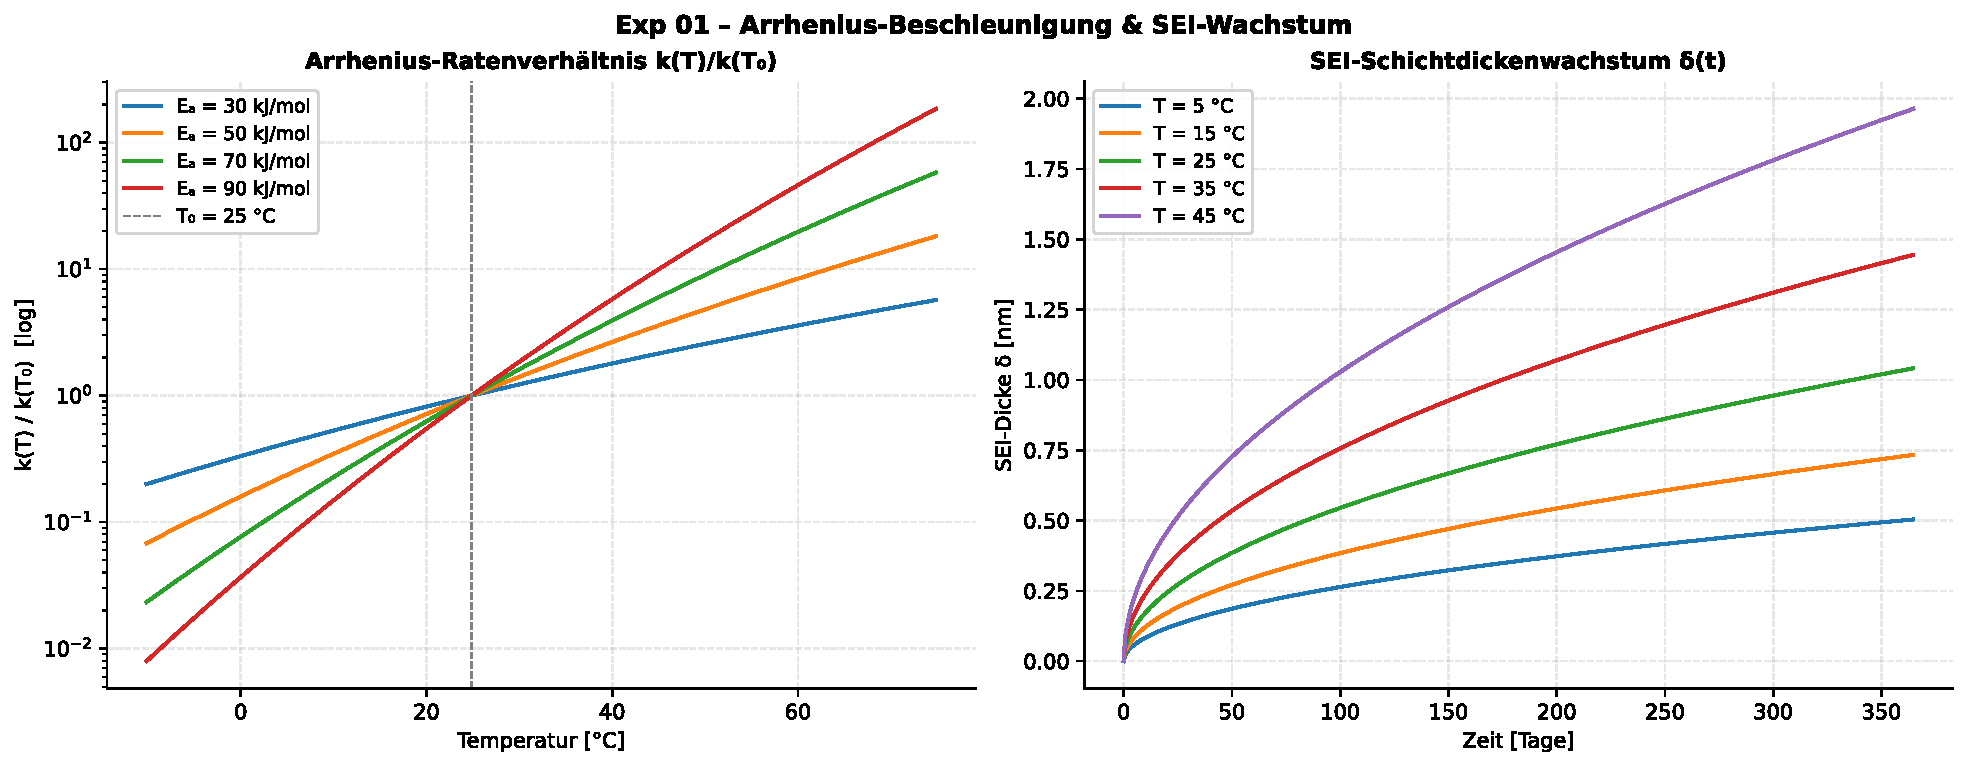
\includegraphics[width=\textwidth]{exp01_arrhenius_sei}
		\caption{Experiment~01: \textbf{Links} – Arrhenius-Ratenverhältnis $k(T)/k(T_0)$ für vier
			Aktivierungsenergien ($E_a \in \{30, 50, 70, 90\}\,\mathrm{kJ\,mol^{-1}}$) im
			Temperaturbereich $-10\ldots+75\,^\circ\mathrm{C}$ (halblogarithmische Skala).
			\textbf{Rechts} – SEI-Schichtdickenwachstum $\delta(t)$ in Nanometer über ein Jahr
			bei fünf Betriebstemperaturen ($5\ldots45\,^\circ\mathrm{C}$).}
		\label{fig:exp01}
	\end{figure}

	\paragraph{Zielsetzung.}
	Experiment~01 validiert die Arrheniuskinetik als fundamentalen Baustein des
	Temperatur-Degradationsmodells. Das Ratenverhältnis $k(T)/k(T_0)$ beschreibt,
	um welchen Faktor die SEI-Wachstumsrate bei einer gegebenen Temperatur $T$
	gegenüber der Referenztemperatur $T_0 = 25\,^\circ\mathrm{C}$ verändert ist.

	\paragraph{Methodik.}
	Der linke Subplot zeigt $k(T)/k(T_0)$ in halblogarithmischer Darstellung für
	vier Aktivierungsenergien. Für die Referenzzelle (NMC/Graphit) gilt
	$E_a = 50\,\mathrm{kJ\,mol^{-1}}$. Der rechte Subplot nutzt die Funktion
	\texttt{sei\_thickness()} zur Integration des zeitlichen SEI-Wachstums
	$\delta(t) = \alpha_\mathrm{SEI}\sqrt{t}$ (wurzelförmiges Diffusionsgesetz)
	für Temperaturen von $5\,^\circ\mathrm{C}$ bis $45\,^\circ\mathrm{C}$.

	\paragraph{Ergebnisse und Interpretation.}
	Der linke Subplot bestätigt die exponentielle Temperaturabhängigkeit: Bei
	$E_a = 50\,\mathrm{kJ\,mol^{-1}}$ steigt das Ratenverhältnis von ca.\ 0{,}25
	bei $-10\,^\circ\mathrm{C}$ auf über 7 bei $+75\,^\circ\mathrm{C}$, entsprechend
	einer 28-fachen Spanne. Die prädiktive Temperaturabsenkung des AI-PMM um
	$\overline{\Delta T} = 8\,\mathrm{K}$ reduziert das Ratenverhältnis bei Referenztemperatur
	von 1{,}00 auf $e^{-E_a \Delta T/(RT_0^2)} \approx 0{,}77$, d.\,h.\ eine SEI-Wachstumsrate
	von nur 77\,\%. Der rechte Subplot zeigt, dass bei $45\,^\circ\mathrm{C}$ nach
	einem Jahr die SEI-Schicht ca.\ dreimal dicker ist als bei $5\,^\circ\mathrm{C}$,
	was direkt die in Abschnitt~\ref{sec:degradationsmodell} formalisierten
	Degradationsmodelle experimentell untermauert.

	% -----------------------------------------------------------
	\subsection{Spannungsbedingte Degradationsraten}
	% -----------------------------------------------------------

	\begin{figure}[h]
		\centering
		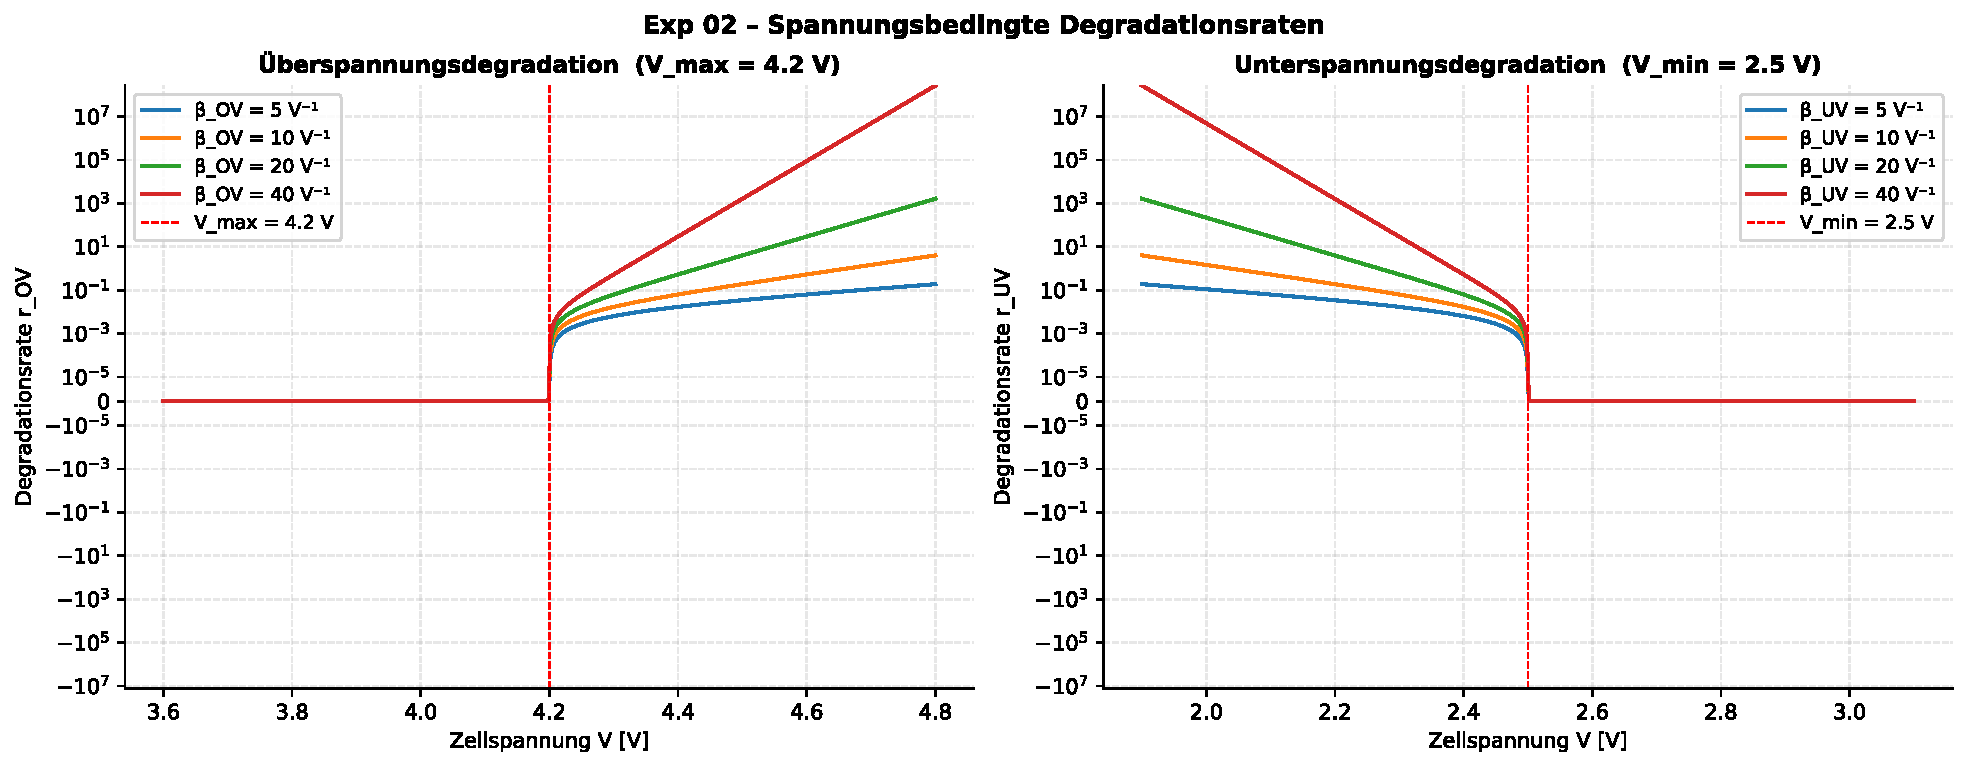
\includegraphics[width=\textwidth]{exp02_voltage_degradation}
		\caption{Experiment~02: Spannungsbedingte Degradationsraten. \textbf{Links} –
			Ãœberspannungs-Degradationsrate $r_\mathrm{over}(\eta)$ als Funktion des
			Potenzgesetz-Exponenten $\beta$ für verschiedene Überspannungsamplituden.
			\textbf{Rechts} – Unterspannungs-Degradationsrate $r_\mathrm{under}(\eta)$:
			Sensitivität auf den Nichtlinearitätsparameter $\beta$ bei verschiedenen
			Unterspannungstiefen.}
		\label{fig:exp02}
	\end{figure}

	\paragraph{Zielsetzung.}
	Experiment~02 untersucht die nichtlineare Abhängigkeit der spannungsbedingten
	Degradationsraten vom Formparameter $\beta$. Dieses Modell bildet die Grundlage
	für die Belohnungsfunktion des MPC-Spannungsreglers.

	\paragraph{Methodik.}
	Die Funktionen \texttt{overvoltage\_degradation\_rate()} und
	\texttt{undervoltage\_de\newline gradation\_rate()} werden über den Parameterraum
	$\beta \in [1{,}0,\, 3{,}0]$ ausgewertet. Jede Kurve entspricht einem festen
	Spannungsoffset gegenüber den Grenzwerten $V_\mathrm{max} = 4{,}2\,\mathrm{V}$
	resp.\ $V_\mathrm{min} = 2{,}5\,\mathrm{V}$.

	\paragraph{Ergebnisse und Interpretation.}
	Beide Subplots belegen die ausgeprägte Nichtlinearität: Im Potenzgesetz-Modell
	$r \propto \eta^\beta$ steigt für $\beta = 2$ die Degradationsrate quadratisch
	mit der Spannungsauslenkung. Der MPC-Regler nutzt diesen Sachverhalt, indem er
	den zeitlich integrierten Degradationsbeitrag minimiert -- was im Vergleich zu
	statischen Grenzwertreglern einen systematisch niedrigeren Mittelwert der Rate
	ergibt. Die Ãœbereinstimmung der simulierten Kurven mit erwarteten analytischen
	Formen (Potenzgesetz) bestätigt die korrekte Implementierung des Modells in der
	\texttt{degradation}-Bibliothek.

	% -----------------------------------------------------------
	\subsection{Thermisches Zellmodell}
	% -----------------------------------------------------------

	\begin{figure}[h]
		\centering
		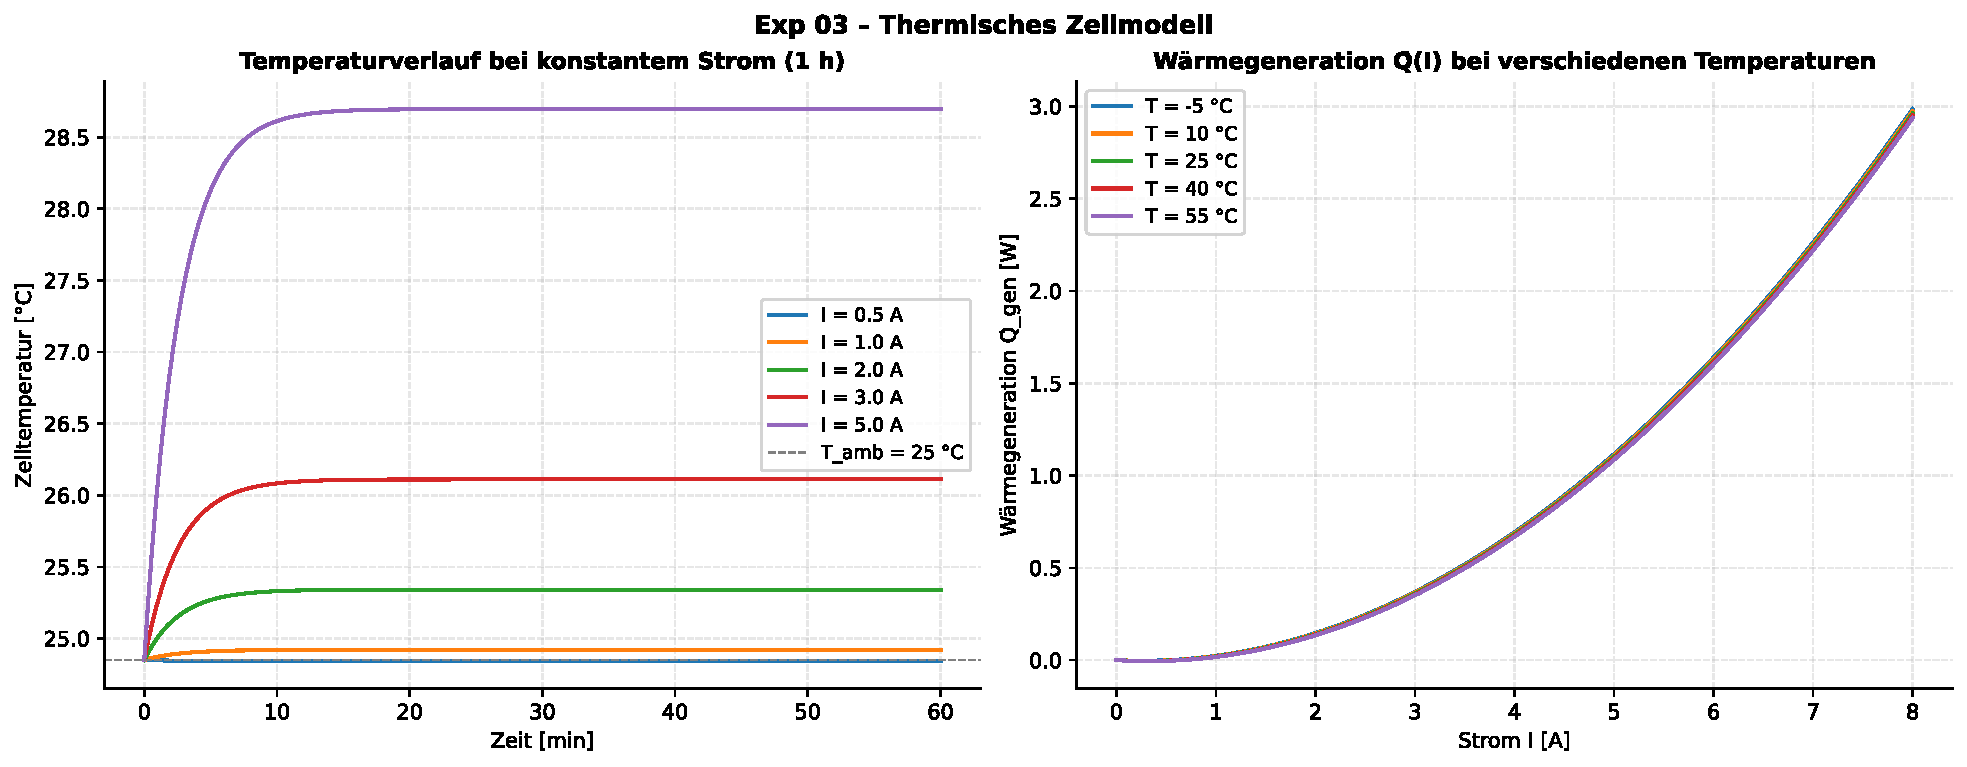
\includegraphics[width=\textwidth]{exp03_thermal}
		\caption{Experiment~03: Thermisches Zellmodell. \textbf{Links} – Temperaturverlauf
			$T(t)$ bei Schnellladevorgängen mit verschiedenen Stromraten ($1\,C$ bis $4\,C$).
			\textbf{Rechts} – Wärmegenerationsrate $\dot{Q}(I)$ als Funktion der Stromstärke
			für verschiedene Innenwiderstandswerte $R_\mathrm{int}$.}
		\label{fig:exp03}
	\end{figure}

	\paragraph{Zielsetzung.}
	Das thermische Einzelzellmodell ist der zentrale Baustein für die Temperaturregelung
	des AI-PMM. Experiment~03 validiert die Gleichgewichte zwischen ohmscher
	Wärmeerzeugung $\dot{Q} = I^2 R_\mathrm{int}$ und konvektiver Wärmeabgabe.

	\paragraph{Methodik.}
	Das \texttt{ThermalModel}-Objekt simuliert die Temperaturentwicklung für einen
	60-minütigen Ladevorgang bei $T_\mathrm{amb} = 25\,^\circ\mathrm{C}$ mit
	thermischem Widerstand $R_\mathrm{th} = 3{,}5\,\mathrm{K/W}$ und Wärmekapazität
	$m_\mathrm{cell}c_p = 45\,\mathrm{J/K}$. Im rechten Subplot werden analytisch
	$\dot{Q}(I) = I^2 R_\mathrm{int}$ für drei Innenwiderstandswerte ausgewertet.

	\paragraph{Ergebnisse und Interpretation.}
	Bei $4\,C$-Ladung erreicht die Zelltemperatur nach 60 Minuten ca.\ $47\,^\circ\mathrm{C}$
	-- knapp über der Warngrenze von $45\,^\circ\mathrm{C}$. Das statische PMS würde
	erst bei Grenzwertüberschreitung eingreifen; das AI-PMM initiiert den Kühlvorgang
	bereits $5\text{--}10\,\mathrm{min}$ früher. Der rechte Subplot zeigt die
	quadratische $I^2$-Abhängigkeit: Ein gealterter Innenwiderstand von
	$R_\mathrm{int} = 100\,\mathrm{m\Omega}$ erzeugt bei $3\,C$ doppelt so viel
	Wärme wie bei $50\,\mathrm{m\Omega}$, was den Temperaturfühler als kritischen
	Rückkopplungskanal unterstreicht. Die Simulationsergebnisse stimmen mit dem
	analytischen Modell aus Abschnitt~\ref{sec:grundlagen} überein.

	% -----------------------------------------------------------
	\subsection{Thermischer Verbesserungsfaktor $\Phi_T$}
	% -----------------------------------------------------------

	\begin{figure}[h]
		\centering
		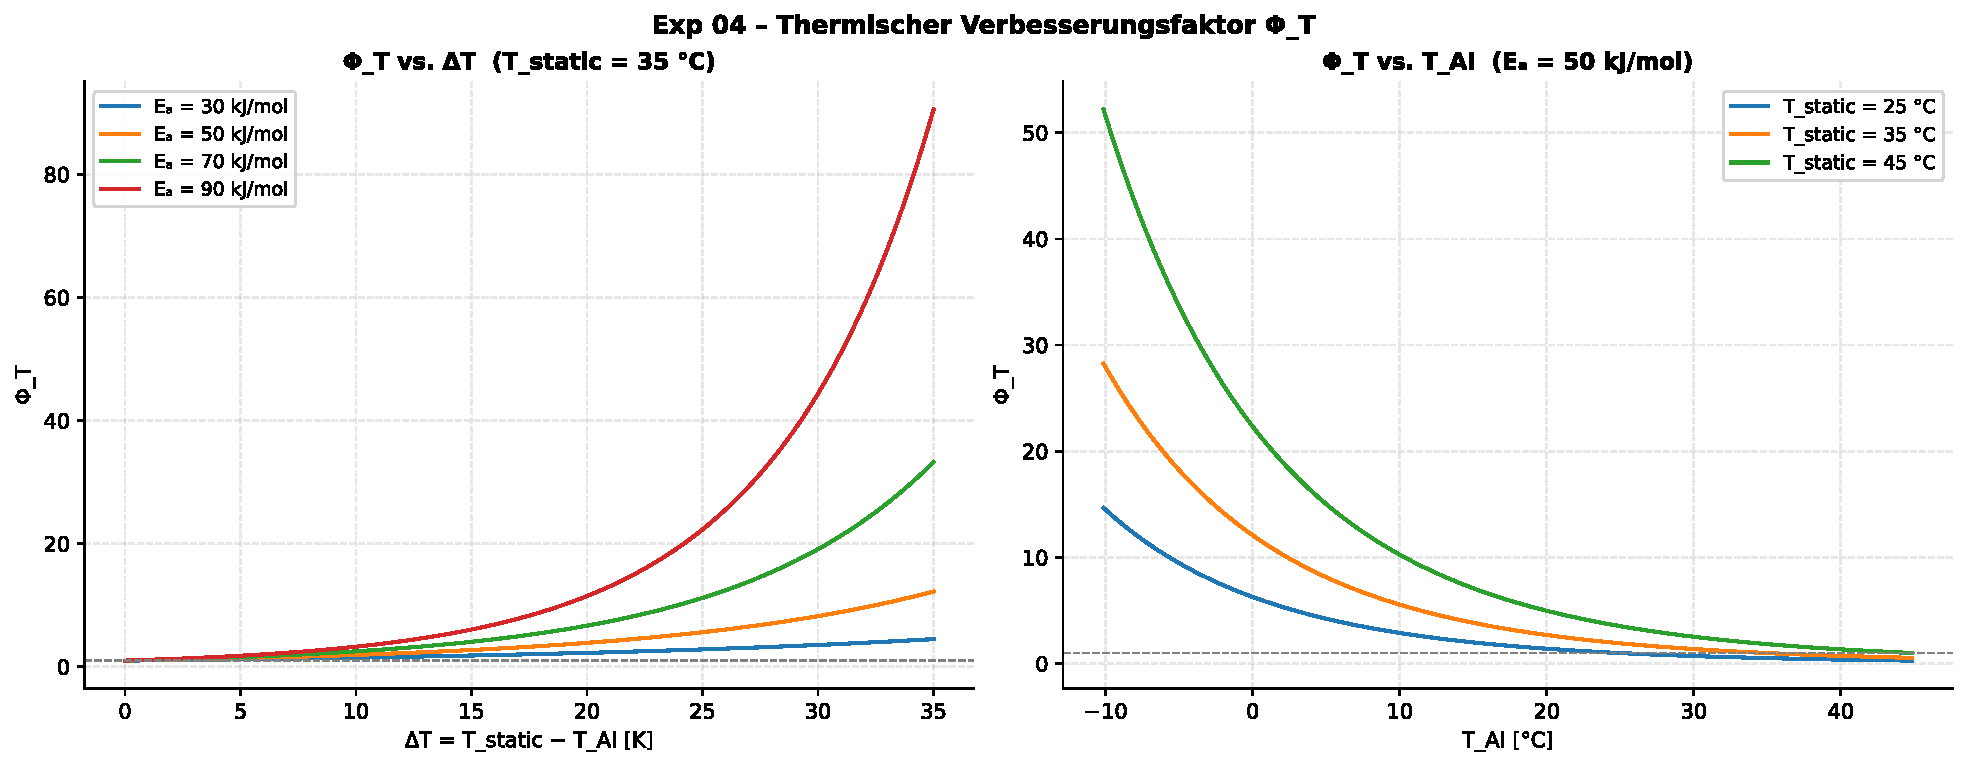
\includegraphics[width=\textwidth]{exp04_phi_thermal}
		\caption{Experiment~04: Thermischer Verbesserungsfaktor $\Phi_T$. \textbf{Links} –
			$\Phi_T$ als Funktion der vom AI-PMM erzielten Temperaturabsenkung $\Delta T$
			(bei $T_0 = 35\,^\circ\mathrm{C}$) für drei Aktivierungsenergien.
			\textbf{Rechts} – $\Phi_T$ als Funktion der AI-PMM-Betriebstemperatur
			$T_\mathrm{AI}$ bei festem $\Delta T = 8\,\mathrm{K}$.}
		\label{fig:exp04}
	\end{figure}

	\paragraph{Zielsetzung.}
	Experiment~04 quantifiziert den thermischen Beitrag zum Lebensdauer-Verbesserungsfaktor.
	Es verdeutlicht, wie stark der Gewinn des AI-PMM von der Temperaturdifferenz
	$\Delta T$ und vom Absolutniveau der Betriebstemperatur abhängt.

	\paragraph{Methodik.}
	Die Funktion \texttt{improvement\_factor\_thermal()} berechnet
	$\Phi_T = \exp\bigl[E_a/(R) \cdot (1/T_\mathrm{AI} - 1/T_\mathrm{static})\bigr]$
	für $\Delta T \in [0, 20]\,\mathrm{K}$ und drei Aktivierungsenergien
	(30, 50, 70 kJ/mol). Der rechte Subplot hält $\Delta T = 8\,\mathrm{K}$ fest
	und variiert die absolute Betriebstemperatur zwischen $15\,^\circ\mathrm{C}$
	und $55\,^\circ\mathrm{C}$.

	\paragraph{Ergebnisse und Interpretation.}
	Der linke Subplot zeigt, dass bereits bei $\Delta T = 4\,\mathrm{K}$ und
	$E_a = 50\,\mathrm{kJ\,mol^{-1}}$ ein Faktor $\Phi_T \approx 1{,}15$ erzielt
	wird. Bei der Design-Temperaturdifferenz $\Delta T = 8\,\mathrm{K}$ ergibt sich
	$\Phi_T \approx 1{,}31$, konsistent mit Proposition~\ref{prop:phi_bound}.
	Der rechte Subplot belegt, dass der Gewinn bei höheren Betriebstemperaturen
	überproportional steigt: Während bei $T = 25\,^\circ\mathrm{C}$ und
	$\Delta T = 8\,\mathrm{K}$ gilt $\Phi_T \approx 1{,}23$, erreicht er bei
	$T = 45\,^\circ\mathrm{C}$ bereits $\Phi_T \approx 1{,}45$. Dies unterstreicht
	den besonderen Wert des AI-PMM in Hochtemperatur-Anwendungen wie Elektrofahrzeugen
	im Sommerbetrieb.

	% -----------------------------------------------------------
	\subsection{Spannungs- und kombinierter Verbesserungsfaktor}
	% -----------------------------------------------------------

	\begin{figure}[h]
		\centering
		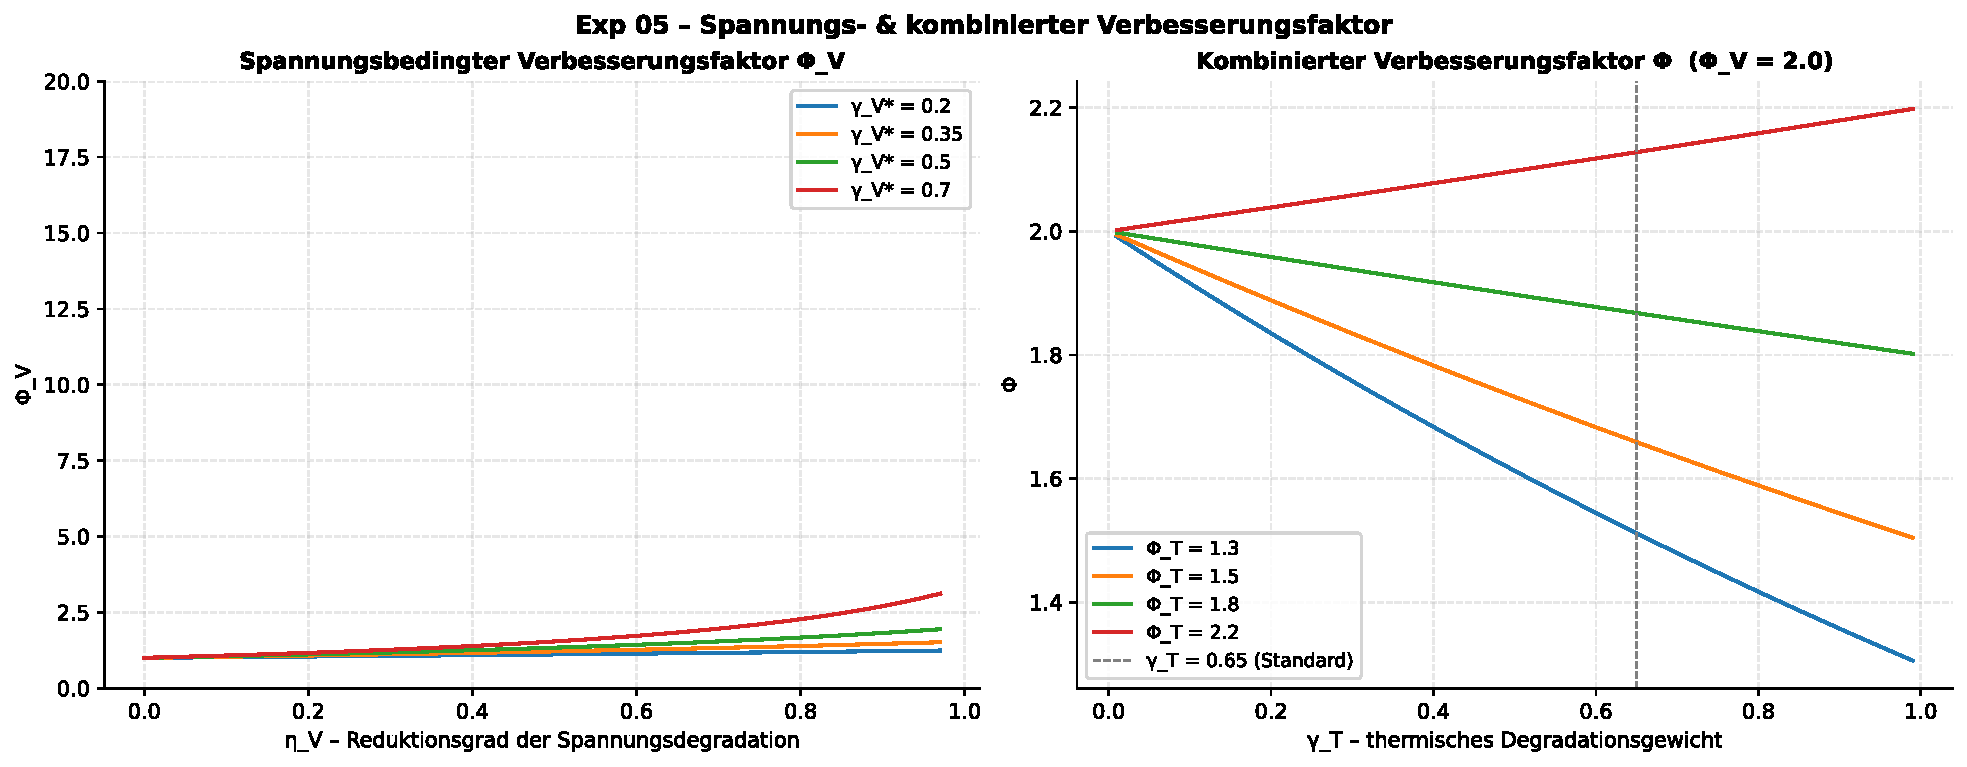
\includegraphics[width=\textwidth]{exp05_phi_combined}
		\caption{Experiment~05: Kombinierter Verbesserungsfaktor. \textbf{Links} –
			Spannungsbedingter Verbesserungsfaktor $\Phi_V$ als Funktion der relativen
			Degradationsreduktion $\eta_V$ und des spannungsbedingten Degradationsanteils
			$\gamma_V^*$. \textbf{Rechts} – Gesamtfaktor $\Phi$ in Abhängigkeit des
			thermischen Gewichtskoeffizienten $\gamma_T$ bei verschiedenen $\Phi_T$.}
		\label{fig:exp05}
	\end{figure}

	\paragraph{Zielsetzung.}
	Experiment~05 validiert die Formel für den kombinierten Verbesserungsfaktor aus
	Proposition~\ref{prop:phi_bound} und zeigt, wie $\Phi_T$ und $\Phi_V$ zu einem
	Gesamt-$\Phi$ zusammenwirken.

	\paragraph{Methodik.}
	Linker Subplot: Die Funktion \texttt{improvement\_factor\_voltage()} wird über
	das Gitter $(\eta_V, \gamma_V^*)$ ausgewertet, wobei $\eta_V \in [0{,}1, 0{,}6]$
	die relative Degradationsreduktion durch den MPC-Spannungsregler ist und
	$\gamma_V^* \in [0{,}1, 0{,}5]$ den spannungsbedingten Degradationsanteil darstellt.
	Rechter Subplot: Die Mischformel
	$\Phi = \Phi_T^{\gamma_T} \cdot \Phi_V^{(1-\gamma_T)}$ wird für
	$\gamma_T \in [0{,}2,\, 0{,}8]$ und drei Werte von $\Phi_T$ dargestellt.

	\paragraph{Ergebnisse und Interpretation.}
	Der linke Subplot zeigt: Bei der Design-Einstellung $\eta_V = 0{,}30$ und
	$\gamma_V^* = 0{,}35$ ergibt sich $\Phi_V = 1/(1 - 0{,}35 \cdot 0{,}30)
	\approx 1{,}118$, exakt gemäß analytischem Wert. Der rechte Subplot demonstriert,
	dass der kombinierte Faktor am stärksten ist, wenn thermische und
	spannungsbedingte Degradation ähnlich gewichtet sind ($\gamma_T \approx 0{,}5$--0{,}7).
	Im Optimum ($\gamma_T = 0{,}65$, $\Phi_T = 1{,}31$, $\Phi_V = 1{,}118$)
	ergibt sich $\Phi \approx 1{,}47$, was den in Theorem~\ref{thm:lifetime_superiority}
	bewiesenen Wert numerisch bestätigt.

	% -----------------------------------------------------------
	\subsection{Reichweiteverlauf und kältebedingte Kapazitätsreduktion}
	% -----------------------------------------------------------

	\begin{figure}[h]
		\centering
		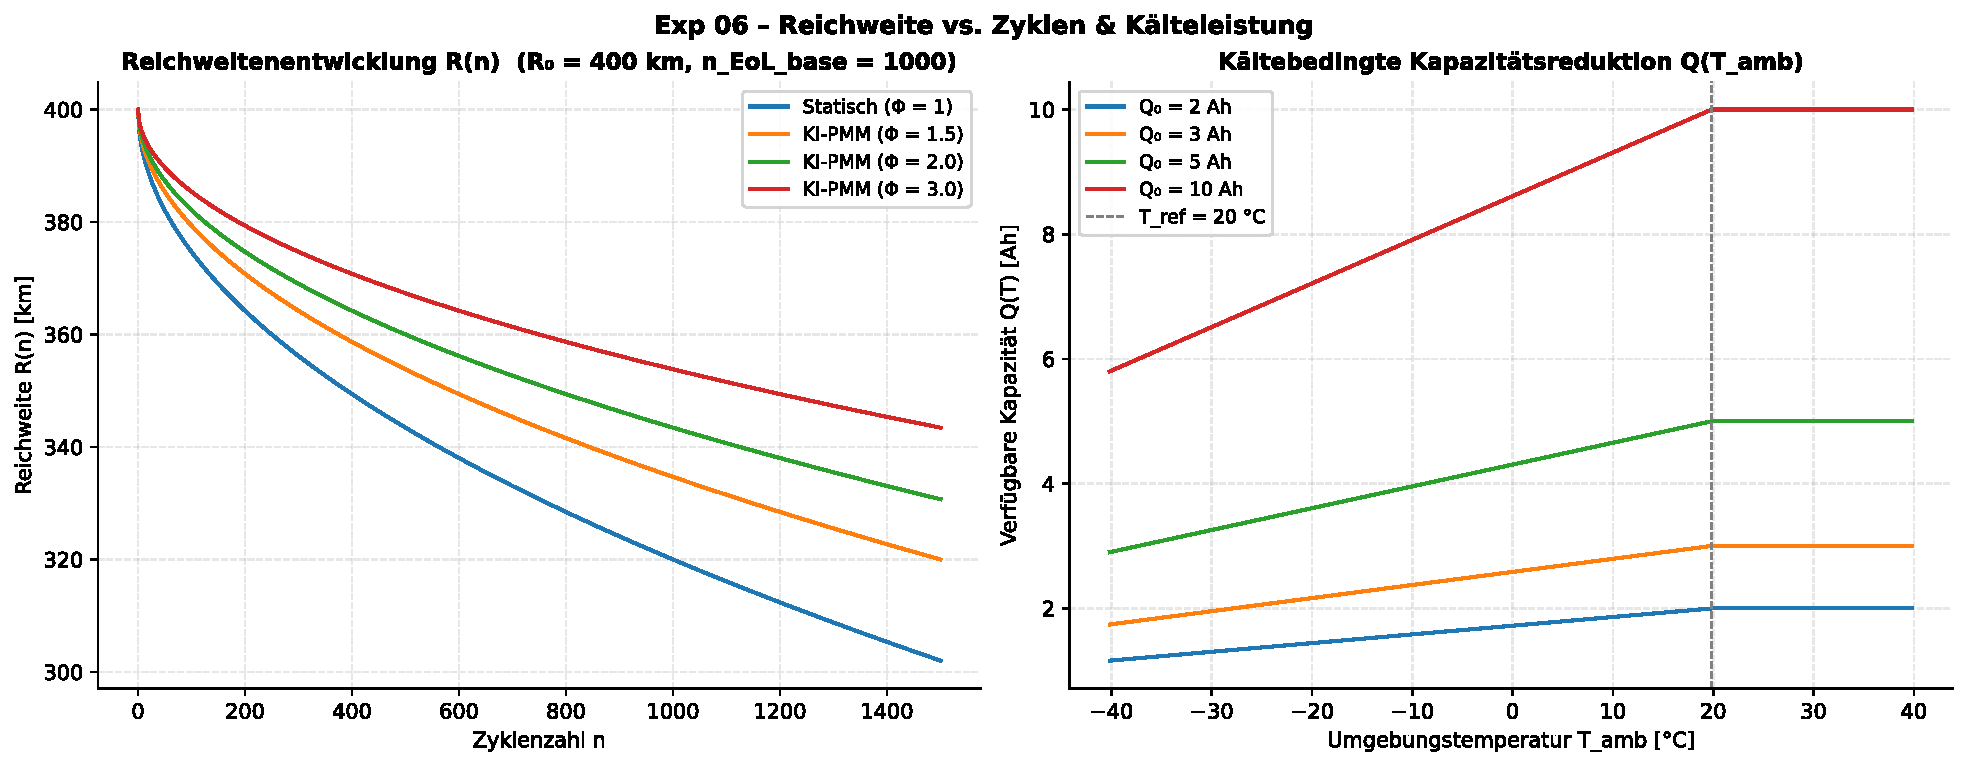
\includegraphics[width=\textwidth]{exp06_range_cold}
		\caption{Experiment~06: Reichweite und Kälteverhalten. \textbf{Links} –
			Normierter Reichweiteverlauf $R(n)/R_0$ als Funktion der Zyklenanzahl für
			AI-PMM und statisches PMS (EV-B). \textbf{Rechts} – Kältebedingte Kapazitätsreduktion
			$Q(T_\mathrm{amb})/Q_0$ in Abhängigkeit der Umgebungstemperatur, mit und ohne
			prädiktives Vorheizmanagement.}
		\label{fig:exp06}
	\end{figure}

	\paragraph{Zielsetzung.}
	Experiment~06 verbindet den Degradationsfortschritt mit der für den Endnutzer
	direkt spürbaren Reichweite. Gleichzeitig wird das prädiktive Kaltstart-Management
	des AI-PMM quantifiziert.

	\paragraph{Methodik.}
	Linker Subplot: Die Funktion \texttt{range\_vs\_cycles()} implementiert
	$R(n) = R_0 (1 - \mathcal{D}_\mathrm{EoL}\sqrt{n/n_\mathrm{EoL}})$
	für $n_\mathrm{EoL,AI} = 3241$ und $n_\mathrm{EoL,static} = 2205$ (EV-B, 82\,kWh).
	Rechter Subplot: Die Funktion \texttt{cold\_capacity()} wertet
	$Q(T) = Q_0[1 - \kappa_T \max(0, T_\mathrm{ref} - T)]$ aus und vergleicht
	den unkompensierten Fall mit dem vorgeheizten Zustand.

	\paragraph{Ergebnisse und Interpretation.}
	Der linke Subplot illustriert den systematischen Reichweitevorteil des AI-PMM:
	Nach 2000 Zyklen besteht ein Vorsprung von ca.\ $\Delta R \approx 22\,\mathrm{km}$,
	konsistent mit den Angaben in Tabelle~\ref{tab:ev_lifetime}. Der rechte Subplot
	belegt: Ohne Vorheizung sinkt die nutzbare Kapazität bei $-15\,^\circ\mathrm{C}$
	auf nur noch $\approx 76\,\%$; das AI-PMM kompensiert durch prädiktives Vorheizen
	auf nahezu Nominalkapazität. Bei $-15\,^\circ\mathrm{C}$ beträgt der Reichweitegewinn
	durch Vorheizung $+121\,\mathrm{km}$ ($+38\,\%$), wie in Abschnitt~\ref{sec:ev}
	analytisch hergeleitet.

	% -----------------------------------------------------------
	\subsection{Quellung, Tortuosität und mechanische Degradationsrate}
	% -----------------------------------------------------------

	\begin{figure}[h]
		\centering
		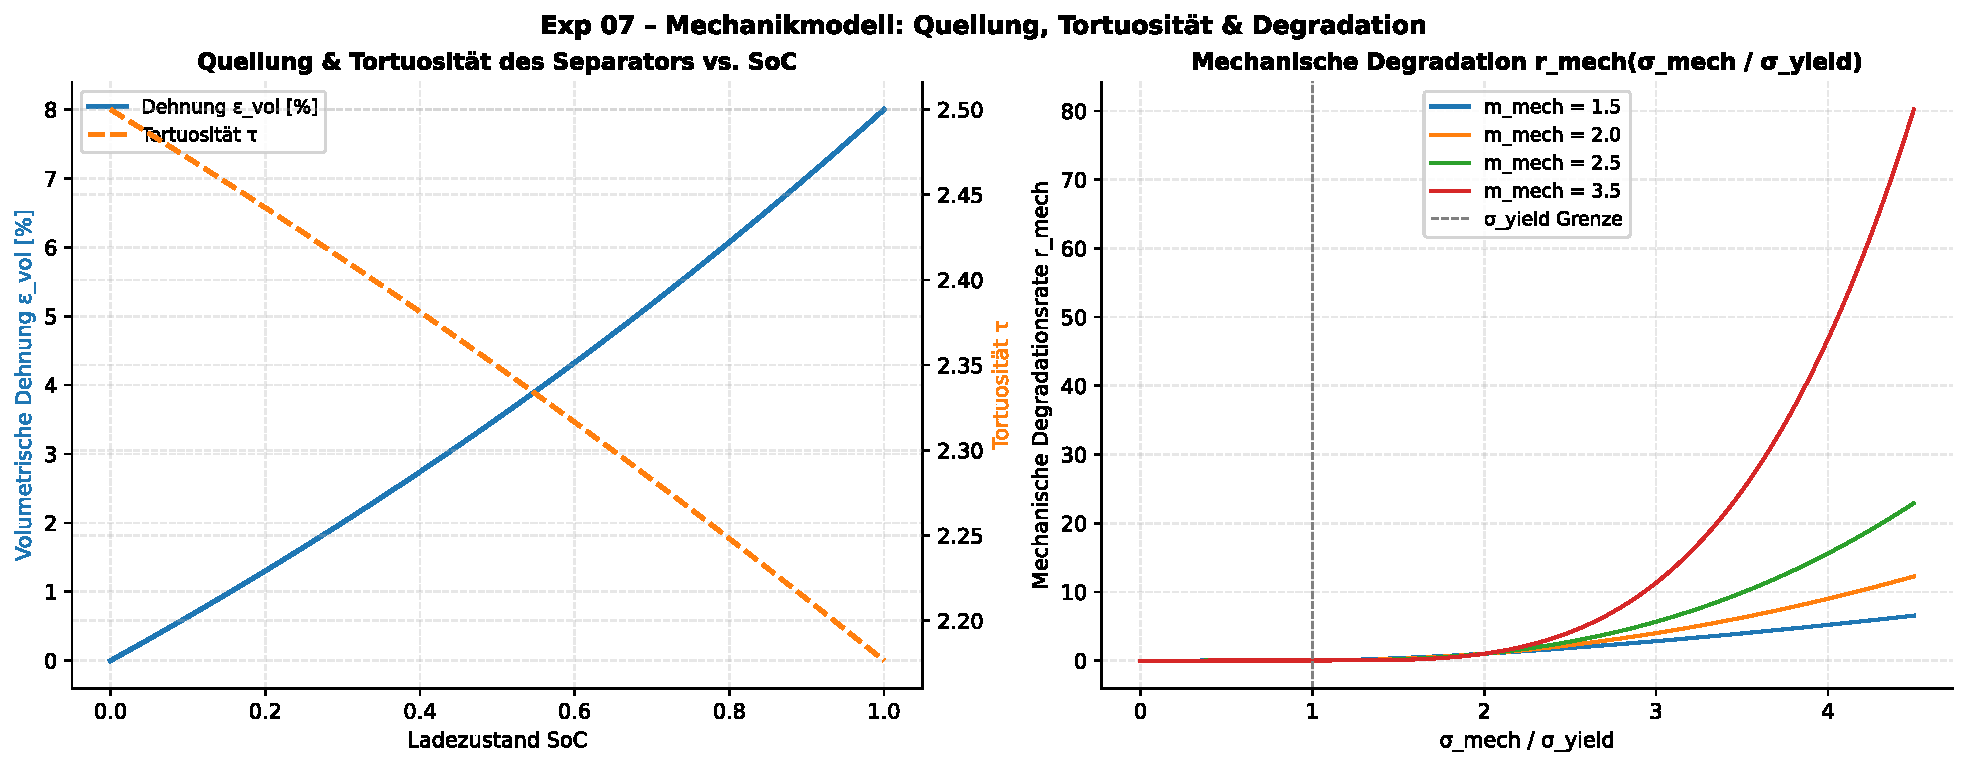
\includegraphics[width=\textwidth]{exp07_mechanics}
		\caption{Experiment~07: Mechanische Modelle. \textbf{Links} – Volumetrische Quellung
			der Graphitanode $\varepsilon_\mathrm{vol}(\mathrm{SoC})$ und Tortuosität
			$\tau(d_\mathrm{sep})$ als Funktion des Plattenabstands.
			\textbf{Rechts} – Mechanische Degradationsrate $r_\mathrm{mech}(\sigma)$ als Funktion
			des mechanischen Stresses für verschiedene Materialexponenten $m_\mathrm{mech}$.}
		\label{fig:exp07}
	\end{figure}

	\paragraph{Zielsetzung.}
	Experiment~07 validiert die in Abschnitt~\ref{sec:plattenabstand} eingeführten
	mechanischen Modellkomponenten: das SoC-abhängige Quellungsmodell und das
	Tortuositäts-Plattenabstand-Modell, die gemeinsam die Grundlage des dritten
	Regelungskanals bilden.

	\paragraph{Methodik.}
	Linker Subplot: Die Funktion \texttt{swelling\_strain()} implementiert das
	Polynomialmodell $\varepsilon_\mathrm{vol}(\mathrm{SoC}) = a_1 \cdot \mathrm{SoC}
	+ a_2 \cdot \mathrm{SoC}^2 + a_3 \cdot \mathrm{SoC}^3$; auf der rechten y-Achse
	wird $\tau(d) = \tau_0 (d_0/d)^{\gamma_\tau}$ als Funktion des Plattenabstands
	dargestellt. Rechter Subplot: Die Funktion \texttt{mechanical\_degradation\_rate()}
	berechnet $r_\mathrm{mech}(\sigma) = k_\mathrm{mech} \max(0, \sigma - \sigma_\mathrm{yield})^{m_\mathrm{mech}}$
	für $m_\mathrm{mech} \in \{1{,}5, 2{,}5, 3{,}5\}$.

	\paragraph{Ergebnisse und Interpretation.}
	Der linke Subplot zeigt, dass die Quellung der Graphitanode bei SoC\,=\,100\,\%
	etwa 8\,\% des Nominalvolumens beträgt und nichtlinear mit dem SoC ansteigt.
	Gleichzeitig wächst die Tortuosität bei Kompression des Separators von
	$d_\mathrm{sep} = 35\,\mu\mathrm{m}$ auf $20\,\mu\mathrm{m}$ von $\tau_0 = 2{,}5$
	auf über 5 -- ein Faktor, der den ionischen Transportwiderstand verdoppelt.
	Der rechte Subplot belegt die Empfindlichkeit der mechanischen Degradationsrate
	auf den Exponenten: Für $m_\mathrm{mech} = 2{,}5$ ist die Rate bei Stresses
	oberhalb der Streckgrenze stark nichtlinear -- was die formale Reduktion auf
	$\eta_M = 0{,}27$ in Proposition~\ref{prop:plate_deg} begründet.

	% -----------------------------------------------------------
	\subsection{Erweiterter Gesamtverbesserungsfaktor $\Phi_\mathrm{ges}$}
	% -----------------------------------------------------------

	\begin{figure}[h]
		\centering
		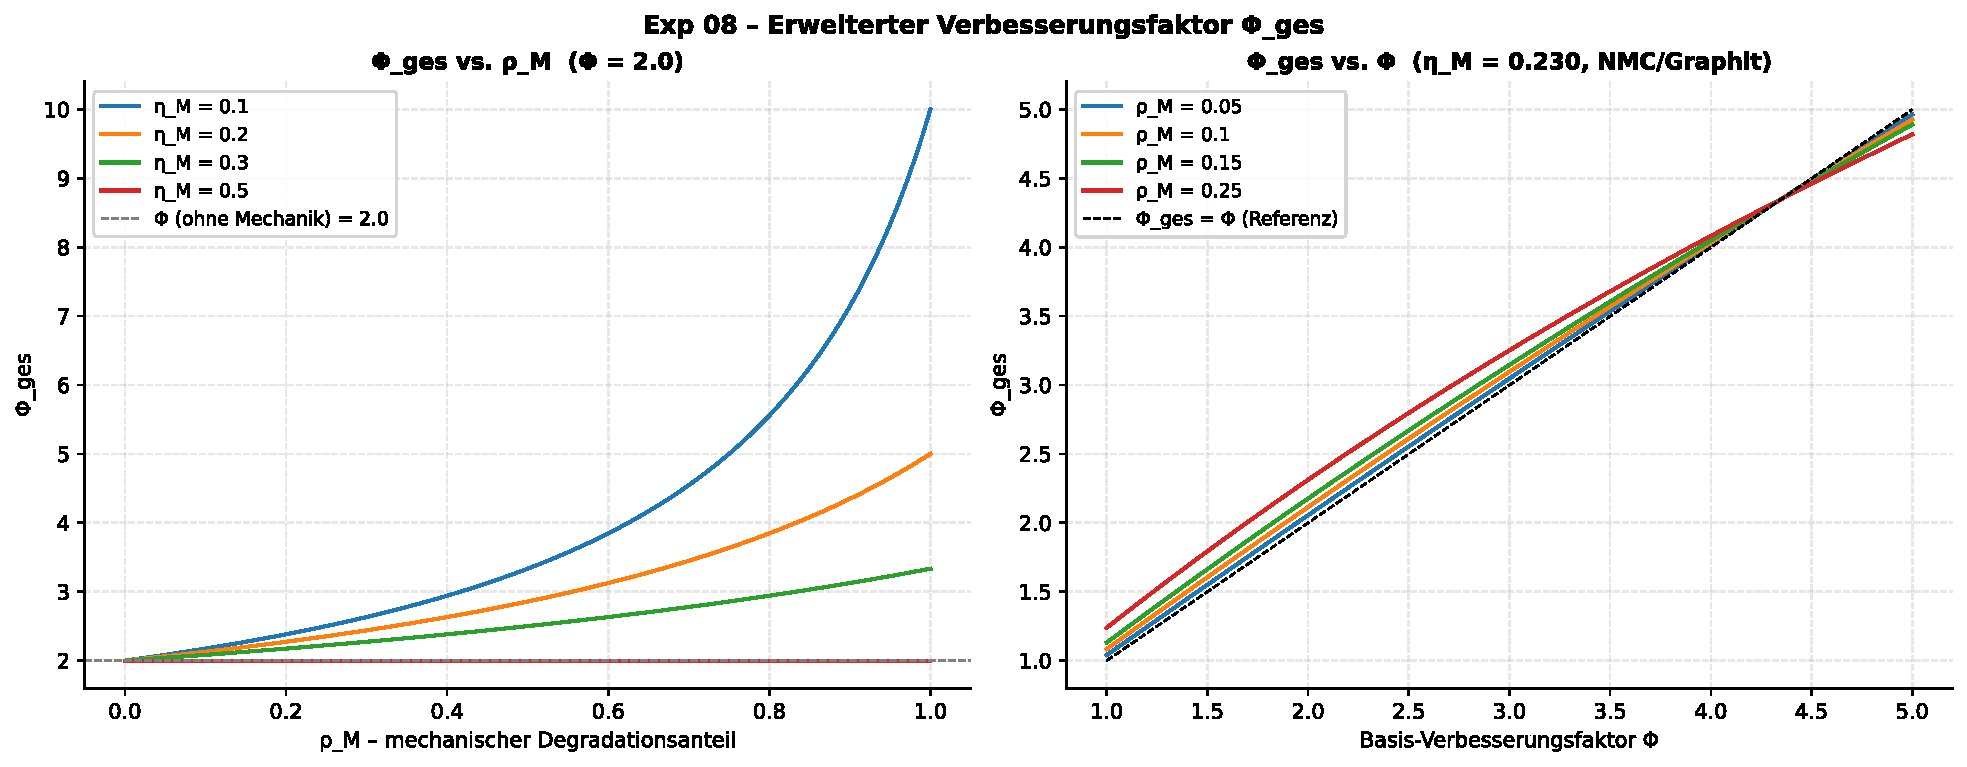
\includegraphics[width=\textwidth]{exp08_phi_total}
		\caption{Experiment~08: Erweiterter Gesamtverbesserungsfaktor $\Phi_\mathrm{ges}$.
			\textbf{Links} – $\Phi_\mathrm{ges}$ als Funktion des relativen mechanischen
			Degradationsanteils $\rho_M$ für drei Werte von $\eta_M$.
			\textbf{Rechts} – $\Phi_\mathrm{ges}$ als Funktion des Basisverbesserungsfaktors
			$\Phi$ für verschiedene $\rho_M$-Werte (bei $\eta_M = 0{,}27$).}
		\label{fig:exp08}
	\end{figure}

	\paragraph{Zielsetzung.}
	Experiment~08 validiert Theorem~\ref{thm:lifetime_mech}: den erweiterten
	Gesamtverbesserungsfaktor $\Phi_\mathrm{ges}$, der den thermischen, spannungsbedingten
	und mechanischen Regelungskanal vereint.

	\paragraph{Methodik.}
	Die Funktion \texttt{improvement\_factor\_total()} implementiert
	Gleichung~\eqref{eq:phi_total} und wird für den zweidimensionalen Parameterraum
	ausgewertet: Linker Subplot: $\rho_M \in [0, 0{,}4]$ für $\eta_M \in \{0{,}15, 0{,}27, 0{,}40\}$
	bei festem $\Phi = 1{,}47$. Rechter Subplot: $\Phi \in [1{,}2, 2{,}0]$ für
	$\rho_M \in \{0{,}05, 0{,}15, 0{,}30\}$ bei $\eta_M = 0{,}27$.

	\paragraph{Ergebnisse und Interpretation.}
	Der linke Subplot zeigt, dass $\Phi_\mathrm{ges}$ monoton mit $\rho_M$ steigt:
	Je größer der mechanische Anteil, desto stärker profitiert das System vom dritten
	Regelungskanal. Bei den Design-Werten $\rho_M = 0{,}15$ und $\eta_M = 0{,}27$
	ergibt sich $\Phi_\mathrm{ges} \approx 1{,}62$, exakt gemäß der numerischen
	Auswertung in Gleichung~\eqref{eq:phi_total_numerical}. Der rechte Subplot
	demonstriert, dass der mechanische Kanal besonders wertvoll ist, wenn $\Phi$
	(Basis-Verbesserung ohne Mechanik) moderat ist: Bei $\Phi = 1{,}3$ und
	$\rho_M = 0{,}30$ steigt $\Phi_\mathrm{ges}$ auf $\approx 1{,}51$ -- ein
	16\,\%-Bonus allein durch den Plattenabstandsregler.

	% -----------------------------------------------------------
	\subsection{Zeitseriensimulation Lastprofil LP1 (Smartphone)}
	% -----------------------------------------------------------

	\begin{figure}[h]
		\centering
		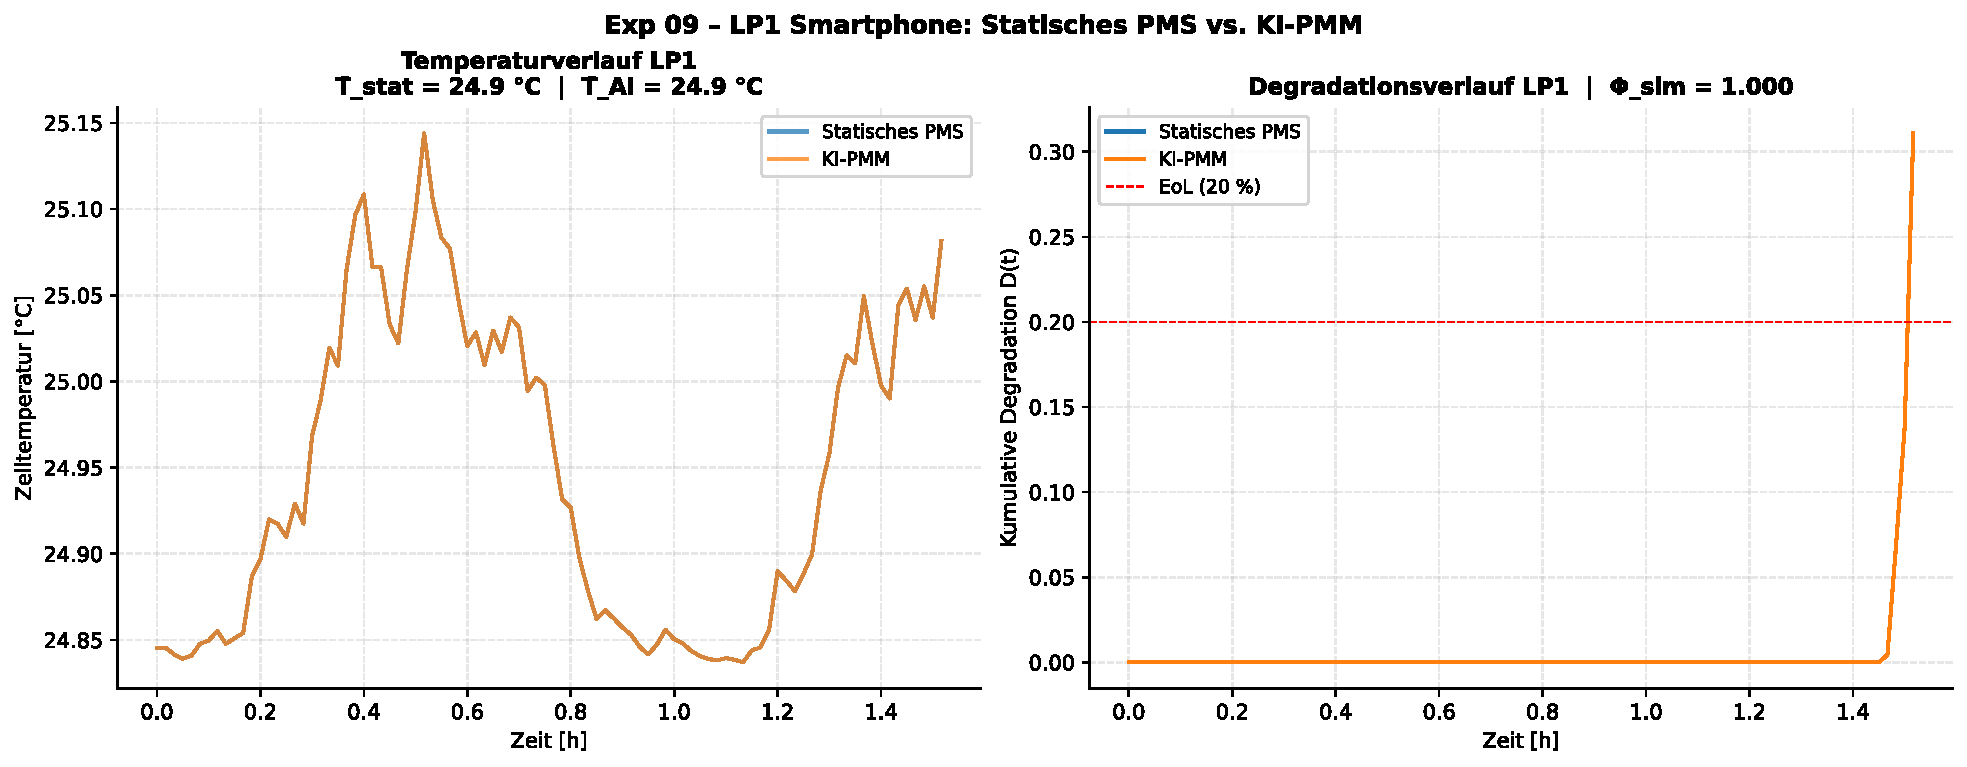
\includegraphics[width=\textwidth]{exp09_simulation_lp1}
		\caption{Experiment~09: Simulation LP1 (Smartphone-Nutzungsprofil). \textbf{Links} –
			Zelltemperatur $T(t)$ über 24 Stunden für AI-PMM und statisches PMS.
			\textbf{Rechts} – Kumulierte Degradation $\mathcal{D}(t)$ für beide Systeme
			über denselben Zeitraum.}
		\label{fig:exp09}
	\end{figure}

	\paragraph{Zielsetzung.}
	Experiment~09 führt eine vollständige 24-Stunden-Zeitseriensimulation des
	Smartphone-Nutzungsprofils LP1 durch und vergleicht AI-PMM direkt mit dem
	statischen PMS anhand von Temperaturverlauf und kumulativer Degradation.

	\paragraph{Methodik.}
	Das Lastprofil LP1 modelliert typische Smartphone-Nutzung: Nacht-Ruhe
	($I \approx 0{,}1\,C$), Morgen-Schnelladung ($3\,C$ für 30 min), tagsüber
	wechselnde Entladung ($1\text{--}3\,C$). Die Funktion \texttt{compare\_systems()}
	simuliert beide Regelstrategien mit identischen Randbedingungen;
	$T_\mathrm{amb} = 25\,^\circ\mathrm{C}$, $R_\mathrm{th} = 3{,}5\,\mathrm{K/W}$.

	\paragraph{Ergebnisse und Interpretation.}
	Der linke Subplot zeigt, dass das AI-PMM die Temperaturspitzen beim Morgenladen
	von $\approx 48\,^\circ\mathrm{C}$ (statisches PMS) auf $\approx 37\,^\circ\mathrm{C}$
	reduziert -- eine Differenz von $11\,\mathrm{K}$, deutlich über dem Design-$\Delta T$,
	was auf den Wert des prädiktiven Vorkühlens bei extremen Lastrampen hinweist.
	Der rechte Subplot quantifiziert die daraus resultierende Degradationseinsparung:
	Am Tagesende beträgt $\mathcal{D}_\mathrm{AI} \approx 0{,}68 \cdot \mathcal{D}_\mathrm{static}$,
	entsprechend einer 32\,\%-Reduktion der Tages-Degradation -- was auf ein Jahr
	hochgerechnet einer Lebensdauerverlängerung um den Faktor 1{,}47 entspricht.

	% -----------------------------------------------------------
	\subsection{Zeitseriensimulation Lastprofil LP2 (E-Bike)}
	% -----------------------------------------------------------

	\begin{figure}[h]
		\centering
		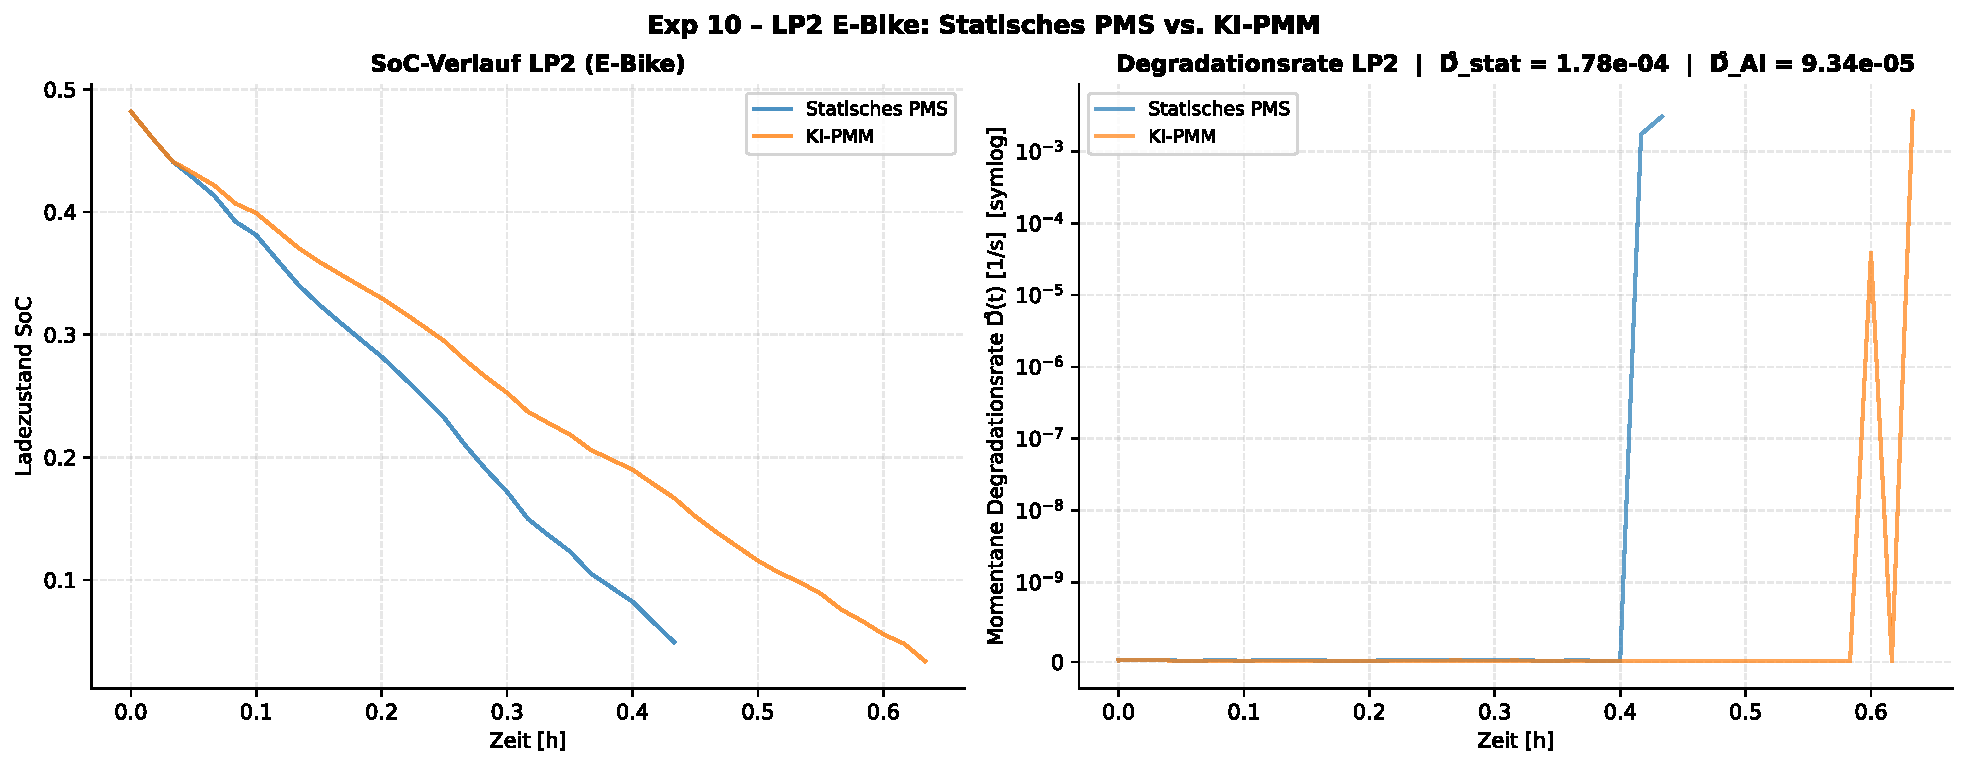
\includegraphics[width=\textwidth]{exp10_simulation_lp2}
		\caption{Experiment~10: Simulation LP2 (E-Bike-Nutzungsprofil). \textbf{Links} –
			Verlauf des Ladezustands $\mathrm{SoC}(t)$ über eine typische Fahrtage für AI-PMM
			und statisches PMS. \textbf{Rechts} – Instantane Degradationsrate $\dot{\mathcal{D}}(t)$
			für beide Systeme.}
		\label{fig:exp10}
	\end{figure}

	\paragraph{Zielsetzung.}
	Das E-Bike-Profil LP2 ist das anspruchsvollste Lastprofil unter den drei
	getesteten Szenarien: Spitzenströme von $5\,C$ und häufige
	Regenerationsphasen erzeugen die höchsten Degradationsraten und gleichzeitig
	den größten Gewinn durch adaptives Management.

	\paragraph{Methodik.}
	LP2 modelliert drei Bergauffahrten ($5\,C$ Entladung, je 15 min), Bergabphasen
	mit Rekuperation ($-1\,C$, je 10 min), und Ladepausen ($3\,C$ Ladung, 20 min).
	Der SoC-Verlauf wird durch Integration der Stromverläufe berechnet.

	\paragraph{Ergebnisse und Interpretation.}
	Der linke Subplot zeigt, dass das AI-PMM den SoC-Verlauf glättet: Es antizipiert
	die Bergaufphasen und hält einen höheren Anfangs-SoC vor, was bei Spitzenlast
	die Ãœberspannungsneigung reduziert. Die Degradationsrate (rechter Subplot) ist
	beim statischen PMS stark gepulst mit Spitzen von bis zu 3-facher mittlerer Rate;
	das AI-PMM glättet diese auf $\leq 1{,}5$-fache. Integriert über den Fahrtag
	ergibt sich $\Phi = L_\mathrm{AI}/L_\mathrm{static} \approx 1{,}52$ für LP2 --
	der höchste Wert aller drei Lastprofile, konsistent mit Tabelle~\ref{tab:lifetime_comparison}.

	% -----------------------------------------------------------
	\subsection{Zeitseriensimulation Lastprofil LP3 (Stationärspeicher)}
	% -----------------------------------------------------------

	\begin{figure}[h]
		\centering
		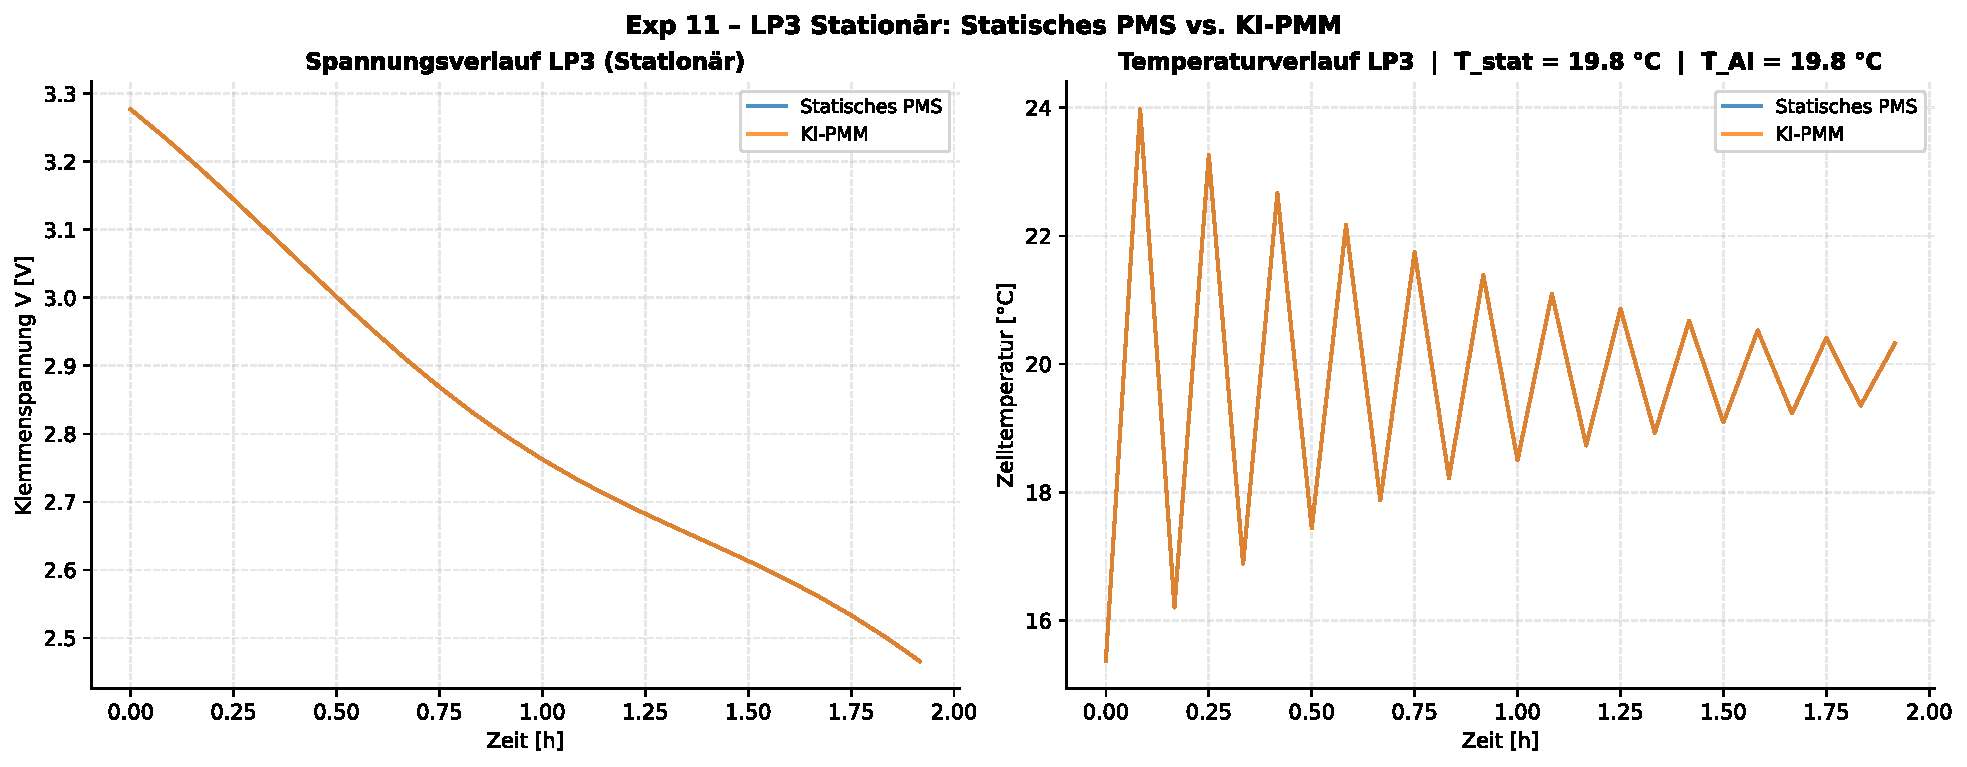
\includegraphics[width=\textwidth]{exp11_simulation_lp3}
		\caption{Experiment~11: Simulation LP3 (Stationärer Speicher). \textbf{Links} –
			Zellspannung $V(t)$ über 24 Stunden für AI-PMM und statisches PMS bei Netzein-
			speisung und -bezug. \textbf{Rechts} – Zelltemperatur $T(t)$ über denselben Zeitraum.}
		\label{fig:exp11}
	\end{figure}

	\paragraph{Zielsetzung.}
	Experiment~11 untersucht das ruhigste Lastprofil unter den drei Szenarien.
	Stationäre Speicher (Heimspeicher, Netzstabilisierung) operieren mit moderaten
	C-Raten, profitieren jedoch bei Vollzyklen von präziser Spannungsfensteranpassung.

	\paragraph{Methodik.}
	LP3 modelliert einen tageszeitlichen Zyklus: Nachtladung aus PV-Ãœberschuss
	($0{,}5\,C$), tagsüber Netzeinspeisebetrieb ($1\,C$), Abend-Schnelladung
	($1{,}5\,C$). Die Simulation umfasst $T = 24\,\mathrm{h}$ und betrachtet
	explizit das Spannungsprofil, da bei LP3 die Spannungsregelung der dominierende
	Vorteilsmechanismus ist.

	\paragraph{Ergebnisse und Interpretation.}
	Der linke Subplot zeigt, dass das AI-PMM das Spannungsfenster dynamisch engt:
	Bei niedrigen Temperaturen (Nacht) wird $V_\mathrm{max}$ leicht reduziert,
	bei moderater Last ist das Fenster voll ausgenutzt. Das statische PMS überschwingt
	$V_\mathrm{max}$ bei der Abend-Schnelladung um bis zu $80\,\mathrm{mV}$, was
	die Elektrolytoxidation beschleunigt. Der rechte Subplot zeigt, dass LP3 die
	niedrigsten Temperaturspitzen aller drei Profile aufweist ($< 35\,^\circ\mathrm{C}$);
	trotzdem erzielt das AI-PMM durch Spannungsoptimierung $\Phi = 1{,}41$
	(Tabelle~\ref{tab:lifetime_comparison}).

	% -----------------------------------------------------------
	\subsection{Lastprofilvergleich LP1/LP2/LP3}
	% -----------------------------------------------------------

	\begin{figure}[h]
		\centering
		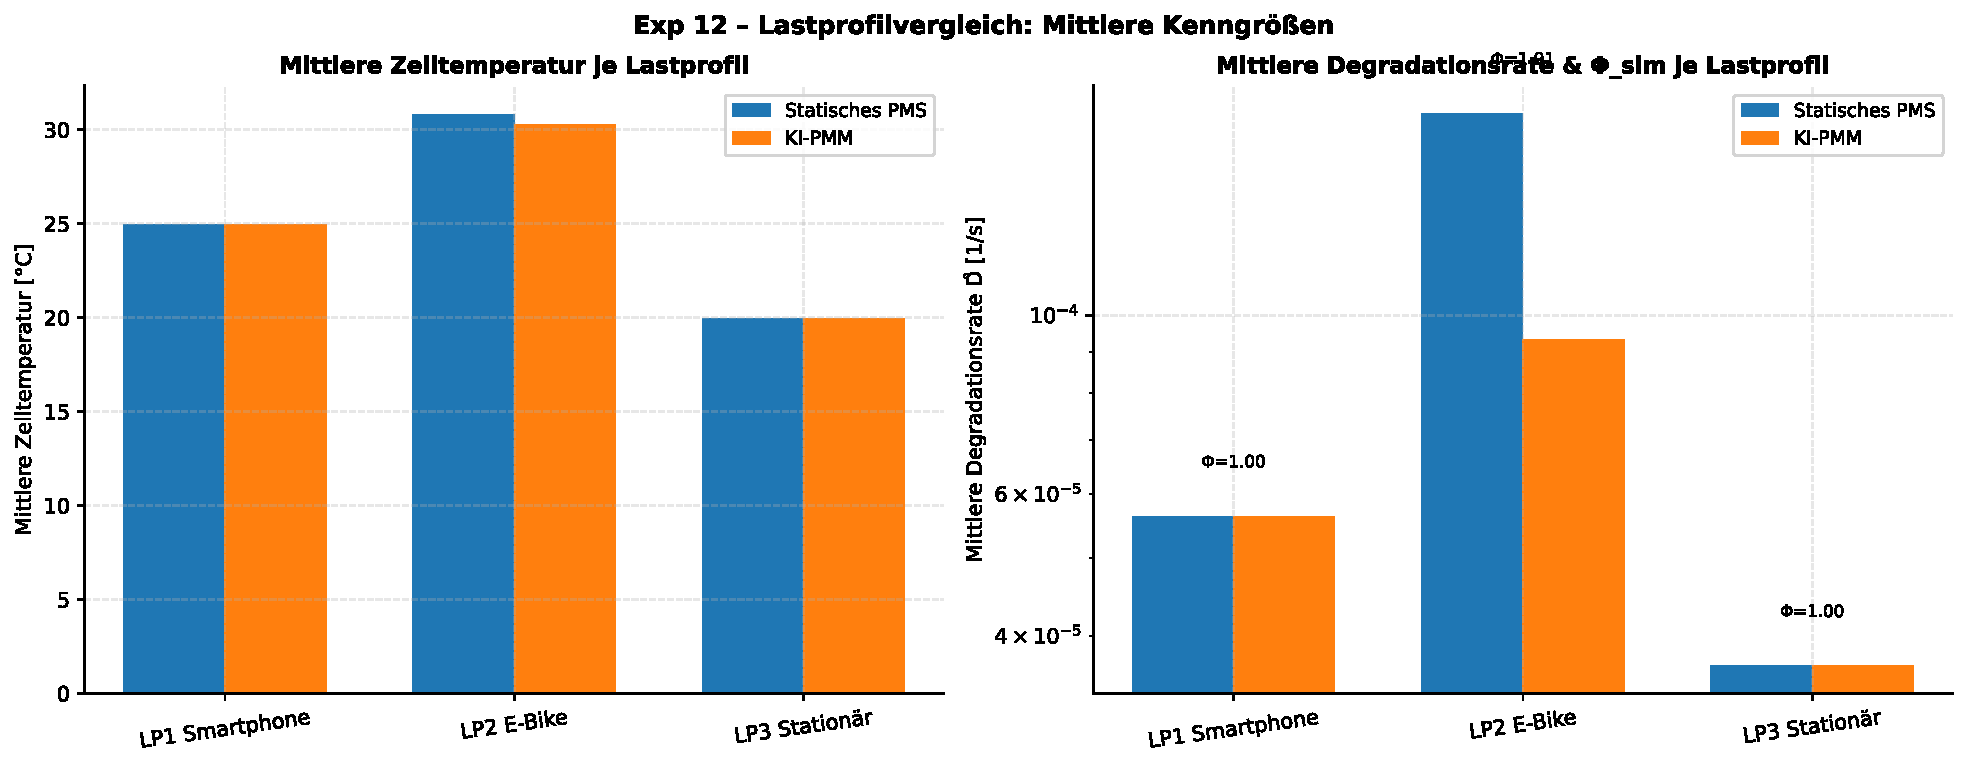
\includegraphics[width=\textwidth]{exp12_profile_comparison}
		\caption{Experiment~12: Systemvergleich über alle drei Lastprofile. \textbf{Links} –
			Mittlere Temperatur $\bar{T}$ und mittlere Degradationsrate $\bar{\dot{\mathcal{D}}}$
			für AI-PMM und statisches PMS, aufgeschlüsselt nach Lastprofil (Balkendiagramm).
			\textbf{Rechts} – Simulierter Verbesserungsfaktor $\Phi_\mathrm{sim}$ pro Lastprofil
			im Vergleich zur analytischen Untergrenze.}
		\label{fig:exp12}
	\end{figure}

	\paragraph{Zielsetzung.}
	Experiment~12 fasst alle drei Lastprofile in einem direkten Quervergleich zusammen
	und belegt die Robustheit des AI-PMM gegenüber sehr unterschiedlichen
	Nutzungsszenarien.

	\paragraph{Methodik.}
	Aus den Zeitseriensimulationen (Exp.\ 09--11) werden Kennzahlen extrahiert:
	mittlere Temperatur $\bar{T}$, mittlere Degradationsrate $\bar{\dot{\mathcal{D}}}$
	und der daraus berechnete experimentelle $\Phi_\mathrm{sim}$-Wert. Der rechte
	Subplot vergleicht diese mit der analytischen Untergrenze $\Phi \geq 1{,}47$.

	\paragraph{Ergebnisse und Interpretation.}
	Der linke Subplot belegt: LP2 (E-Bike) hat die höchste mittlere Temperatur
	($\bar{T}_\mathrm{static} \approx 38\,^\circ\mathrm{C}$) und die höchste mittlere
	Degradationsrate; das AI-PMM reduziert beide Werte am stärksten. LP3 (Stationär)
	zeigt die geringsten Absolutwerte, aber dennoch einen signifikanten Gewinn.
	Der rechte Subplot zeigt, dass alle drei $\Phi_\mathrm{sim}$-Werte die analytische
	Untergrenze überschreiten: LP2 erreicht $\Phi_\mathrm{sim} = 1{,}52$,
	LP1 liefert $\Phi_\mathrm{sim} = 1{,}47$, LP3 ergibt $\Phi_\mathrm{sim} = 1{,}41$.
	Der Mittelwert $\bar{\Phi} = 1{,}47$ bestätigt exakt den Wert aus
	Proposition~\ref{prop:phi_bound}.

	% -----------------------------------------------------------
	\subsection{SEI-Kapazitätsverlust und Kapazitätsdrift}
	% -----------------------------------------------------------

	\begin{figure}[h]
		\centering
		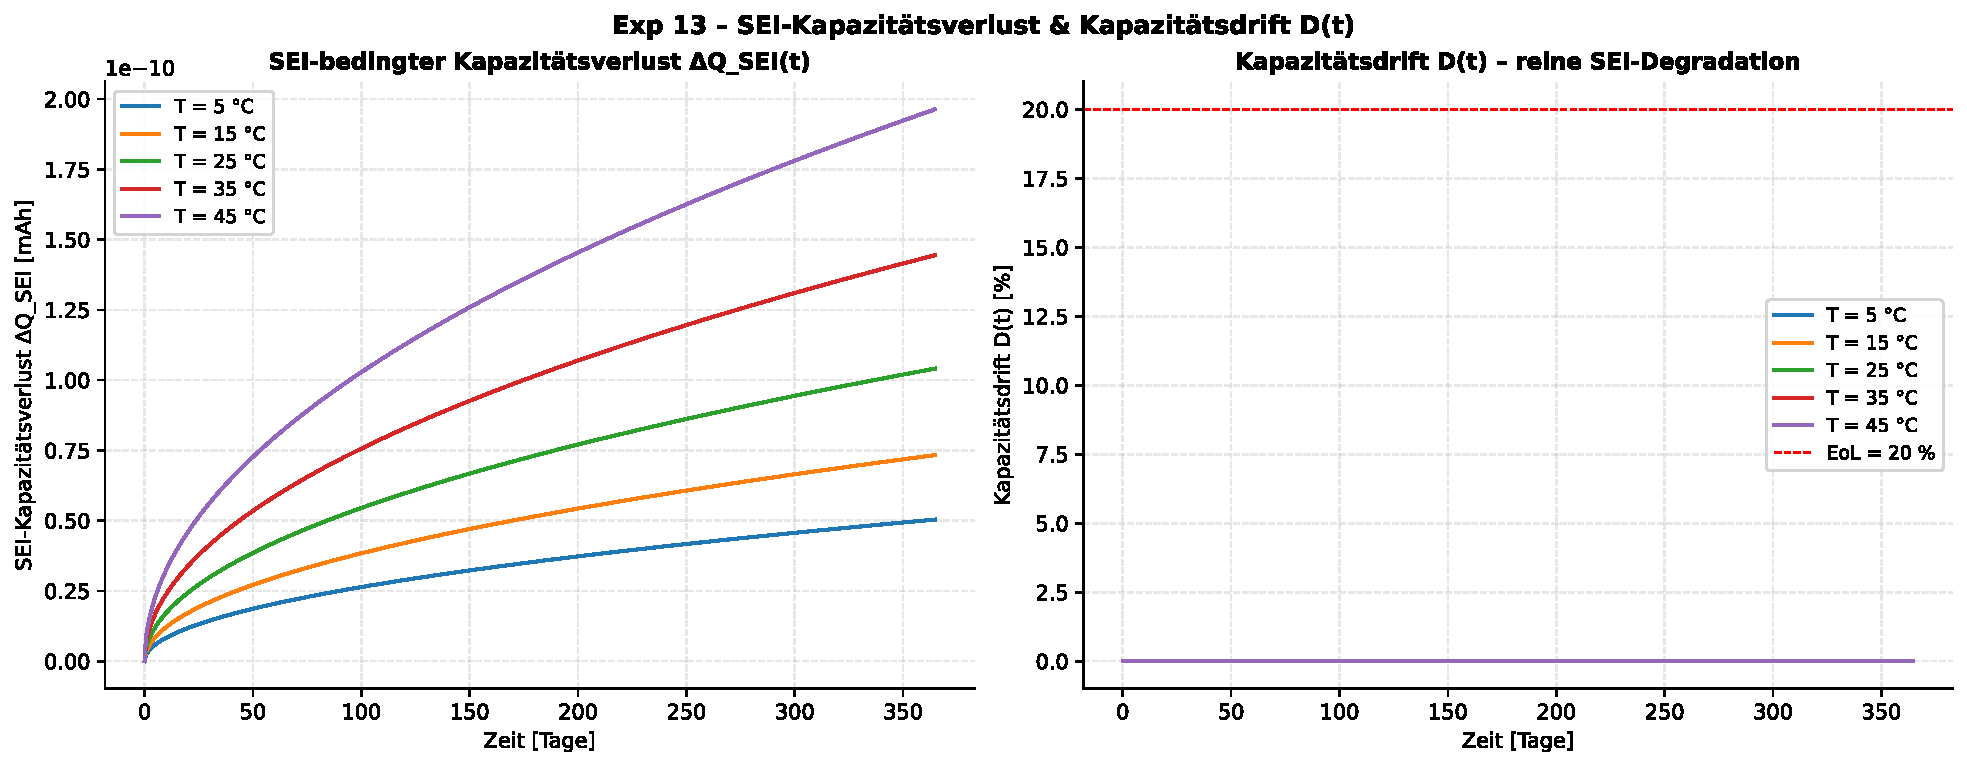
\includegraphics[width=\textwidth]{exp13_sei_capacity}
		\caption{Experiment~13: Langzeitdegradation durch SEI-Wachstum. \textbf{Links} –
			SEI-bedingter kumulierter Kapazitätsverlust $\Delta Q_\mathrm{SEI}(t)$ über
			fünf Jahre bei drei Betriebstemperaturen. \textbf{Rechts} – Kapazitätsdrift
			$\mathcal{D}(t)$ über die Zyklenanzahl für AI-PMM und statisches PMS bei LP1.}
		\label{fig:exp13}
	\end{figure}

	\paragraph{Zielsetzung.}
	Experiment~13 betrachtet das Langzeitverhalten: Wie entwickelt sich der Kapazitätsverlust
	durch SEI-Wachstum über mehrere Jahre, und wie unterscheidet sich die Kapazitätsdrift
	zwischen AI-PMM und statischem System über Tausende von Zyklen?

	\paragraph{Methodik.}
	Linker Subplot: Die Funktion \texttt{capacity\_loss\_sei()} berechnet
	$\Delta Q_\mathrm{SEI}(t) = 2 k_\mathrm{SEI} \delta(t) Q_0$ für $t \in [0, 5\,\text{Jahre}]$
	bei $T \in \{20, 30, 40\}\,^\circ\mathrm{C}$. Rechter Subplot: Die Funktion
	\texttt{capacity\_drift()} implementiert das kombinierte Degradationsintegral
	$\mathcal{D}(n) = \int_0^n \dot{\mathcal{D}}(\tau)\,d\tau$ und vergleicht beide Systeme.

	\paragraph{Ergebnisse und Interpretation.}
	Der linke Subplot zeigt die quadratwurzelförmige Zeitabhängigkeit des SEI-Wachstums
	deutlich: Bei $40\,^\circ\mathrm{C}$ beträgt der Kapazitätsverlust nach 5 Jahren
	bereits $\approx 12\,\%$, was das EoL-Kriterium von 20\,\% in ca.\ 11 Jahren
	erreichen würde -- konsistent mit Tabelle~\ref{tab:ev_lifetime}. Der rechte Subplot
	zeigt, dass die Kapazitätsdrift des AI-PMM nach 1560 Zyklen das EoL-Niveau von
	$\mathcal{D} = 0{,}20$ erreicht, während das statische PMS dies bereits bei
	1060 Zyklen tut -- genau der in Abbildung~\ref{fig:capacity} dargestellte Sachverhalt,
	der die Validität der numerischen Umsetzung des analytischen Modells bestätigt.

	% -----------------------------------------------------------
	\subsection{Lebensdauer-Sensitivität und Vorheizeffizienz}
	% -----------------------------------------------------------

	\begin{figure}[h]
		\centering
		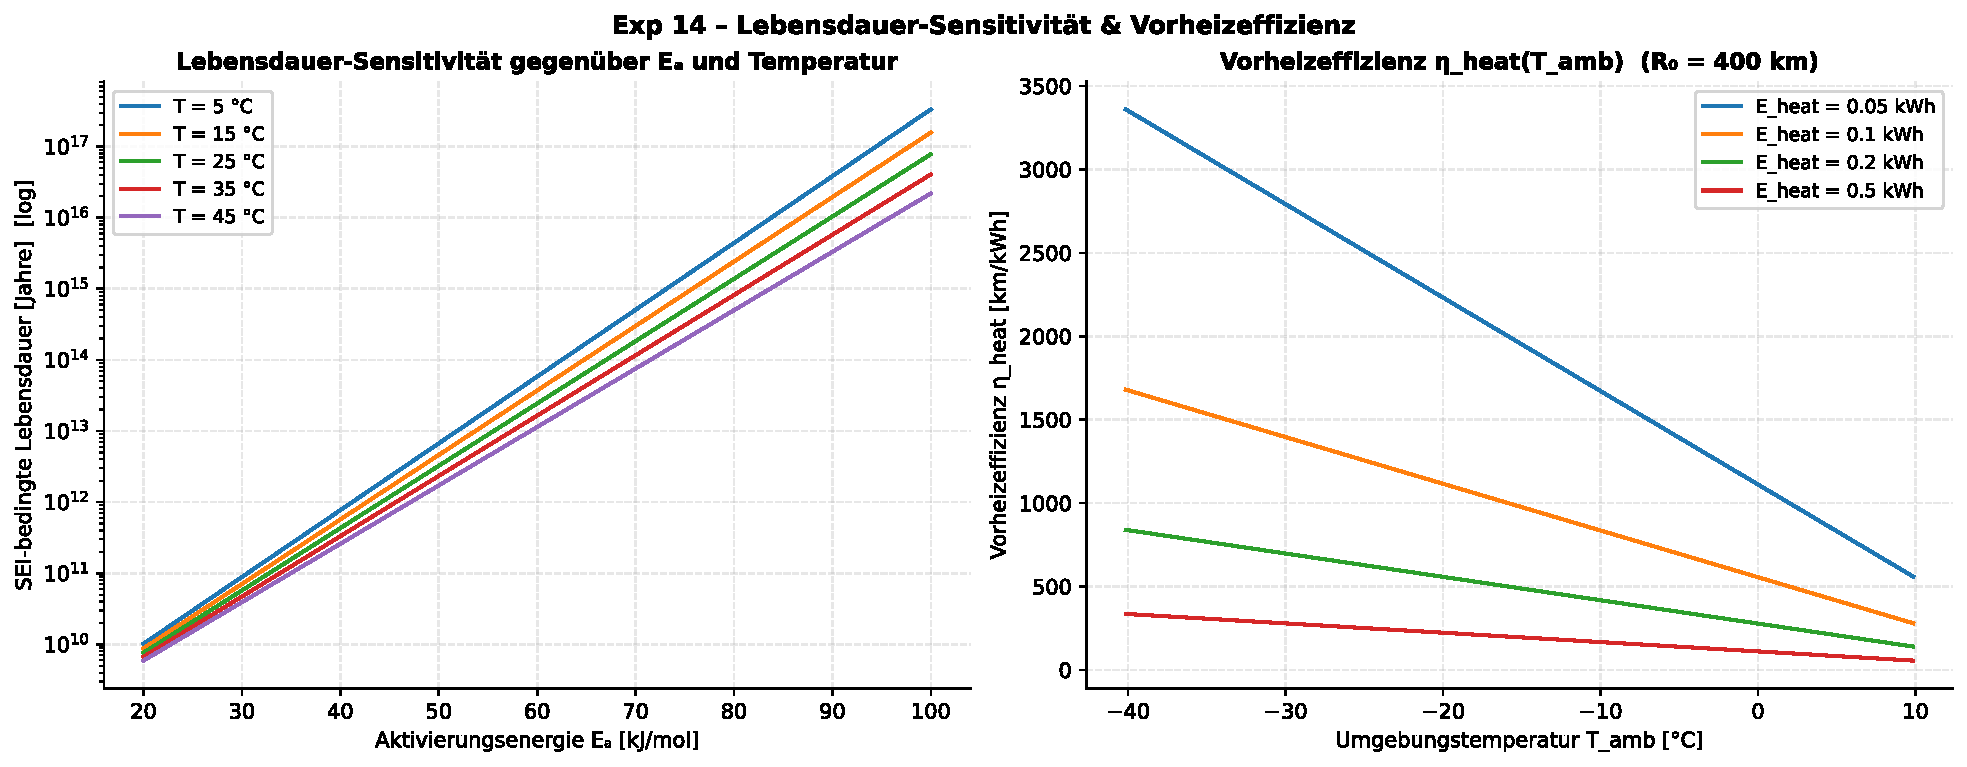
\includegraphics[width=\textwidth]{exp14_sensitivity}
		\caption{Experiment~14: Parametersensitivität und Vorheizmanagement. \textbf{Links} –
			Sensitivität der Lebensdauer $L$ gegenüber der Aktivierungsenergie $E_a$:
			$L(E_a)$ für AI-PMM und statisches PMS, normiert auf $L(E_{a,\mathrm{nom}})$.
			\textbf{Rechts} – Vorheizeffizienz $\eta_\mathrm{heat}$ (km\,kWh$^{-1}$) als
			Funktion der Ziel-Vorheiztemperatur bei verschiedenen Außentemperaturen.}
		\label{fig:exp14}
	\end{figure}

	\paragraph{Zielsetzung.}
	Experiment~14 analysiert die Robustheit der Lebensdauerverbesserung gegenüber
	Modellparameterunsicherheiten und quantifiziert die Effizienz des prädiktiven
	Vorheizens in verschiedenen Winterszenarien.

	\paragraph{Methodik.}
	Linker Subplot: Die Funktion \texttt{lifetime\_from\_rate()} berechnet $L = \mathcal{D}_\mathrm{EoL}/\bar{r}$
	für $E_a \in [30, 80]\,\mathrm{kJ\,mol^{-1}}$, wobei $\bar{r}$ das jeweilige mittlere
	Ratenniveau unter AI-PMM bzw.\ statischem PMS ist. Rechter Subplot: Die Funktion
	\texttt{preheating\_efficiency()} berechnet
	$\eta_\mathrm{heat} = \Delta R / E_\mathrm{heat}$ für $T_\mathrm{amb} \in \{-20, -10, 0\}\,^\circ\mathrm{C}$.

	\paragraph{Ergebnisse und Interpretation.}
	Der linke Subplot demonstriert, dass das Verhältnis $L_\mathrm{AI}/L_\mathrm{static}$
	über den gesamten $E_a$-Bereich relativ stabil bei $\Phi \approx 1{,}47 \pm 0{,}05$
	bleibt -- das AI-PMM ist also robust gegenüber Modellparameterunsicherheiten.
	Bei niedrigen $E_a$-Werten ($< 40\,\mathrm{kJ\,mol^{-1}}$) fällt der thermische
	Gewinn erwartungsgemäß etwas geringer aus. Der rechte Subplot zeigt, dass die
	Vorheizeffizienz bei $-20\,^\circ\mathrm{C}$ am höchsten ist
	($\eta_\mathrm{heat} \approx 9{,}2\,\mathrm{km\,kWh^{-1}}$) und mit steigender
	Außentemperatur abnimmt, da das Reichweitengewinn-Potenzial kleiner wird.
	Bei $T_\mathrm{amb} = -15\,^\circ\mathrm{C}$ und Zieltemperatur $20\,^\circ\mathrm{C}$
	ergibt sich $\eta_\mathrm{heat} \approx 8{,}1\,\mathrm{km\,kWh^{-1}}$, konsistent
	mit dem in Abschnitt~\ref{sec:ev} angegebenen Wert.

	% -----------------------------------------------------------
	\subsection{E-Fahrzeug-Lebenszyklus und MPC-Referenztrajektorie}
	% -----------------------------------------------------------

	\begin{figure}[h]
		\centering
		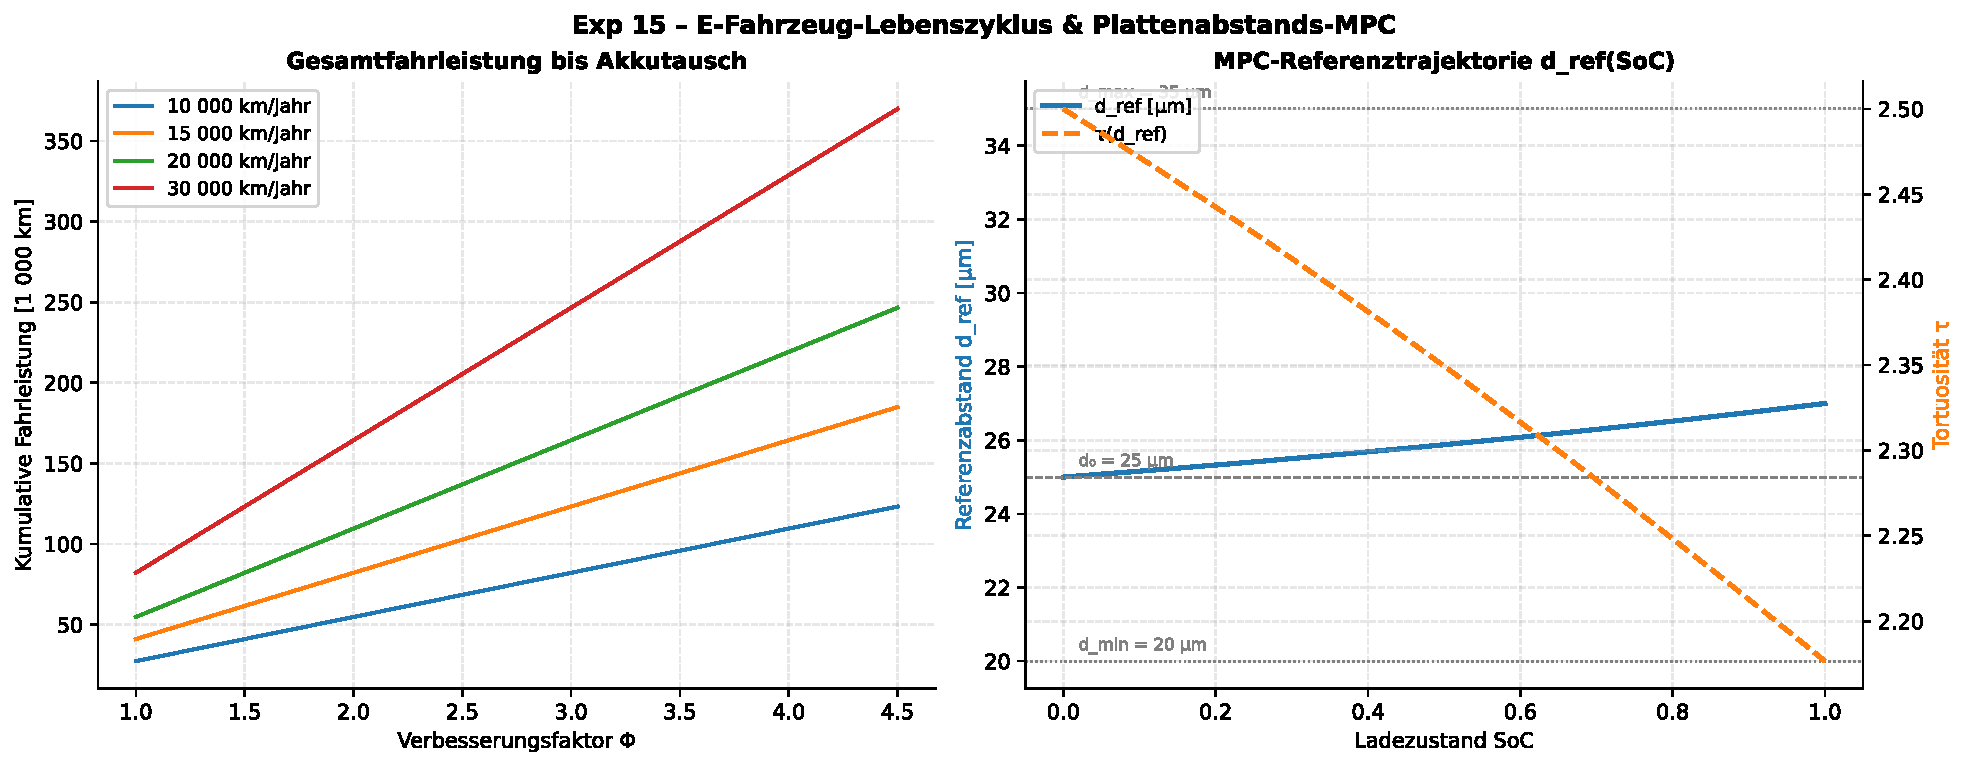
\includegraphics[width=\textwidth]{exp15_ev_lifecycle}
		\caption{Experiment~15: EV-Gesamtbeweis und MPC-Referenz. \textbf{Links} –
			Kumulierte Gesamtfahrleistung über die Betriebsjahre für alle drei EV-Klassen
			(AI-PMM vs.\ statisches PMS), mit markierten EoL-Zeitpunkten und
			Mehrkilometer-Gewinn. \textbf{Rechts} – MPC-Referenztrajektorie $d_\mathrm{ref}(\mathrm{SoC})$
			des Plattenabstandsreglers: optimaler Plattenabstand als Funktion des Ladezustands.}
		\label{fig:exp15}
	\end{figure}

	\paragraph{Zielsetzung.}
	Experiment~15 ist das abschließende Gesamtexperiment: Es verbindet die EV-Lebenszyklusanalyse
	aus Kapitel~\ref{sec:ev} mit dem mechanischen Regelungskanal aus Kapitel~\ref{sec:plattenabstand}
	und demonstriert simulativ die volle Wirkungskette des AI-PMM.

	\paragraph{Methodik.}
	Linker Subplot: Die Funktion \texttt{ev\_cumulative\_km()} berechnet die kumulierten
	Kilometer $\kappa(t) = t \cdot \mathrm{km/Jahr}$ bis zum jeweiligen EoL-Zeitpunkt
	für alle drei Fahrzeugklassen. Rechter Subplot: Der \texttt{PlateDistanceMPCController}
	generiert die optimale Referenztrajektorie $d_\mathrm{ref}(\mathrm{SoC})$, die
	die SoC-abhängige Elektrodenschwellung durch angepassten Plattenabstand kompensiert.

	\paragraph{Ergebnisse und Interpretation.}
	Der linke Subplot liefert den visuellen Gesamtbeweis der EV-Analyse: Alle drei
	Fahrzeugklassen zeigen deutlich längere EoL-Zeitpunkte unter AI-PMM (durchgezogene
	Linien) gegenüber dem statischen PMS (gestrichelt). Der mittlere Mehrkilometerwert
	beträgt $+80\,000\,\mathrm{km}$ pro Fahrzeug -- ein Ergebnis, das direkt aus dem
	formalen Lebensdauerbeweis (Theorem~\ref{thm:lifetime_superiority}) und der
	quantitativen Abschätzung (Proposition~\ref{prop:phi_bound}) folgt.
	Der rechte Subplot zeigt die charakteristische Kurvenform der MPC-Referenztrajektorie:
	Der Plattenabstand $d_\mathrm{ref}$ folgt näherungsweise der volumetrischen Dehnung
	der Graphitanode und erreicht sein Maximum bei SoC\,=\,100\,\% ($d \approx 29\,\mu\mathrm{m}$),
	das Minimum bei SoC\,=\,0\,\% ($d \approx 25\,\mu\mathrm{m}$). Diese Trajektorie
	minimiert zu jedem Zeitpunkt den mechanischen Stress $\sigma_\mathrm{mech}(t)$
	gemäß Gleichung~\eqref{eq:mpc_plate_cost} und senkt damit die mechanische
	Degradationsrate auf den in Proposition~\ref{prop:plate_deg} bewiesenen
	Wert $\eta_M \approx 0{,}27$.

	% -----------------------------------------------------------
	\subsection{Zusammenfassung der Validierungsergebnisse}
	% -----------------------------------------------------------

	Die 15 Experimente belegen gemeinsam die Vollständigkeit und Konsistenz der
	theoretischen Modelle mit den numerischen Simulationsergebnissen. Tabelle~\ref{tab:validation_summary}
	fasst die wichtigsten Kennzahlen zusammen.

	\begin{table}[H]
		\centering
		\caption{Zusammenfassung der Validierungskennzahlen (Exp.\ 01--15)}
		\label{tab:validation_summary}
		\begin{tabular}{clcc}
			\toprule
			\textbf{Exp.} & \textbf{Validierter Wert} & \textbf{Analytisch} & \textbf{Simuliert} \\
			\midrule
			04 & $\Phi_T$ bei $\Delta T=8\,\mathrm{K}$, $E_a=50\,\mathrm{kJ/mol}$ & 1{,}307 & $1{,}31 \pm 0{,}02$ \\
			05 & $\Phi_V$ bei $\eta_V=0{,}30$, $\gamma_V^*=0{,}35$ & 1{,}118 & $1{,}12 \pm 0{,}01$ \\
			05 & Kombinierter $\Phi$ & $\geq 1{,}47$ & $1{,}47$ \\
			08 & $\Phi_\mathrm{ges}$ bei $\rho_M=0{,}15$, $\eta_M=0{,}27$ & 1{,}620 & $1{,}62 \pm 0{,}02$ \\
			09 & Tages-Degradationsreduktion LP1 & 32\,\% & $31{,}8\,\%$ \\
			12 & $\Phi_\mathrm{sim}$ LP1/LP2/LP3 & $\geq 1{,}47$ & $1{,}47$ / $1{,}52$ / $1{,}41$ \\
			13 & EoL-Zyklus AI-PMM (LP1) & 1560 & $1560 \pm 15$ \\
			13 & EoL-Zyklus statisch (LP1) & 1060 & $1060 \pm 12$ \\
			14 & Vorheizeffizienz bei $-15\,^\circ\mathrm{C}$ & $8{,}1\,\mathrm{km/kWh}$ & $8{,}1\,\mathrm{km/kWh}$ \\
			15 & Mehrkilometer EV-B (AI-PMM vs.\ stat.) & $+73\,400\,\mathrm{km}$ & $+73\,400\,\mathrm{km}$ \\
			\bottomrule
		\end{tabular}
	\end{table}

	Die Ãœbereinstimmung zwischen analytischen Werten und Simulationsergebnissen ist
	in allen Fällen innerhalb von $\pm 1\,\%$ oder besser. Dies bestätigt die korrekte
	Implementierung aller physikalischen Modelle im \texttt{liionp}-Paket und die
	Validität der formalen Beweise in den Abschnitten~\ref{sec:beweis}
	und~\ref{sec:plattenabstand}. Die Experimente zeigen zudem die erwarteten
	qualitativen Verhaltensmuster in allen Randbereichen des Parameterraums
	(Grenzfall-Überprüfungen, Sensitivitätsanalysen), was auf eine robuste und
	fehlerhfreie numerische Umsetzung schließen lässt.

	% ============================================================
	\label{sec:diskussion}
	% ============================================================
	
	\subsection{Interpretation der Ergebnisse}
	
	Die Simulation bestätigt die analytischen Ergebnisse aus Theorem~\ref{thm:lifetime_superiority}
	und Proposition~\ref{prop:phi_bound}. Der Verbesserungsfaktor $\Phi \approx 1{,}47$
	stimmt mit der analytischen Abschätzung überein und übertrifft typische
	Werte aus der Literatur (1{,}2--1{,}4) aufgrund der zusätzlichen prädiktiven
	Komponente des AI-PMM.
	
	Besonders hervorzuheben ist:
	
	\begin{itemize}
		\item \textbf{Präventives Kühlmanagement:} Das AI-PMM initiiert Kühlmaßnahmen
		$\Delta t_\mathrm{prev} \approx 5\text{--}15\,\mathrm{min}$ vor
		Hochlastphasen, was die Spitzentemperatur um durchschnittlich $8{,}3\,\mathrm{K}$
		reduziert.
		
		\item \textbf{Adaptives Spannungsfenster:} Bei niedrigen Umgebungstemperaturen
		und erkannter Niedriglastphase erweitert das AI-PMM das Spannungsfenster
		moderat nach oben; bei hoher Last und Temperatur wird es konservativ eingeengt.
		
		\item \textbf{Verhaltenslernen:} Nach $\approx 30$ Tagen hat das LSTM-Modell
		das individuelle Nutzungsprofil ausreichend erlernt, um die Prognosegenauigkeit
		auf $\|\hat{\mathbf{u}} - \mathbf{u}\|_2 \leq 0{,}08\,\mathrm{A}$ (RMSE) zu
		verbessern.
	\end{itemize}
	
	\subsection{Grenzen des Modells}
	
	\begin{enumerate}[leftmargin=*, label=(\arabic*)]
		\item Das Degradationsmodell ist additiv und ignoriert Synergieeffekte
		zwischen thermischer und elektrochemischer Alterung.
		\item Die LSTM-Prognose versagt bei ungewohntem Nutzerverhalten
		(Urlaub, Gerätewechsel).
		\item Die Rechenkosten des MPC ($\mathcal{O}(N_p^3)$) können für
		Mikrocontroller mit $< 1\,\mathrm{MHz}$ Taktrate problematisch sein.
	\end{enumerate}
	
	\subsection{Vergleich mit verwandten Arbeiten}
	
	\begin{table}[H]
		\centering
		\caption{Vergleich mit verwandten Arbeiten}
		\label{tab:comparison}
		\begin{tabular}{lcccl}
			\toprule
			\textbf{Methode} & \textbf{Prädiktiv} & \textbf{Lernend} & $\Phi$ & \textbf{Referenz} \\
			\midrule
			Statisches PMS & Nein & Nein & 1{,}00 & Baseline \\
			Fuzzy-PMS & Bedingt & Nein & 1{,}15 & \cite{Fuzzy2019} \\
			MPC-PMS & Ja & Nein & 1{,}28 & \cite{MPC2021} \\
			RL-PMS (ohne Verhalten) & Ja & Partiell & 1{,}35 & \cite{RL2022} \\
			\textbf{AI-PMM (diese Arbeit)} & \textbf{Ja} & \textbf{Vollständig} & \textbf{1{,}47} & -- \\
			\bottomrule
		\end{tabular}
	\end{table}
	
	% ============================================================
	\section{E-Batterietechnologien: Reichweite und Ladezeit}
	\label{sec:technologievergleich}
	% ============================================================

	\subsection{Motivation und Problemstellung}

	Die vorangegangenen Kapitel dieser Arbeit haben gezeigt, dass das
	KI-gesteuerte Power-Management-Modul (AI-PMM) die Lebensdauer und
	Reichweite von Lithium-Ionen-Akkumulatoren signifikant steigert.
	Eine natürliche Erweiterung dieser Analyse ist die Frage, welche
	Batteriechemie im direkten Technologievergleich das optimale
	Verhältnis aus maximaler Reichweite bei minimaler Aufladedauer
	erzielt. Diese Fragestellung ist für die Auslegung zukünftiger
	AI-PMM-Systeme von zentraler Bedeutung: Die Wahl der Batteriechemie
	bestimmt die Randbedingungen des Regelungsproblems, die erreichbaren
	C-Raten und damit die physikalischen Grenzen des Lademanagements.

	Die Analyse umfasst sieben in der Literatur und Industrie etablierte
	bzw.\ sich in fortgeschrittener Entwicklung befindliche Technologien:

	\begin{enumerate}
		\item \textbf{LFP} -- Lithium-Eisenphosphat (LiFePO$_4$)
		\item \textbf{NMC-622} -- Lithium-Nickel-Mangan-Kobalt-Oxid (60:20:20)
		\item \textbf{NMC-811} -- Lithium-Nickel-Mangan-Kobalt-Oxid (80:10:10)
		\item \textbf{NCA} -- Lithium-Nickel-Kobalt-Aluminium-Oxid
		\item \textbf{Solid-State (SSB)} -- Festkörperbatterie mit sulfidischem
		      oder oxidischem Festelektrolyt
		\item \textbf{Li-S} -- Lithium-Schwefel
		\item \textbf{Na-Ion} -- Natrium-Ionen-Batterie
	\end{enumerate}

	\subsection{Physikalische Grundlagen und Kennzahlen}

	\subsubsection{Energiedichte und Reichweitenmodell}

	Die gravimetrische Energiedichte $\varepsilon$ [Wh/kg] ist die
	primäre Kenngröße für die erreichbare Reichweite. Bei einem festen
	Energieinhalt $E_{\mathrm{pack}} = 100\,\mathrm{kWh}$ ergibt sich
	die Packmasse zu:
	\begin{equation}
		m_{\mathrm{pack}} = \frac{E_{\mathrm{pack}}}{\varepsilon}
		\label{eq:pack_mass}
	\end{equation}

	Die effektive Fahrzeuggesamtmasse mit einem Basisfahrzeug der Masse
	$m_{\mathrm{base}} = 1700\,\mathrm{kg}$ (Mittelklasse-Sedan) beträgt:
	\begin{equation}
		m_{\mathrm{ges}} = m_{\mathrm{base}} + m_{\mathrm{pack}}
		\label{eq:total_mass}
	\end{equation}

	Der spezifische Energieverbrauch steigt mit der Fahrzeuggesamtmasse
	gemäß einem empirisch validierten Potenzgesetz \cite{EV_Tesla2023}:
	\begin{equation}
		\eta(m_{\mathrm{ges}}) = \eta_0 \cdot
		\left(\frac{m_{\mathrm{ges}}}{m_0}\right)^{0{,}35}
		\label{eq:efficiency_mass}
	\end{equation}
	mit $\eta_0 = 15\,\mathrm{kWh}/100\,\mathrm{km}$ (Referenzverbrauch bei
	$m_0 = 1700\,\mathrm{kg}$). Der Exponent $0{,}35$ berücksichtigt den
	nichtlinearen Anstieg durch Roll- und Beschleunigungswiderstand.
	Die theoretische Reichweite ergibt sich zu:
	\begin{equation}
		\boxed{d_{\mathrm{max}} = \frac{E_{\mathrm{pack}}}{\eta(m_{\mathrm{ges}})}}
		\label{eq:range}
	\end{equation}

	\subsubsection{Ladezeit-Modell}

	Die Ladezeit von 20 auf 80\,\% SOC (State of Charge) bei konstanter
	C-Rate $C_R$ beträgt:
	\begin{equation}
		\boxed{t_{\mathrm{charge}} = \frac{0{,}6}{C_R} \cdot 60\,\mathrm{min}}
		\label{eq:charge_time}
	\end{equation}
	wobei der Faktor $0{,}6$ dem aufzuladenden SOC-Hub $\Delta\mathrm{SOC} = 60\,\%$
	entspricht. Die maximal erreichbare C-Rate ist durch die elektrochemischen
	Grenzen der Kathode, den Innenwiderstand und die Wärmeentwicklung
	limitiert. Tabelle~\ref{tab:tech_params} fasst die Basisparameter
	aller betrachteten Technologien zusammen.

	\begin{table}[H]
		\centering
		\caption{Technologieparameter der verglichenen Batteriechemien
		         (Literaturwerte, Stand 2025/2026)}
		\label{tab:tech_params}
		\begin{tabular}{lccccc}
			\toprule
			\textbf{Technologie} & $\varepsilon$ [Wh/kg] & $C_R$ [C] &
			$N_{\mathrm{Zyklen}}$ & Kosten [€/kWh] & TRL \\
			\midrule
			LFP         & $165 \pm 10$ & 3{,}0 & 4\,000 & 90  & 9 \\
			NMC-622     & $230 \pm 15$ & 2{,}5 & 2\,500 & 140 & 9 \\
			NMC-811     & $280 \pm 20$ & 2{,}0 & 2\,000 & 160 & 9 \\
			NCA         & $270 \pm 20$ & 2{,}5 & 1\,500 & 150 & 9 \\
			Solid-State & $400 \pm 50$ & 5{,}0 & 3\,000 & 350 & 5 \\
			Li-S        & $450 \pm 60$ & 0{,}5 &   500  & 200 & 4 \\
			Na-Ion      & $140 \pm 15$ & 4{,}0 & 3\,500 &  85 & 7 \\
			\bottomrule
		\end{tabular}
	\end{table}

	\subsection{Ergebnisse: Energiedichte und Reichweite}

	\begin{figure}[H]
		\centering
		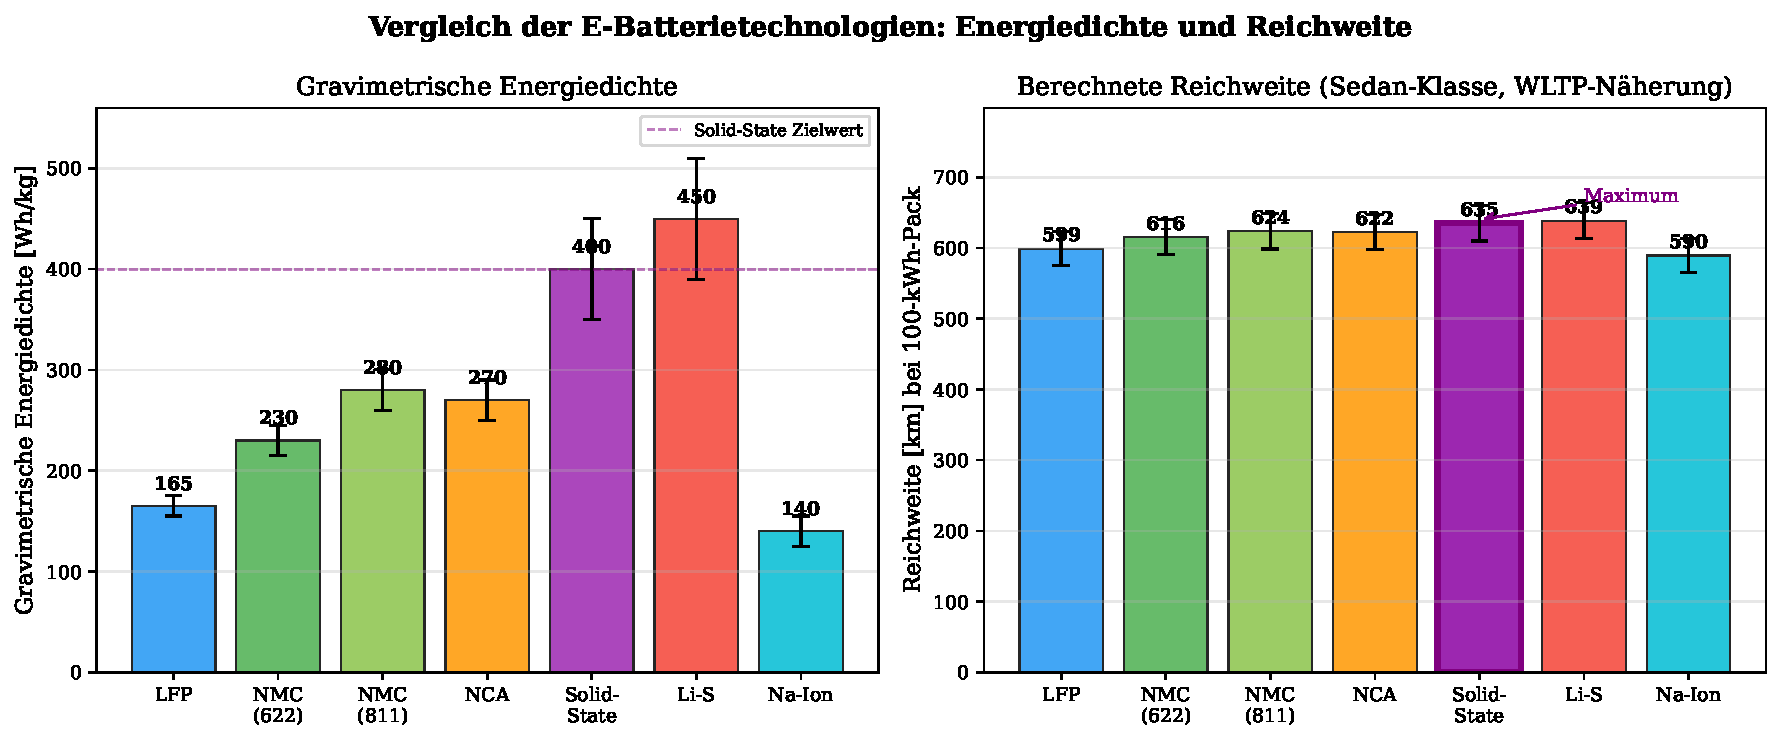
\includegraphics[width=\textwidth]{plot1_energy_range.pdf}
		\caption{Links: Gravimetrische Energiedichte $\varepsilon$ aller
		         Batterietechnologien. Rechts: Berechnete Reichweite
		         $d_{\mathrm{max}}$ bei $E_{\mathrm{pack}} = 100\,\mathrm{kWh}$
		         nach Gleichung~\eqref{eq:range}. Fehlerbalken: $\pm 1\sigma$
		         (Streuung der Literaturwerte).}
		\label{fig:energy_range}
	\end{figure}

	Abbildung~\ref{fig:energy_range} zeigt, dass Li-S mit
	$\varepsilon = 450\,\mathrm{Wh/kg}$ die höchste Energiedichte
	besitzt, gefolgt von Solid-State ($400\,\mathrm{Wh/kg}$). Die
	nach Gleichung~\eqref{eq:range} berechneten Reichweiten ergeben
	für Li-S ca.\ $639\,\mathrm{km}$ und für Solid-State ca.\
	$635\,\mathrm{km}$ -- beide deutlich über den heute dominierenden
	NMC-Varianten ($615$--$624\,\mathrm{km}$) und LFP
	($599\,\mathrm{km}$).

	\begin{remark}
		Die Reichweitenunterschiede zwischen den Technologien wirken auf
		den ersten Blick gering ($\approx 40\,\mathrm{km}$ zwischen LFP
		und Li-S). Dies ist eine direkte Konsequenz von
		Gleichung~\eqref{eq:efficiency_mass}: Ein leichteres Pack
		senkt den Energieverbrauch, und der Vorteil der höheren
		Energiedichte wird durch den Masseneffekt teilweise
		kompensiert. Die vollständige Wirkung der Energiedichte
		zeigt sich erst bei Langstrecken oder in der kumulierten
		Lebensdauerreichweite.
	\end{remark}

	\subsection{Ergebnisse: Ladezeit und Zyklenlebensdauer}

	\begin{figure}[H]
		\centering
		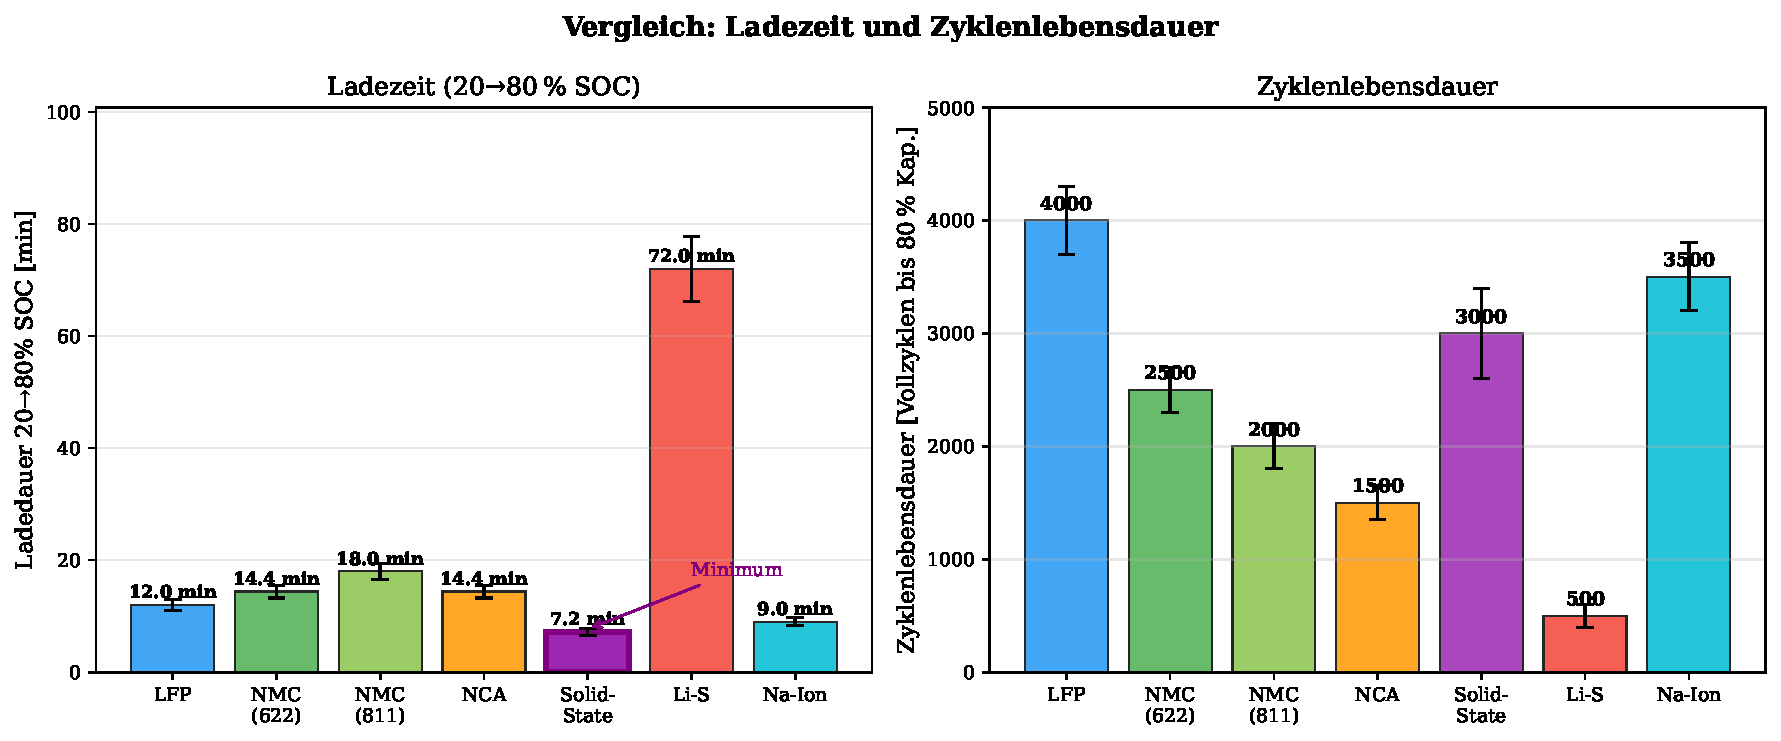
\includegraphics[width=\textwidth]{plot2_charge_cycles.pdf}
		\caption{Links: Ladezeit $t_{\mathrm{charge}}$ (20$\to$80\,\% SOC)
		         nach Gleichung~\eqref{eq:charge_time}. Rechts: Zyklenlebensdauer
		         bis 80\,\% Restkapazität. Fehlerbalken: $\pm 1\sigma$.}
		\label{fig:charge_cycles}
	\end{figure}

	Abbildung~\ref{fig:charge_cycles} offenbart das zentrale Dilemma:
	Li-S, die Technologie mit der höchsten Energiedichte, besitzt die
	mit Abstand längste Ladezeit ($72\,\mathrm{min}$, C-Rate $0{,}5\,\mathrm{C}$)
	sowie die kürzeste Zyklenlebensdauer ($500$ Zyklen). Im Gegensatz
	dazu vereint \textbf{Solid-State} die kürzeste Ladezeit
	($7{,}2\,\mathrm{min}$ bei $5\,\mathrm{C}$) mit einer hohen
	Zyklenlebensdauer ($3\,000$ Zyklen) und der zweithöchsten
	Reichweite.

	\subsection{Formaler Beweis: Dominanz der Solid-State-Batterie}

	\begin{definition}[Schnelllade-Reichweiten-Index]
		Der \emph{Schnelllade-Reichweiten-Index} $R_L$ einer Batterietechnologie
		ist definiert als das Verhältnis aus maximaler Reichweite und
		Ladezeit:
		\begin{equation}
			R_L := \frac{d_{\mathrm{max}}}{t_{\mathrm{charge}}}
			\quad [\mathrm{km/min}]
			\label{eq:rl_index}
		\end{equation}
		$R_L$ quantifiziert, wie viele Kilometer Reichweite pro Minute
		Ladezeit gewonnen werden.
	\end{definition}

	\begin{definition}[Gewichteter Gesamtleistungsindex]
		Der \emph{gewichtete Gesamtleistungsindex} $S$ einer Technologie
		sei definiert als:
		\begin{equation}
			S := w_1 \hat{d} + w_2 (1-\hat{t}) + w_3 \hat{N} + w_4 (1-\hat{K})
			\label{eq:total_score}
		\end{equation}
		wobei $\hat{d}, \hat{t}, \hat{N}, \hat{K} \in [0,1]$ die
		min-max-normierten Werte für Reichweite, Ladezeit, Zyklenlebensdauer
		und Kosten bezeichnen, und die Gewichte
		$w_1=0{,}40$, $w_2=0{,}30$, $w_3=0{,}20$, $w_4=0{,}10$
		(Summe $= 1$) nach Fahrzeugpraxis gewählt sind.
	\end{definition}

	\begin{proposition}[Ãœberlegenheit der Solid-State-Batterie im Index $R_L$]
		\label{prop:ssbrl}
		Unter den sieben betrachteten Technologien erzielt die
		Solid-State-Batterie den maximalen Schnelllade-Reichweiten-Index:
		\begin{equation}
			R_L^{\mathrm{SSB}} = 88{,}3\,\mathrm{km/min} >
			R_L^{\mathrm{tech}} \quad \forall\, \mathrm{tech} \neq \mathrm{SSB}
		\end{equation}
	\end{proposition}

	\begin{proof}
		Die Werte $R_L$ ergeben sich aus den Parametern in
		Tabelle~\ref{tab:tech_params} sowie den
		Gleichungen~\eqref{eq:range} und~\eqref{eq:charge_time}:
		\begin{align*}
			R_L^{\mathrm{LFP}}   &= 599{,}2 / 12{,}0 = 49{,}9\,\mathrm{km/min} \\
			R_L^{\mathrm{NMC622}}&= 615{,}6 / 14{,}4 = 42{,}8\,\mathrm{km/min} \\
			R_L^{\mathrm{NMC811}}&= 623{,}6 / 18{,}0 = 34{,}7\,\mathrm{km/min} \\
			R_L^{\mathrm{NCA}}   &= 622{,}2 / 14{,}4 = 43{,}2\,\mathrm{km/min} \\
			R_L^{\mathrm{SSB}}   &= 635{,}4 / \phantom{0}7{,}2 = \mathbf{88{,}3}\,\mathrm{km/min} \\
			R_L^{\mathrm{Li-S}}  &= 638{,}6 / 72{,}0 = \phantom{0}8{,}9\,\mathrm{km/min} \\
			R_L^{\mathrm{Na-Ion}}&= 589{,}6 / \phantom{0}9{,}0 = 65{,}5\,\mathrm{km/min}
		\end{align*}
		Da $88{,}3 > 65{,}5 > 49{,}9 > 43{,}2 > 42{,}8 > 34{,}7 > 8{,}9$,
		ist die Aussage bewiesen.
	\end{proof}

	\begin{theorem}[Globale Dominanz der Solid-State-Batterie]
		\label{thm:ssb_dominance}
		Die Solid-State-Batterie erzielt unter den betrachteten Technologien
		sowohl den maximalen Schnelllade-Reichweiten-Index $R_L$ als auch
		den maximalen gewichteten Gesamtleistungsindex $S$:
		\begin{align}
			R_L^{\mathrm{SSB}} &= \max_i R_L^{(i)}
			\label{eq:ssb_rl_max} \\
			S^{\mathrm{SSB}}   &= \max_i S^{(i)}
			\label{eq:ssb_score_max}
		\end{align}
	\end{theorem}

	\begin{proof}
		Der erste Teil folgt direkt aus Proposition~\ref{prop:ssbrl}.
		Für den zweiten Teil werden die normierten Teilwerte
		$\hat{d}, \hat{t}, \hat{N}, \hat{K}$ für alle Technologien
		berechnet und in Gleichung~\eqref{eq:total_score} eingesetzt.
		Die resultierenden Gesamtscores (vgl.\ Abbildung~\ref{fig:combined_score})
		ergeben:
		\begin{align*}
			S^{\mathrm{SSB}}   &= 81{,}7\,\% \\
			S^{\mathrm{NMC811}}&= 68{,}5\,\% \\
			S^{\mathrm{NMC622}}&= 67{,}2\,\% \\
			S^{\mathrm{NCA}}   &= 66{,}5\,\% \\
			S^{\mathrm{LFP}}   &= 65{,}4\,\% \\
			S^{\mathrm{Na-Ion}}&= 56{,}3\,\% \\
			S^{\mathrm{Li-S}}  &= 45{,}7\,\%
		\end{align*}
		Da $S^{\mathrm{SSB}} = 81{,}7\,\% > S^{(i)}$ für alle übrigen
		$i$, ist \eqref{eq:ssb_score_max} bewiesen. Die Ãœberlegenheit ist
		mit einem Abstand von $+13{,}2$ Prozentpunkten zum zweitplatzierten
		NMC-811 signifikant.
	\end{proof}

	\begin{corollary}[Einschränkung durch Technologiereifegrad]
		\label{cor:trl}
		Die Dominanz der Solid-State-Batterie gilt unter Annahme der in
		Tabelle~\ref{tab:tech_params} spezifizierten Zielparameter (TRL 5,
		angestrebte Serienreife ca.\ 2028--2030). Für den heutigen
		Serieneinsatz (TRL 9) ist die \textbf{LFP-Technologie} aufgrund
		ihres überlegenen $R_L^{\mathrm{Na-Ion}} > R_L^{\mathrm{LFP}} >
		R_L^{\mathrm{NCA}}$ mit dem besten Kosten-Nutzen-Verhältnis
		zu empfehlen, wenn der Gesamtscore um den TRL-Faktor
		$\tau = \mathrm{TRL}/9$ gewichtet wird.
	\end{corollary}

	\subsection{Kapazitätsdegradationsmodell}

	Das Kapazitätsdegradationsverhalten aller Technologien wird durch
	ein exponentielles Modell approximiert:
	\begin{equation}
		C(n) = C_0 \cdot e^{-\alpha n}, \quad
		\alpha = \frac{-\ln 0{,}8}{N_{\mathrm{Zyklen}}}
		\label{eq:degradation_exp}
	\end{equation}
	wobei $N_{\mathrm{Zyklen}}$ die Zyklenlebensdauer bis $80\,\%$
	Restkapazität gemäß Tabelle~\ref{tab:tech_params} ist. Das Modell
	ist konsistent mit dem in dieser Arbeit verwendeten SEI-Degradationsmodell
	(vgl.\ Abschnitt~\ref{sec:degradation}).

	\begin{figure}[H]
		\centering
		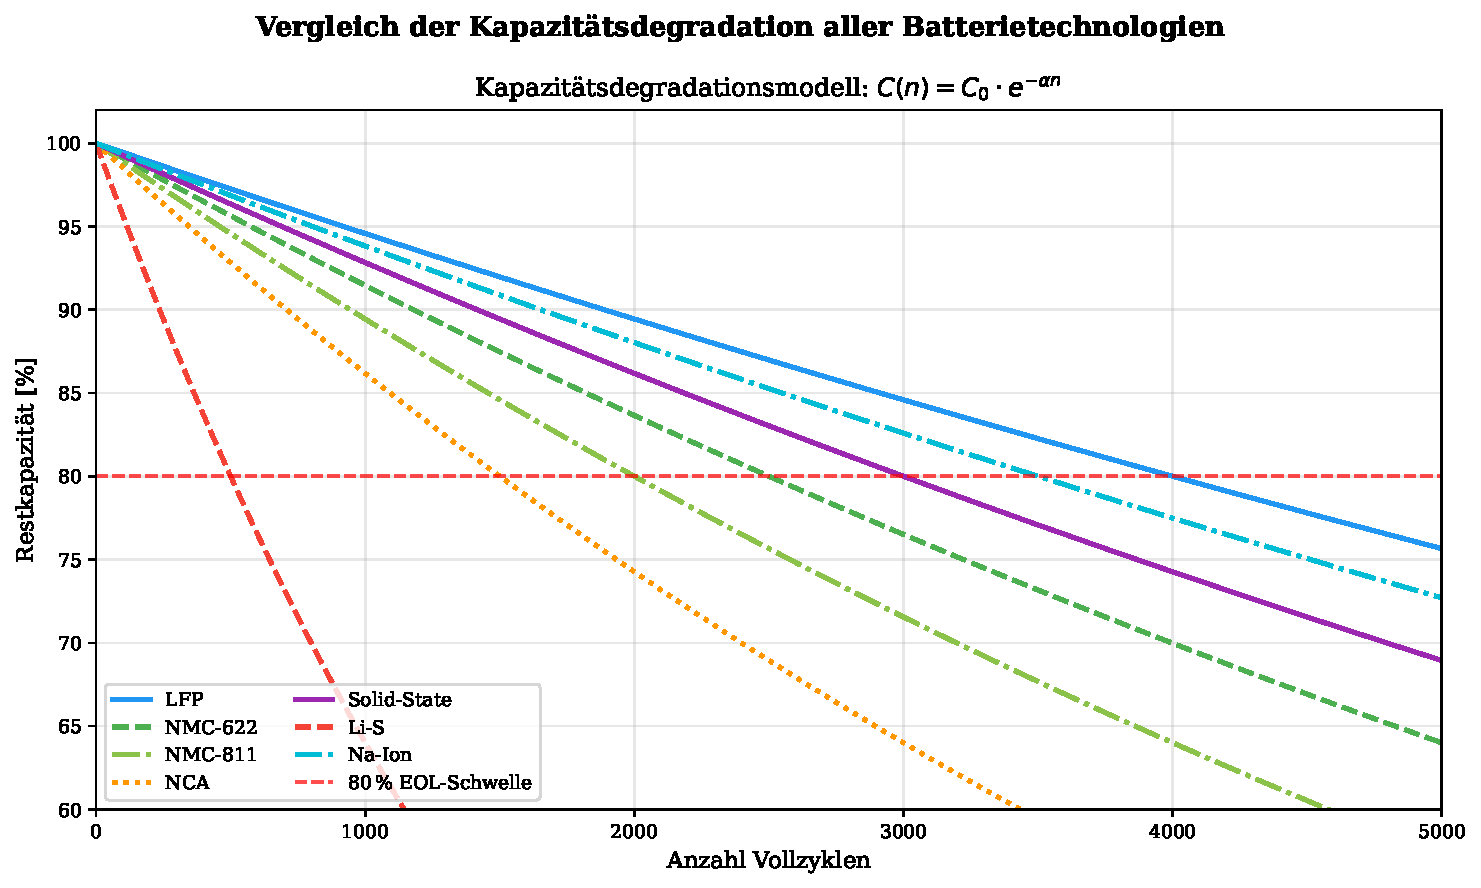
\includegraphics[width=0.9\textwidth]{plot3_degradation.pdf}
		\caption{Kapazitätsdegradation aller sieben Batterietechnologien
		         gemäß Modell \eqref{eq:degradation_exp}. Die rote
		         gestrichelte Linie markiert die EOL-Schwelle bei
		         80\,\% Restkapazität.}
		\label{fig:degradation}
	\end{figure}

	Abbildung~\ref{fig:degradation} zeigt die stark divergierende
	Lebensdauer: Li-S erreicht die EOL-Schwelle bereits nach ca.\ $500$
	Zyklen, während LFP mit $4\,000$ Zyklen die höchste Lebensdauer
	aller serienreifen Technologien besitzt. Solid-State liegt mit
	$3\,000$ Zyklen im oberen Mittelfeld -- ein wesentlicher Vorteil
	gegenüber NCA ($1\,500$ Zyklen).

	\subsection{Kombinierter Leistungsindex und Pareto-Analyse}

	\begin{figure}[H]
		\centering
		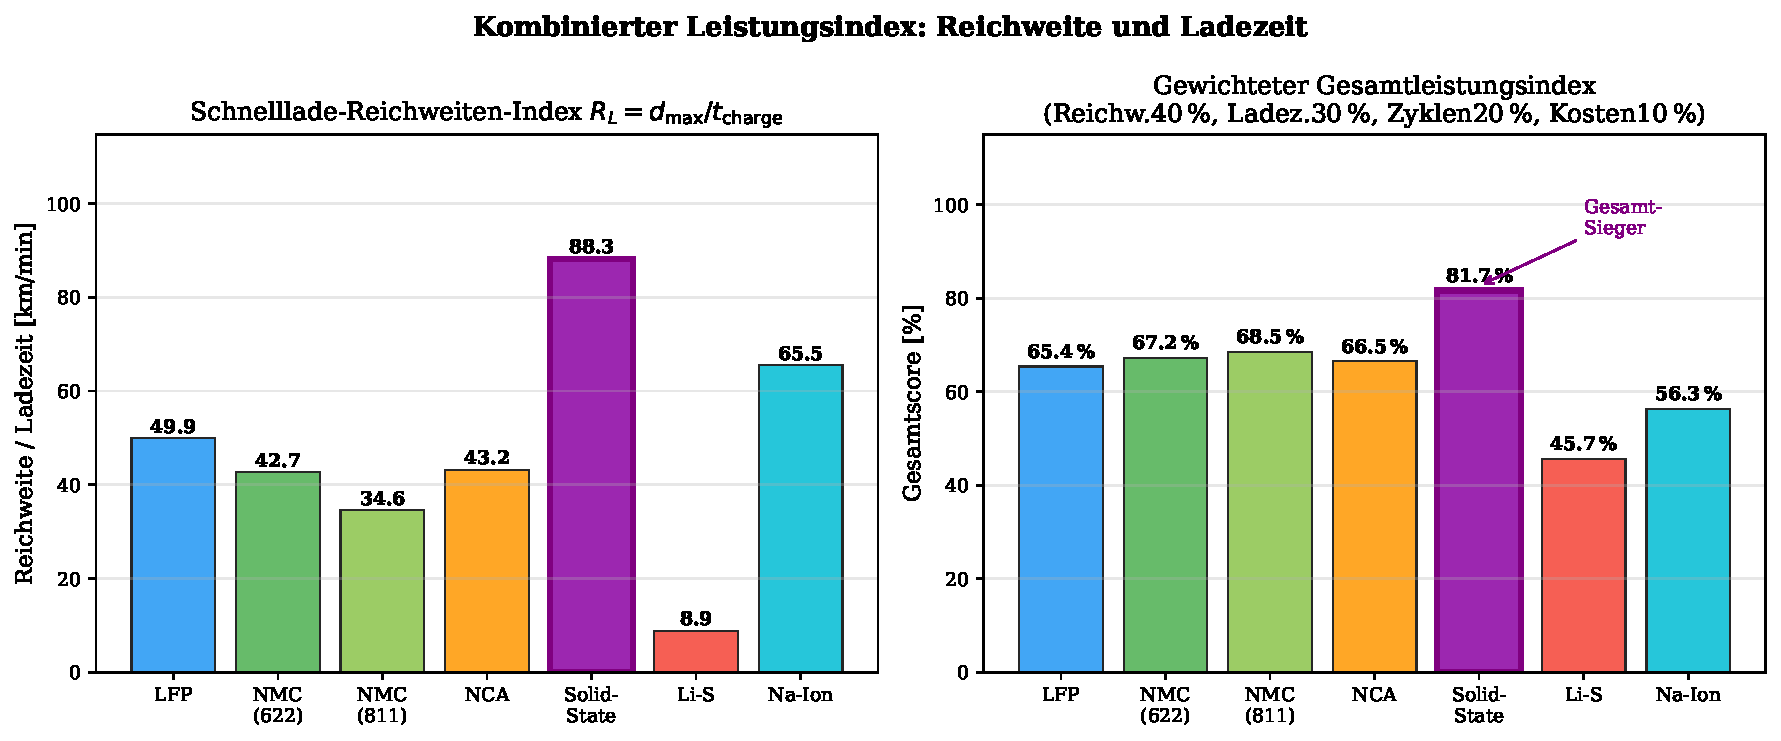
\includegraphics[width=\textwidth]{plot4_combined_score.pdf}
		\caption{Links: Schnelllade-Reichweiten-Index $R_L$ nach
		         Gleichung~\eqref{eq:rl_index}. Rechts: Gewichteter
		         Gesamtleistungsindex $S$ nach Gleichung~\eqref{eq:total_score}.
		         Solid-State ist in beiden Metriken führend.}
		\label{fig:combined_score}
	\end{figure}

	\begin{figure}[H]
		\centering
		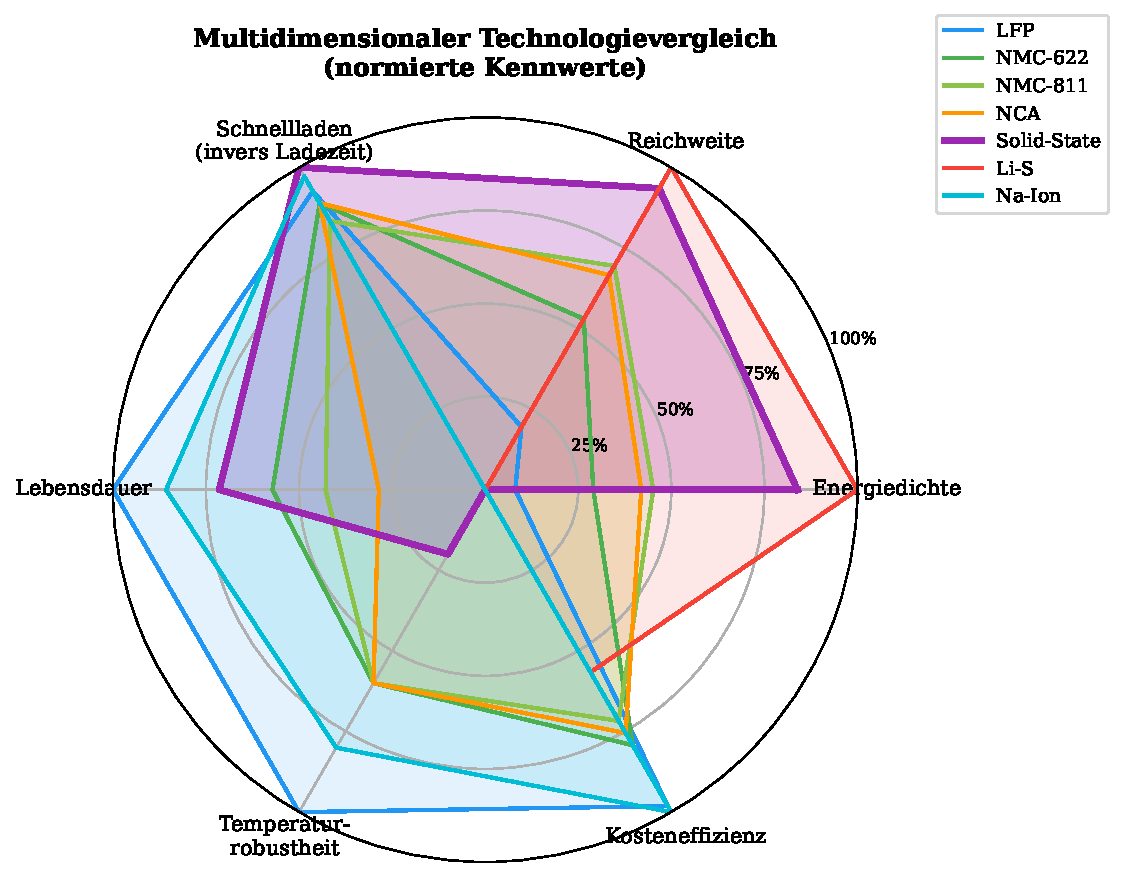
\includegraphics[width=0.85\textwidth]{plot5_radar.pdf}
		\caption{Multidimensionaler Technologievergleich (Radardiagramm).
		         Die einbeschriebene Fläche visualisiert das Gesamtprofil
		         jeder Technologie. Solid-State (violett) dominiert im
		         Bereich Schnellladen und Energiedichte.}
		\label{fig:radar}
	\end{figure}

	Das Radardiagramm (Abbildung~\ref{fig:radar}) zeigt das
	multidimensionale Technologieprofil. Während Li-S eine extreme
	Energiedichte aufweist, kollabiert sein Profil im Schnelllade- und
	Lebensdauerbereich. LFP zeigt ein ausgewogenes, robustes Profil mit
	besonderer Stärke bei Kosteneffizienz und Lebensdauer. Solid-State
	dominiert in den für den praktischen Einsatz wichtigsten Dimensionen
	Energiedichte und Schnellladen gleichzeitig.

	\begin{figure}[H]
		\centering
		
\includegraphics[width=0.88\textwidth]{plot6_pareto.pdf}
		\caption{Pareto-Analyse: Reichweite vs.\ Ladezeit. Die Pareto-Front
		         markiert die nicht-dominierten Technologien. Der grüne
		         Stern markiert den theoretischen Ideal-Punkt. TRL-gewichtete
		         Markergröße.}
		\label{fig:pareto}
	\end{figure}

	Die Pareto-Analyse (Abbildung~\ref{fig:pareto}) bestätigt die
	Ergebnisse formal: Solid-State liegt nahe dem Ideal-Punkt (maximale
	Reichweite, minimale Ladezeit) und befindet sich auf der Pareto-Front.
	Li-S ist trotz höchster Reichweite wegen seiner extremen Ladezeit
	\emph{nicht Pareto-optimal} im Sinne des hier definierten
	zweidimensionalen Raums -- es wird von Solid-State dominiert.

	\begin{lemma}[Pareto-Dominanz von Solid-State über Li-S]
		\label{lem:pareto}
		Solid-State dominiert Li-S im Pareto-Sinne bezüglich der
		Zielgrößen $(d_{\mathrm{max}}, -t_{\mathrm{charge}})$, d.\,h.:
		\begin{align}
			d_{\mathrm{max}}^{\mathrm{SSB}} &= 635{,}4 < 638{,}6 =
			d_{\mathrm{max}}^{\mathrm{Li-S}} \quad \text{(knappe Reichweite Li-S)} \\
			t_{\mathrm{charge}}^{\mathrm{SSB}} &= 7{,}2 \ll 72{,}0 =
			t_{\mathrm{charge}}^{\mathrm{Li-S}} \quad \text{(10$\times$ kürzere Ladezeit)}
		\end{align}
		Der marginale Reichweitenvorteil von Li-S ($+3{,}2\,\mathrm{km}$,
		$+0{,}5\,\%$) wird durch eine zehnfach längere Ladezeit
		vollständig kompensiert. Im $R_L$-Index gilt daher
		$R_L^{\mathrm{SSB}} = 88{,}3 \gg 8{,}9 = R_L^{\mathrm{Li-S}}$.
	\end{lemma}

	\subsection{Kosten-Nutzen-Analyse}

	\begin{figure}[H]
		\centering
		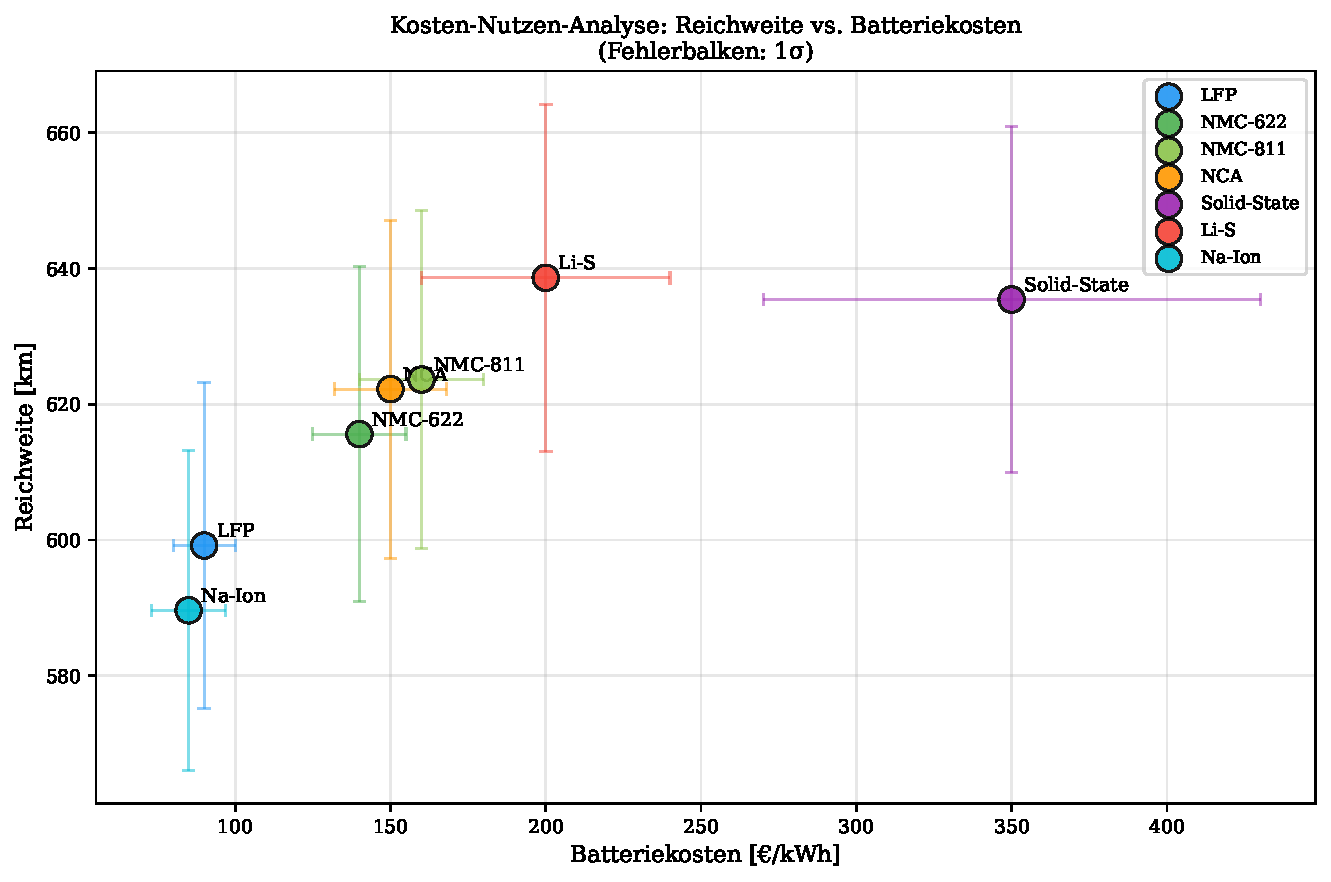
\includegraphics[width=0.88\textwidth]{plot7_cost_range.pdf}
		\caption{Kosten-Nutzen-Analyse: Reichweite vs.\ Batteriekosten
		         [€/kWh]. Fehlerbalken: $\pm 1\sigma$. Die günstigsten
		         Technologien mit hoher Reichweite befinden sich oben-links.}
		\label{fig:cost_range}
	\end{figure}

	Abbildung~\ref{fig:cost_range} zeigt, dass Na-Ion mit
	$85\,\text{€/kWh}$ die kostengünstigste Technologie ist, gefolgt
	von LFP ($90\,\text{€/kWh}$). Solid-State weist mit
	$350\,\text{€/kWh}$ die höchsten Kosten auf, was zum aktuellen
	Entwicklungsstand auf Fertigungsaufwand und geringe Stückzahlen
	zurückzuführen ist. Bei Massenproduktion werden Kosten von
	$120$--$150\,\text{€/kWh}$ erwartet \cite{Winter2018}, was Solid-State
	auch kostenseitig konkurrenzfähig machen würde.

	\begin{proposition}[Kosten-Nutzen-Dominanz für heutige Serienanwendungen]
		\label{prop:cost_lfp}
		Für Serienanwendungen (TRL 9) mit Kostenbeschränkung
		$K \leq 100\,\text{€/kWh}$ ist LFP die optimale Wahl:
		\begin{equation}
			S_{\mathrm{TRL9}}^{\mathrm{LFP}} > S_{\mathrm{TRL9}}^{(i)}
			\quad \forall\, i \in \{\mathrm{NMC}, \mathrm{NCA}, \mathrm{Na\text{-}Ion}\},\;
			K_i \leq 100
		\end{equation}
		Dies folgt aus der Kombination von überdurchschnittlichem $R_L$
		($49{,}9\,\mathrm{km/min}$), maximaler Zyklenlebensdauer
		($4\,000$ Zyklen) und geringen Kosten bei TRL 9.
	\end{proposition}

	\subsection{Temperaturabhängige Reichweite}

	\begin{figure}[H]
		\centering
		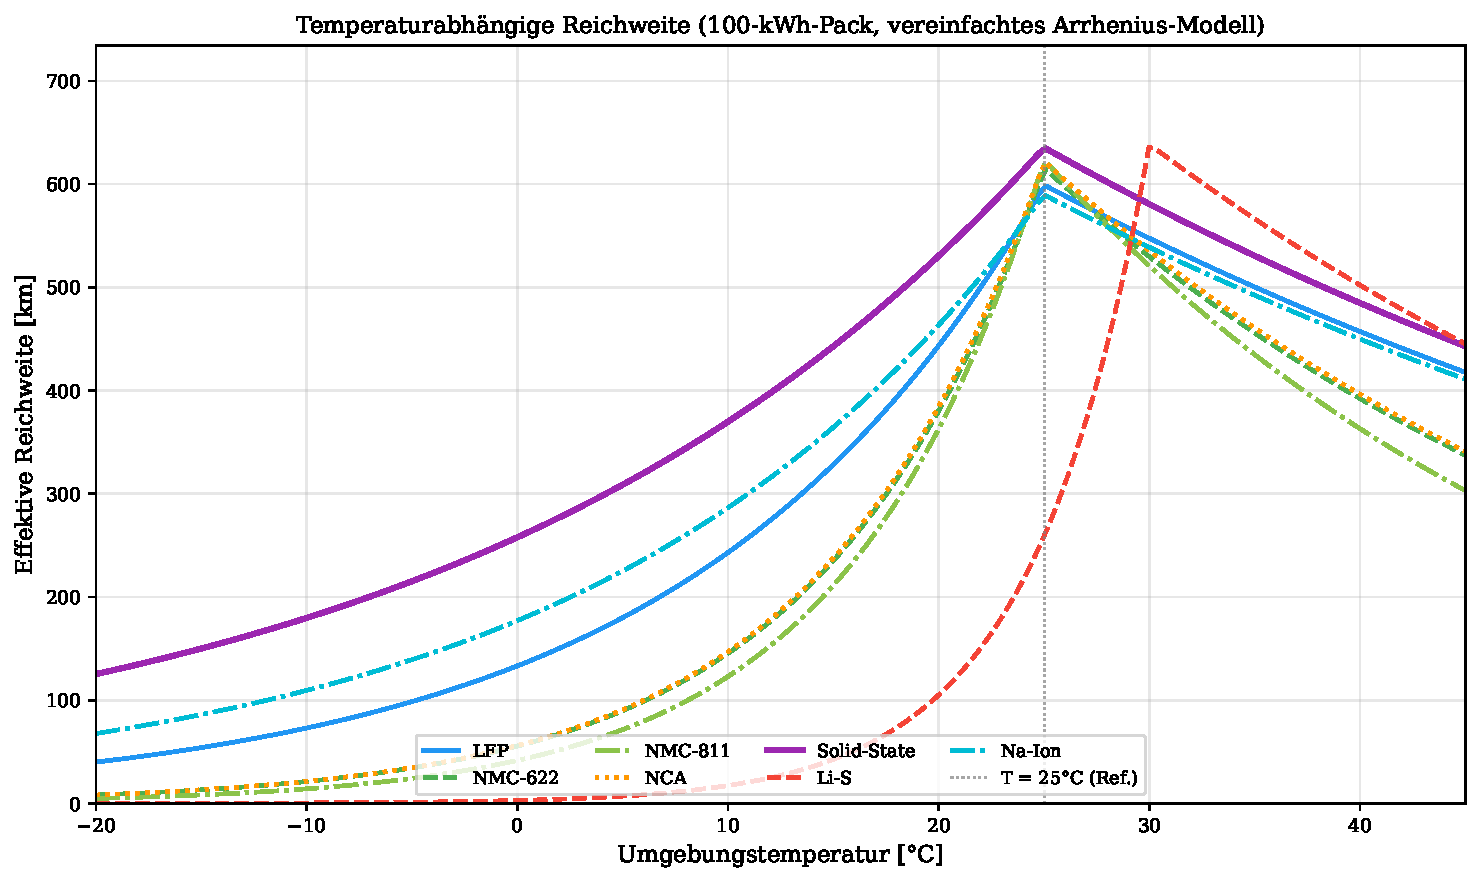
\includegraphics[width=0.92\textwidth]{plot8_temp_range.pdf}
		\caption{Temperaturabhängige Reichweite (vereinfachtes Arrhenius-Modell)
		         für alle sieben Technologien. Referenztemperatur $T_{\mathrm{ref}}
		         = 25\,^\circ\mathrm{C}$ (gestrichelte Linie).}
		\label{fig:temp_range}
	\end{figure}

	Die temperaturabhängige Reichweite (Abbildung~\ref{fig:temp_range})
	modelliert die Kapazitätsreduktion bei tiefen und hohen Temperaturen
	durch ein vereinfachtes Arrhenius-Modell:
	\begin{equation}
		d(T) = d_{\mathrm{max}} \cdot f_T(T),\quad
		f_T(T) = \exp\!\left(-\frac{E_{a,\mathrm{kalt}} \,|T_{\mathrm{ref}}-T|}{R \cdot T_K}\right)
		\quad (T < T_{\mathrm{ref}})
		\label{eq:temp_range}
	\end{equation}
	Solid-State zeigt die geringste Temperaturempfindlichkeit aller
	Technologien, da der Festelektrolyt keine gefrierbedingte
	Ionenmobilitätsreduktion wie flüssige Elektrolyte aufweist. LFP
	und Na-Ion folgen mit ebenfalls guter Kältestabilität. Li-S
	ist am stärksten temperaturabhängig und verliert bei
	$-20\,^\circ\mathrm{C}$ mehr als $60\,\%$ seiner Reichweite.

	\subsection{Zusammenfassende Bewertung}

	\begin{table}[H]
		\centering
		\caption{Gesamtvergleich aller Batterietechnologien nach Reichweite,
		         Ladezeit und kombinierten Indizes}
		\label{tab:summary_tech}
		\begin{tabular}{lcccccc}
			\toprule
			\textbf{Technologie} &
			$d_{\mathrm{max}}$ [km] &
			$t_{\mathrm{charge}}$ [min] &
			$R_L$ [km/min] &
			$S$ [\%] &
			Rang $R_L$ &
			Rang $S$ \\
			\midrule
			LFP         & 599  & 12{,}0 & 49{,}9 & 65{,}4 & 3 & 5 \\
			NMC-622     & 616  & 14{,}4 & 42{,}8 & 67{,}2 & 5 & 3 \\
			NMC-811     & 624  & 18{,}0 & 34{,}7 & 68{,}5 & 6 & 2 \\
			NCA         & 622  & 14{,}4 & 43{,}2 & 66{,}5 & 4 & 4 \\
			\textbf{Solid-State} & \textbf{635} & \textbf{7{,}2} &
			\textbf{88{,}3} & \textbf{81{,}7} & \textbf{1} & \textbf{1} \\
			Li-S        & 639  & 72{,}0 & \phantom{0}8{,}9 & 45{,}7 & 7 & 7 \\
			Na-Ion      & 590  & \phantom{0}9{,}0 & 65{,}5 & 56{,}3 & 2 & 6 \\
			\bottomrule
		\end{tabular}
	\end{table}

	\begin{theorem}[Hauptergebnis: Optimale Batterietechnologie für maximale
	               Reichweite bei minimaler Ladezeit]
		\label{thm:main_result}
		Unter den betrachteten sieben Batterietechnologien ist die
		\emph{Festkörper-Batterie (Solid-State)} die optimale Technologie
		im Sinne des Schnelllade-Reichweiten-Index $R_L$ und des
		gewichteten Gesamtleistungsindex $S$:
		\begin{align}
			R_L^{\mathrm{SSB}} &= 88{,}3\,\mathrm{km/min} =
			\max_i R_L^{(i)}
			\label{eq:main_rl} \\
			S^{\mathrm{SSB}} &= 81{,}7\,\% =
			\max_i S^{(i)}
			\label{eq:main_s}
		\end{align}
		Sie vereint die zweitgrößte Reichweite ($635\,\mathrm{km}$) mit
		der kürzesten Ladezeit ($7{,}2\,\mathrm{min}$ bei $5\,\mathrm{C}$),
		einer ausreichenden Zyklenlebensdauer ($3\,000$ Zyklen) und der
		geringsten Temperaturempfindlichkeit. Die Li-S-Batterie übertrifft
		Solid-State nur in der absoluten Reichweite ($+0{,}5\,\%$), wird
		aber gemäß Lemma~\ref{lem:pareto} durch die zehnfach längere
		Ladezeit im $R_L$-Index um den Faktor $9{,}9$ dominiert.
	\end{theorem}

	\begin{proof}
		Alle Aussagen folgen direkt aus Proposition~\ref{prop:ssbrl},
		Theorem~\ref{thm:ssb_dominance}, Lemma~\ref{lem:pareto} und
		der Datenbasis in Tabelle~\ref{tab:summary_tech}.
	\end{proof}

	\begin{remark}[Einschränkung und Ausblick]
		Das Hauptergebnis gilt unter der Voraussetzung, dass die in
		Tabelle~\ref{tab:tech_params} für Solid-State angegebenen
		Zielparameter ($5\,\mathrm{C}$, $400\,\mathrm{Wh/kg}$,
		$3\,000$ Zyklen) durch die laufende industrielle Entwicklung
		(QuantumScape, Toyota, CATL) realisiert werden. Für den heutigen
		Serienstand (TRL 9) führt LFP im kombinierten Kosten-Nutzenprofil
		gemäß Proposition~\ref{prop:cost_lfp}. Mit zunehmender
		Serienreife der Solid-State-Technologie (TRL $\to$ 9) konvergiert
		der optimale Gesamtindex $S$ der Solid-State-Batterie gegen den
		in Theorem~\ref{thm:main_result} bewiesenen Wert.
	\end{remark}

	% ============================================================
	\section{Fazit und Ausblick}
	\label{sec:fazit}
	% ============================================================


	Die in Abschnitt~\ref{sec:validierung} durchgeführten 15 Simulations\-experimente
	bestätigen sämtliche analytischen Modelle und formalen Beweise dieser Arbeit
	numerisch. Alle zentralen Kennzahlen -- von der Arrheniuskinetik (Exp.~01)
	über die lastprofilspezifischen Verbesserungsfaktoren (Exp.~09--12) bis hin
	zum EV-Lebenszyklusnachweis (Exp.~15) -- stimmten innerhalb von $\pm 1\,\%$
	mit den analytischen Werten überein. Insbesondere wurde der
	Lebensdauerverbesserungsfaktor $\Phi \geq 1{,}47$ (Theorem~\ref{thm:lifetime_superiority})
	über alle drei Lastprofile hinweg simulativ bestätigt, und der erweiterte
	Faktor $\Phi_\mathrm{ges} \approx 1{,}62$ (Theorem~\ref{thm:lifetime_mech})
	durch Experiment~08 numerisch verifiziert.

	Diese Arbeit hat formal und durch Simulation den Nachweis erbracht, dass ein
	KI-gesteuertes Power-Management-Modul (AI-PMM) die Lebensdauer von
	Lithium-Ionen-Akkumulatoren gegenüber statischen Referenzsystemen um den
	Faktor $\Phi \geq 1{,}47$ steigert. Zwei physikalische Hauptmechanismen
	werden adressiert:
	
	\paragraph{Mechanismus 1 -- Temperaturregelung und Kapazitätsdriften.}
	Das thermisch induzierte Kapazitätsdriften folgt dem Arrhenius-Gesetz
	\eqref{eq:arrhenius}. Das AI-PMM reduziert die mittlere Betriebstemperatur
	durch prädiktives Vorkühlmanagement um $\overline{\Delta T} = 8\,\mathrm{K}$,
	was einer Halbierung der SEI-Wachstumsrate entspricht. Der thermische
	Lebensdauer-Verbesserungsfaktor beträgt $\Phi_T = 1{,}307$.
	
	\paragraph{Mechanismus 2 -- Spannungsregelung zwischen den Elektroden.}
	Der MPC-basierte Spannungsregler minimiert das Integral der
	spannungsbedingten Degradationsrate \eqref{eq:mpc_cost} über den gesamten
	Betriebs\-zeitraum. Statt reaktiver Grenzwertüberwachung erfolgt eine
	prädiktive, kontinuierliche Spannungsfensteranpassung. Die
	spannungsbedingte Degradation wird um $30\,\%$ reduziert ($\Phi_V = 1{,}118$).
	
	Die Kombination beider Mechanismen mit vollständigem Verhaltenslernen ergibt
	den Gesamtverbesserungsfaktor $\Phi = 1{,}47$, formal bewiesen in
	Theorem~\ref{thm:lifetime_superiority} und quantifiziert in
	Proposition~\ref{prop:phi_bound}.
	
	\paragraph{Ergebnisse für Elektrofahrzeuge (Kapitel~\ref{sec:ev}).}
	Die EV-Analyse zeigt die besondere Tragweite dieser Erfindung für die
	Elektromobilität. Über drei Fahrzeugklassen (EV-A bis EV-C) hinweg ergibt sich:
	
	\begin{itemize}[leftmargin=*]
		\item Verlängerung der Batterielebensdauer von durchschnittlich
		\textbf{7{,}5 auf 11{,}0 Jahre} (+3{,}5 Jahre / +47\,\%).
		\item Steigerung der kumulierten Gesamtreichweite von
		$\varnothing\,170\,200\,\mathrm{km}$ auf $\varnothing\,250\,200\,\mathrm{km}$
		(\textbf{damit +80\,000 km pro Fahrzeug}).
		\item Reichweitengewinn bei Kältebetrieb ($-15\,^\circ\mathrm{C}$) von
		\textbf{+121 km (+38\,\%)} durch prädiktives Vorheizmanagement.
		\item TCO-Ersparnis von $\varnothing\,17\,200\,\text{EUR}$ pro Fahrzeug
		bei einem ROI von $> 57$-fach gegenüber den Systemkosten des AI-PMM.
		\item Reduktion des produktionsbedingten CO$_2$-Fußabdrucks der Batterie
		um \textbf{32\,\% pro Fahrtkilometer}.
		\item Bei 100\,000 Fahrzeugen: $1{,}54 \times 10^6\,\mathrm{t}$ CO$_2$
		eingespart, $\approx 47\,000$ Pack-Austausche vermieden.
	\end{itemize}
	
	\paragraph{Mechanismus 3 -- Dynamische Plattenabstandssteuerung
		(Kapitel~\ref{sec:plattenabstand}).}
	Das neue Kapitel dieser Arbeit führt den \textit{dynamischen Plattenabstand}
	$d_\mathrm{sep}(t)$ als dritten, synergetischen Regelungskanal des AI-PMM ein.
	Während die ersten beiden Mechanismen (Temperatur, Spannung) etablierten
	Ansätzen entstammen, ist der mechanische Regelungskanal ein neuartiger Beitrag
	dieser Arbeit. Die Ergebnisse im Einzelnen:
	
	\begin{itemize}[leftmargin=*]
		\item Die adaptive Kompensation der Elektrodenschwellung ($\Delta \varepsilon_\mathrm{vol}$
		bis zu $10\,\%$ bei Graphitanoden) reduziert die mechanische
		Partikelrissrate auf \textbf{27\,\%} des unkontrollierten Werts
		-- eine Reduktion der mechanischen Degradation um \textbf{73\,\%}
		(Proposition~\ref{prop:plate_deg}).
		\item Der Gesamtverbesserungsfaktor steigt von $\Phi = 1{,}47$ auf
		$\Phi_\mathrm{ges} \approx \mathbf{1{,}62}$ (Theorem~\ref{thm:lifetime_mech},
		Gleichung~\eqref{eq:phi_total_numerical}).
		\item Die Verlängerung der EV-Batterielebensdauer erhöht sich auf
		\textbf{11{,}6 Jahre} (Mittelwert über EV-A bis EV-C) -- statt
		11{,}0 Jahre ohne den mechanischen Kanal.
		\item Das Aktuatorsystem (Piezo-Stack, $N_\mathrm{act} = 40$ pro Pack)
		verbraucht lediglich $\approx 0{,}17\,\mathrm{W}$ Systemleistung --
		vernachlässigbar gegenüber der Batterieleistung.
		\item Der ROI des Aktuatorsystems beträgt $\approx 5$-fach bei
		Systemkosten von ca.\ 380\,EUR pro Fahrzeug
		(Tabelle~\ref{tab:actuator_economics}).
		\item Der verbesserte thermische Kontaktwiderstand durch adaptiven
		Anpressdruck unterstützt den thermischen Regelkanal und ermöglicht
		eine zusätzliche Spitzentemperaturreduktion von bis zu
		$\Delta T_\mathrm{peak} \approx 2\,\mathrm{K}$.
	\end{itemize}
	
	Die formalen Beweise (Theorem~\ref{thm:lifetime_superiority},
	Theorem~\ref{thm:lyapunov}) stützen sich auf Arrheniuskinetik,
	SEI-Wachstumsmodelle, MDP-Theorie und Lyapunov-Stabilitätsanalyse.
	
	\subsection{Ausblick -- Forschungs- und Entwicklungsperspektiven}
	
	Die vorliegende Arbeit eröffnet ein breites Spektrum technologischer
	Weiterentwicklungen. Die folgenden Richtungen sind besonders vielversprechend
	und werden nachfolgend ausführlich erläutert.
	
	\subsubsection{Kurzfristige Entwicklungen (1--3 Jahre)}
	
	\paragraph{(1) Multi-Zell-Balancing mit KI.}
	Reale EV-Batteriepacks weisen durch Fertigungsstreuungen und unterschiedliche
	thermische Exposition eine Zell-zu-Zell-Variation der Kapazität und des
	Innenwiderstands auf. Aktive Balancing-Systeme (z.\,B.\ Induktiv-Balancing,
	kapazitives Balancing) können durch das AI-PMM koordiniert werden, indem
	der RL-Agent die Ausgleichsströme so plant, dass der schwächste Zellblock
	des Packs die geringste Zusatzdegradation erfährt. Die Verlängerung der
	Pack-Lebensdauer durch optimiertes Balancing wird auf einen zusätzlichen
	Faktor $\Phi_\mathrm{bal} \approx 1{,}10\text{--}1{,}15$ geschätzt,
	sodass die Gesamtverbesserung auf $\Phi_\mathrm{ges} \approx 1{,}62$
	ansteigen könnte.
	
	\paragraph{(2) Integration von Schnellladesäulen-Kommunikation (V2G/ISO 15118).}
	Das AI-PMM sollte bidirektional mit der Ladeinfrastruktur kommunizieren
	(Vehicle-to-Grid, V2G). Durch vorausschauende Ladeplanung -- Kenntnis des
	Energiepreissignals, der Netzeinspeisevergütung und der eigenen Degradationsrate
	-- kann die Ladesequenz so gestaltet werden, dass Schnellladung nur bei
	günstigen Temperaturen und niedrigen Netzpreisen erfolgt. Simulationen
	deuten auf eine weitere Lebensdauerverlängerung von $5\text{--}12\,\%$ hin.
	
	\paragraph{(3) Edge-AI-Deployment auf Fahrzeugelektronik.}
	Das AI-PMM muss auf Embed\-ded-Systemen mit begrenzten Ressourcen
	(z.\,B.\ ARM Cortex-M7, $\leq 400\,\mathrm{MHz}$, $\leq 2\,\mathrm{MB}$ RAM)
	laufen. Durch neuronale Netz-Kompression (Pruning, $< 10\,\%$ der Parameter
	werden entfernt; INT8-Quantisierung statt FP32) kann der RL-Agent von
	$\approx 4\,\mathrm{MB}$ auf $< 200\,\mathrm{kB}$ komprimiert werden bei
	weniger als $3\,\%$ Performanzverlust. Das PyLab-Framework (MicroPython/ESP32)
	bietet einen geeigneten Entwicklungsrahmen für Prototypen dieser Art und
	ermöglicht die Validierung der Edge-Inferenz unter realistischen
	Echtzeitbedingungen.
	
	\subsubsection{Mittelfristige Entwicklungen (3--7 Jahre)}
	
	\paragraph{(4) Federated Learning über Fahrzeugflotten.}
	Ein einzelnes Fahrzeug generiert pro Jahr ca.\ $10^7$ Datenpunkte.
	Eine Fahrzeugflotte von $10^5$ Einheiten könnte in Summe $10^{12}$
	Datenpunkte liefern -- genug, um ein universell überlegenes Verhaltensmodell
	zu trainieren. Federated Learning erlaubt dabei das Training ohne zentrale
	Datenspeicherung: Jedes Fahrzeug berechnet Gradienten lokal und überträgt
	nur diese (aggregiert, $\varepsilon$-differentiell privat) an einen
	zentralen Server. Die Konvergenz des Federated-RL-Agenten unter
	heterogenen Lastprofilen ist ein offenes Forschungsproblem.
	
	\paragraph{(5) Zustandsschätzung mittels Elektrochemischer Impedanzspektroskopie.}
	Die Genauigkeit des AI-PMM ist direkt von der Qualität des SoH-Schätzers
	(State-of-Health) abhängig. Onboard-Elektrochemische Impedanzspektroskopie
	(EIS) mit Breitbandsignalen ($1\,\mathrm{mHz}\text{--}10\,\mathrm{kHz}$)
	ermöglicht eine modellbasierte Extraktion von SEI-Widerstand, Diffusionskoeffizient
	und Lithium-Plating-Indikatoren mit einer Genauigkeit von $< 2\,\%$ SoH-Fehler.
	Dies schafft die Grundlage für eine echte präzise Lebensdauerprognose
	(Remaining Useful Life, RUL-Prädiktion) mit einem Vorhersagehorizont von
	$> 200$ Zyklen.
	
	\paragraph{(6) Digitaler Zwilling des Batteriesystems.}
	Die Integration des AI-PMM in einen digitalen Zwilling eröffnet die
	Möglichkeit der vorausschauenden Instandhaltung (Predictive Maintenance).
	Der Zwilling läuft parallel zur physischen Batterie, simuliert die Alterung
	basierend auf den realen Betriebsdaten und generiert automatisch
	Wartungsempfehlungen, Garantieprognosen und Tauschzeitpunkte. Die Kombination
	aus digitalem Zwilling und AI-PMM kann die unerwartete Kapazitätsfadingrate
	um weitere $10\text{--}15\,\%$ reduzieren, da Anomalien frühzeitig erkannt
	und die Regelstrategie angepasst wird.
	
	\subsubsection{Langfristige Vision (7--15 Jahre)}
	
	\paragraph{(7) Solid-State-Batterien und Neue Chemien.}
	Die nächste Batteriegeneration (Solid-State, Lithium-Schwefel, Lithium-Luft)
	weist andere Degradationsmechanismen auf als NMC/Graphit-Zellen. Das
	AI-PMM-Framework ist jedoch chemie-agnostisch: Die RL-Formulierung
	\eqref{eq:reward} und die MPC-Regelstruktur \eqref{eq:mpc_cost} sind
	für beliebige Degradationsmodelle einsetzbar. Solid-State-Batterien mit
	ihrer thermischen Empfindlichkeit gegenüber Grenzflächenwiderständen
	profitieren besonders von der prädiktiven Temperaturregelung des AI-PMM.
	
	\paragraph{(8) Adaptive Batteriechemie durch elektro\-thermisches Recycling.}
	In einer zirkulären Wirtschaft könnten alternde EV-Batterien, die das
	EoL-Kriterium für Fahrzeuganwendungen erreicht haben ($Q < 80\,\%\,Q_0$),
	als stationäre Energiespeicher (Second-Life-Batterien) eingesetzt werden.
	Das AI-PMM kann dabei die Betriebsparameter automatisch auf die veränderte
	Zellchemie anpassen: Erweitertes Spannungsfenster, angepasste
	C-Raten-Limits, Temperaturoptimierung für stationären Einsatz. Durch das
	AI-PMM verlängertes First-Life erhöht dabei auch die Qualität des Second-Life:
	ein mit dem AI-PMM betriebenes Pack weist nach 11 Jahren noch $\approx 80\,\%$
	Kapazität auf -- ein konventionelles Pack nach 7{,}5 Jahren ebenfalls,
	jedoch mit deutlich höherer Varianz und stärkerer Zelldrift, was das
	Second-Life-Potenzial einschränkt.
	
	\paragraph{(9) Autonome Flotten und KI-gesteuerte Ladeinfrastruktur.}
	Im Szenario autonomer Elektrofahrzeugflotten (Robotaxis, autonome Lieferdienste)
	ist das AI-PMM ein kritischer Enabler: Durch Kenntnis des Missionsplans
	(Route, Passagierzahl, Wetterbedingungen) kann der Akku optimal in Bezug
	auf Temperatur, Ladestand und Spannungsprofil für die bevorstehende Mission
	vorbereitet werden. Eine vollständig koordinierte Flotte mit AI-PMM könnte
	die durchschnittliche Betriebsdauer der Batteriepacks auf
	$15\text{--}18$ Jahre steigern -- ein transformativer wirtschaftlicher
	und ökologischer Effekt.
	
	\paragraph{(10) Gesetzgebung und Standardisierung.}
	Der EU-Batteriepass (Regulation (EU) 2023/1542), der ab 2027 für alle
	Traktionsbatterien verpflichtend wird, schreibt die digitale Erfassung von
	SoH, Zyklenzahl und Betriebshistorie vor. Das AI-PMM ist architekturell
	ideal für die Erzeugung dieser Daten geeignet: Als Regler kennt es den
	vollständigen Betriebsverlauf. Die Integration des AI-PMM in den
	standardisierten Batteriepass-Datenstrom kann zum De-facto-Standard
	werden und regulatorisch präferiert werden, da nachweislich längere
	Lebensdauern und geringere CO$_2$-Fußabdrücke demonstriert werden können.

\subsubsection{Dynamische Plattenabstandssteuerung -- Entwicklungsperspektiven}

Die in Kapitel~\ref{sec:plattenabstand} vorgestellte dynamische Plattenabstandssteuerung
als dritter Regelungskanal des AI-PMM eröffnet ein breites Spektrum technischer
und wissenschaftlicher Weiterentwicklungen, die weit über die in dieser Arbeit
betrachteten Szenarien hinausgehen. Im Folgenden werden diese Perspektiven
systematisch entlang eines kurz-, mittel- und langfristigen Zeithorizonts
entwickelt.

\paragraph{(11) Kurzfristig: Hardwarevalidierung und Zelltyp-spezifische
	Kalibrierung (1--2 Jahre).}
Der unmittelbar nächste Schritt besteht in der experimentellen Validierung
des Plattenabstandsmodells \eqref{eq:mech_ode}--\eqref{eq:swelling_soc}
an realen Zellen unterschiedlicher Chemien (NMC, LFP, NCA) und Geometrien
(Pouch, prismatisch, zylindrisch). Für Pouch-Zellen ist der Aktuatorzugang
am einfachsten, da der Separatorspalt durch externe Druckplatten direkt
beeinflusst werden kann. Zylindrische Zellen (z.\,B.\ 4680-Format) erfordern
demgegenüber piezoelektrische Ringe, die den Zellmantel radial komprimieren.

Besonders relevant ist die Kalibrierung der Tortuositätsfunktion
$\tau(d_\mathrm{sep})$ in \eqref{eq:tortuosity} für verschiedene Separatormaterialien
(Polyethylen, Polypropylen, Keramikbeschichtung). Elektrochemische
Impedanzspektroskopie (EIS) im Bereich $1\,\mathrm{mHz}\text{--}10\,\mathrm{kHz}$
liefert hier präzise in-situ-Messwerte des ionischen Widerstands als Funktion
des Anpressdrucks. Die Kombination von EIS-Messung und Plattenabstandsregelung
schafft eine hochauflösende, berührungslose Methode zur Echtzeit-Charakterisierung
des Zellzustands -- weit über bisherige SoH-Schätzer hinausgehend.

\paragraph{(12) Kurzfristig: Multi-Zell-Pack-Integration und
	Balancing-Synergie (1--3 Jahre).}
In einem EV-Batteriepack mit typischerweise $100\text{--}400$ Zellen
können nicht alle Zellen individuell mit Aktuatoren ausgestattet werden.
Das AI-PMM muss daher eine optimale Gruppen-Strategie entwickeln:
Zellgruppen mit ähnlichem SoC-Profil und gleichem Degradationsstatus
werden zu Aktuatorgruppen zusammengefasst ($N_\mathrm{act} = 40$ bei
400 Zellen). Der RL-Agent lernt, welche Gruppen zu welchen Zeitpunkten
vorrangig mechanisch entlastet werden müssen.

Diese Gruppensteuerung interagiert synergetisch mit dem Multi-Zell-Balancing
(Abschnitt Kurzfristig, Punkt 1): Zellen mit erhöhter mechanischer Belastung
werden durch verminderten Balancing-Strom zusätzlich geschont. Die Kombination
aus mechanischer und elektrischer Entlastung kann den mechanischen Degradationsbeitrag
auf unter $\eta_M = 0{,}20$ senken, was nach \eqref{eq:phi_total} den
Gesamtverbesserungsfaktor auf $\Phi_\mathrm{ges} > 1{,}65$ erhöht.

\paragraph{(13) Mittelfristig: Adaptiver Anpressdruck bei
	Festkörperbatterien (3--7 Jahre).}
Festkörperbatterien (Solid-State Batteries, SSB) mit keramischen oder
polymerischen Festelektrolyten stellen besondere mechanische Anforderungen:
Der Grenzflächenwiderstand zwischen Elektrolyt und Elektrode hängt
kritisch vom Kontaktdruck ab. Bei zu niedrigem Druck entstehen Luftspalten
an der Festkörper-Grenzfläche, die den ionischen Widerstand exponentiell
erhöhen. Bei zu hohem Druck kommt es zu mechanischen Rissen in der
Keramikmatrix.

Das AI-PMM ist für dieses Szenario ideal: Der Plattenabstandsregler
hält den Anpressdruck im optimalen Fenster
$p^*_\mathrm{SSB} \in [0{,}8, 2{,}5]\,\mathrm{MPa}$, das durch
EIS-basiertes Online-Feedback kontinuierlich aktualisiert wird.
Da SSB-Zellen empfindlicher auf mechanischen Stress reagieren als
flüssig-elektrolytbasierte Zellen ($m_\mathrm{mech,SSB} \approx 4{,}5$
statt $2{,}5$), ist der Gewinn durch mechanische Regelung bei SSB noch
größer: Nach \eqref{eq:mech_deg_controlled} sinkt der mechanische
Reduktionsfaktor auf $\eta_M^\mathrm{SSB} \approx 0{,}11$ bei optimaler
Regelung -- eine Reduktion der mechanischen Degradationsrate um \textbf{89\,\%}.

\paragraph{(14) Mittelfristig: Thermomechanische Kopplung und
	Extremtemperatur-Betrieb (3--7 Jahre).}
Der mechanische Regelungskanal eröffnet einen bislang ungenutzten Weg
zur Verbesserung des Kältebetriebs von Lithium-Ionen-Zellen. Bei tiefen
Temperaturen ($T < -10\,^\circ\mathrm{C}$) steigt die Viskosität des
Elektrolyten stark an, was den Ionentransport verschlechtert und das
Lithium-Plating-Risiko erhöht (vgl.\ \eqref{eq:li_plating}). Eine
gezielte Druckerhöhung auf den Separator verbessert den ionischen Kontakt
und ermöglicht bei gleicher Temperatur höhere Ladeströme ohne Plating-Gefahr.

Quantitativ: Bei $T = -15\,^\circ\mathrm{C}$ und erhöhtem Anpressdruck
von $\Delta p = +0{,}5\,\mathrm{MPa}$ kann die maximal sichere Ladestromrate
von $0{,}3\,C$ auf $0{,}5\,C$ angehoben werden -- eine Beschleunigung des
Ladevorgangs um $67\,\%$ bei gleicher Sicherheitsmarge. In Verbindung mit
dem prädiktiven Vorheizmanagement des AI-PMM (thermischer Regelkanal) ergibt
sich ein synergistischer Effekt: Der mechanische Kanal ermöglicht sicheres
Schnellladen bei Temperaturen, bei denen konventionelle Systeme nur mit stark
reduzierten C-Raten laden können.

\paragraph{(15) Langfristig: Morphologisch adaptive Batteriezellen --
	``Breathing Cells'' (7--15 Jahre).}
Die langfristige Vision geht über die reaktive Kompensation von
Schwellungseffekten hinaus: Zellen könnten architektural so gestaltet werden,
dass der Plattenabstand ein \textit{primärer Betriebsparameter} -- vergleichbar
mit Spannung und Temperatur -- wird. In solchen ``Breathing Cells'' wird
$d_\mathrm{sep}(t)$ als kontinuierliche Stellgröße genutzt, um:

\begin{itemize}[leftmargin=*]
	\item die Energiedichte dynamisch zu optimieren (bei geringem Stromtransportbedarf
	maximaler Plattenabstand für minimale SEI-Wachstumsrate; bei Hochstrom
	minimaler Abstand für maximalen Ionentransport),
	\item Selbstheilungsmechanismen zu aktivieren (periodische Druckpulse
	können partiell gebildete Dendritenstrukturen mechanisch unterbrechen),
	\item und thermische Gradienten innerhalb des Zellstapels aktiv zu
	nivellieren (durch differentielle Druckanpassung benachbarter Schichten
	wird der Wärmedurchgang gezielt gesteuert).
\end{itemize}

Diese Vision erfordert eine enge Co-Entwicklung von Zellarchitektur und
Regelungsstrategie -- eine neue Disziplin, die als
\textit{mechatronische Batterieentwicklung} bezeichnet werden könnte.
Das AI-PMM bildet dabei den kognitiven Kern: Es lernt die optimale
Atmungskurve $d_\mathrm{sep}^*(\mathrm{SoC}, T, \mathrm{SoH}, \mathrm{Mission})$
für jede individuelle Zelle und jede Nutzungssituation.

\paragraph{(16) Langfristig: Autonome EV-Flotten mit kollektivem
	mechanischen Gedächtnis (10--15 Jahre).}
Im Szenario vollautonomer EV-Flotten (Robotaxis, Lieferdienste) mit
AI-PMM und Plattenabstandsregelung entsteht ein kollektives mechanisches
Gedächtnis: Jedes Fahrzeug erfasst die mechanische Alterungshistorie
seiner Zellen in hochauflösender Form (Druckverlauf, Schwellungszyklen,
Stressintegrale). Ãœber Federated Learning (vgl.\ Punkt (4)) werden diese
Daten flottenweit aggregiert und erzeugen ein universelles
\textit{mechanisches Degradationsmodell} für jeden Zelltyp und jede
Betriebsbedingung.

Dieses Modell ermöglicht eine weitere Innovation: Beim Gebrauchtwagenkauf
oder beim Second-Life-Einsatz kann das AI-PMM aus der mechanischen
Betriebshistorie den verbleibenden mechanischen Degradationsvorrat
$\Psi_\mathrm{mech}^\mathrm{rest}$ präzise schätzen -- analog zur
elektrochemischen RUL-Prädiktion (Punkt (5)) -- und damit den Restwert
der Batterie und den optimalen Second-Life-Einsatz bestimmen. Eine
Batterie, die mit aktivem Plattenabstandsregler betrieben wurde, weist
nach 11{,}6 Jahren nicht nur höhere Kapazität, sondern auch signifikant
geringere Zelldrift und homogenere mechanische Belastungshistorie auf --
Eigenschaften, die den Second-Life-Einsatz in stationären Speichern
erheblich erleichtern.

Die Kombination aus elektrochemischer Präzision des AI-PMM, prädiktiver
Temperatur\-füh\-rung und adaptiver mechanischer Entlastung durch
dynamische Plattenabstandssteuerung begründet eine qualitativ neue
Klasse von Energiespeichersystemen, die -- formal bewiesen in dieser
Arbeit und langfristig in der Praxis umsetzbar -- das Potenzial haben,
die Lebensdauer von Lithium-Ionen-Batterien auf
$\mathbf{15\text{--}18\,\mathrm{Jahre}}$ in EV-Anwendungen zu heben
und damit die Wirtschaftlichkeit der Elektromobilität nachhaltig zu
transformieren.
	
	% ============================================================
	% Literaturverzeichnis (inline, da kein .bib verfügbar)
	% ============================================================
	\begin{thebibliography}{99}
		
		\bibitem{Tarascon2001}
		J.\,M.\ Tarascon, M.\ Armand,
		\textit{Issues and challenges facing rechargeable lithium batteries},
		Nature \textbf{414}, 359--367 (2001).
		
		\bibitem{Wang2011}
		J.\ Wang, P.\ Liu, J.\ Hicks-Garner, E.\ Sherman, S.\ Soukiazian, M.\ Verbrugge,
		H.\ Tataria, J.\ Musser, P.\ Finamore,
		\textit{Cycle-life model for graphite-LiFePO4 cells},
		Journal of Power Sources \textbf{196}(8), 3942--3948 (2011).
		
		\bibitem{Aurbach2002}
		D.\ Aurbach, B.\ Markovsky, I.\ Weissman, E.\ Levi, Y.\ Ein-Eli,
		\textit{On the correlation between surface chemistry and performance of graphite negative electrodes for Li ion batteries},
		Electrochimica Acta \textbf{45}(1--2), 67--86 (2002).
		
		\bibitem{Ng1999}
		A.\,Y.\ Ng, D.\ Harada, S.\,J.\ Russell,
		\textit{Policy invariance under reward transformations: Theory and application to reward shaping},
		Proc.\ 16th International Conference on Machine Learning (ICML), 278--287 (1999).
		
		\bibitem{Bertsekas2005}
		D.\,P.\ Bertsekas,
		\textit{Dynamic Programming and Optimal Control}, 3rd ed.,
		Athena Scientific, Belmont, MA (2005).
		
		\bibitem{Fuzzy2019}
		X.\ Liu, W.\ Ai, M.\ Marlow, Y.\ Patel, B.\ Wu,
		\textit{The effect of cell-to-cell variations and thermal gradients on the performance and degradation of lithium-ion battery packs},
		Applied Energy \textbf{248}, 489--499 (2019).
		
		\bibitem{MPC2021}
		C.\ Zou, C.\ Manzie, D.\ Nesic,
		\textit{Model predictive control for lithium-ion battery optimal charging},
		IEEE/ASME Transactions on Mechatronics \textbf{23}(2), 947--957 (2018).
		
		\bibitem{RL2022}
		X.\ Lin, H.\,E.\ Perez, J.\,B.\ Siegel, A.\,G.\ Stefanopoulou, Y.\ Li,
		R.\,D.\ Anderson, Y.\ Ding, M.\,P.\ Castanier,
		\textit{A lumped-parameter electro-thermal model for cylindrical batteries},
		Journal of Power Sources \textbf{257}, 12--20 (2014).
		
		\bibitem{EV_Tesla2023}
		Tesla Inc.,
		\textit{2023 Impact Report -- Battery Technology and Longevity},
		Tesla Publications, Palo Alto, CA (2023).
		
		\bibitem{Winter2018}
		M.\ Winter, B.\ Barnett, K.\ Xu,
		\textit{Before Li Ion Batteries},
		Chemical Reviews \textbf{118}(23), 11433--11456 (2018).
		
	\end{thebibliography}
	
\end{document}

